\documentclass[a4paper,landscape,10pt]{article}
\usepackage[margin=10mm]{geometry}
\usepackage[T1]{fontenc}
\usepackage{lmodern}
\usepackage{helvet}
\renewcommand{\familydefault}{\sfdefault}
\usepackage{tikz}
\usetikzlibrary{arrows.meta}
\usepackage{xcolor}
\usepackage{booktabs}
\setlength{\parindent}{0pt}
\definecolor{ft0}{HTML}{CFE4F2}
\definecolor{ft1}{HTML}{FBE2B4}
\definecolor{ft2}{HTML}{D4E9CC}
\definecolor{ft3}{HTML}{E5D3EA}
\definecolor{ft4}{HTML}{F5CACA}
\pagestyle{empty}
\begin{document}

{\LARGE\bfseries Bilderwand -- layout candidates}\\[4pt]
{\small Target 180x120 cm $\pm$ 10.0 cm, nominal gap free in
[1.5, 6.0] cm, orientation fixed, sizes are measured outer dimensions.
Max.\ gap deviation = largest difference between an actual gap and the layout's nominal gap;
notches = parts of the outer border not covered by a frame or a regular gap. Ranked by a combined
score (gap uniformity first, border sharpness second, then number of frames).}\\[10pt]
\begin{minipage}[t]{0.6\textwidth}\vspace{0pt}
\begin{tabular}{@{}r l r r r r l c r@{}}
\toprule
\# & size (cm) & gap & frames & max dev & mean dev & notches & corners & entropy \\
\midrule
1 & 182.0 $\times$ 129.0 & 4 & 24 & 1.8 & 0.56 & none & 4/4 & 0.65 \\
2 & 184.0 $\times$ 115.0 & 2 & 20 & 2.0 & 0.65 & 4 cm & 4/4 & 0.75 \\
3 & 179.5 $\times$ 120.5 & 1.5 & 26 & 2.5 & 0.58 & 10 cm & 4/4 & 0.67 \\
4 & 172.5 $\times$ 125.5 & 2.5 & 25 & 3.5 & 0.70 & none & 4/4 & 0.75 \\
5 & 174.5 $\times$ 130.5 & 1.5 & 25 & 2.5 & 0.95 & 6 cm & 4/4 & 0.78 \\
6 & 172.5 $\times$ 125.5 & 2.5 & 25 & 3.8 & 0.69 & none & 4/4 & 0.78 \\
7 & 179.5 $\times$ 111.5 & 1.5 & 25 & 4.0 & 0.51 & none & 4/4 & 0.79 \\
8 & 181.5 $\times$ 129.5 & 3.5 & 24 & 3.0 & 0.64 & 6 cm & 4/4 & 0.77 \\
9 & 176.5 $\times$ 113.5 & 1.5 & 23 & 3.5 & 0.70 & none & 4/4 & 0.79 \\
10 & 182.5 $\times$ 129.5 & 3.5 & 23 & 4.0 & 0.86 & none & 4/4 & 0.82 \\
11 & 184.5 $\times$ 113.5 & 1.5 & 23 & 3.5 & 0.86 & 4 cm & 4/4 & 0.78 \\
12 & 177.5 $\times$ 118.5 & 2.5 & 22 & 3.0 & 0.83 & 4 cm & 4/4 & 0.72 \\
13 & 173.5 $\times$ 116.5 & 3 & 21 & 3.0 & 0.63 & 6 cm & 4/4 & 0.79 \\
14 & 176.0 $\times$ 125.0 & 2 & 20 & 3.0 & 0.91 & 4 cm & 4/4 & 0.77 \\
15 & 179.5 $\times$ 120.5 & 1.5 & 26 & 3.0 & 0.61 & 8 cm & 4/4 & 0.77 \\
16 & 179.5 $\times$ 120.5 & 1.5 & 26 & 2.5 & 0.60 & 13 cm & 4/4 & 0.77 \\
\bottomrule
\end{tabular}
\end{minipage}\hfill
\begin{minipage}[t]{0.36\textwidth}\vspace{0pt}
{\bfseries Inventory}\\[4pt]
\begin{tabular}{@{}c l l r@{}}
\toprule
 & outer w $\times$ h (cm) &  & have \\
\midrule
\tikz[baseline=-0.6ex]\fill[ft0,draw=black!60] (0,0) rectangle (1.2ex,1.2ex); & 20.5$\times$15.5 & L & 9 \\
\tikz[baseline=-0.6ex]\fill[ft0,draw=black!60] (0,0) rectangle (1.2ex,1.2ex); & 15.5$\times$20.5 & P & 2 \\
\tikz[baseline=-0.6ex]\fill[ft3,draw=black!60] (0,0) rectangle (1.2ex,1.2ex); & 32.5$\times$42.5 & P & 2 \\
\tikz[baseline=-0.6ex]\fill[ft3,draw=black!60] (0,0) rectangle (1.2ex,1.2ex); & 42.5$\times$32.5 & L & 1 \\
\tikz[baseline=-0.6ex]\fill[ft1,draw=black!60] (0,0) rectangle (1.2ex,1.2ex); & 32.5$\times$23.5 & L & 5 \\
\tikz[baseline=-0.6ex]\fill[ft1,draw=black!60] (0,0) rectangle (1.2ex,1.2ex); & 23.5$\times$32.5 & P & 1 \\
\tikz[baseline=-0.6ex]\fill[ft2,draw=black!60] (0,0) rectangle (1.2ex,1.2ex); & 25.5$\times$25.5 &  & 5 \\
\tikz[baseline=-0.6ex]\fill[ft4,draw=black!60] (0,0) rectangle (1.2ex,1.2ex); & 42.5$\times$52.5 & P & 1 \\
\tikz[baseline=-0.6ex]\fill[ft4,draw=black!60] (0,0) rectangle (1.2ex,1.2ex); & 52.5$\times$42.5 & L & 2 \\
\bottomrule
\end{tabular}
\\[8pt]
{\scriptsize Search parameters: target = 180x120, tol = 10.0, gap\_min = 1.5, gap\_max = 6.0, gap\_mode = free, delta = 0.5, slack\_rule = even, cost\_shape = huber, min\_frames = 10, frame\_bonus = 1.5, runs = 256, iters = 20 min, seed = 0, large\_area = 2000.0, large\_count = 2-3, large\_apart = True, large\_min\_dist = 70.0, entropy = 40.0}
\end{minipage}
\clearpage

\begin{minipage}[t]{0.74\textwidth}\vspace{0pt}
{\LARGE\bfseries Layout 1}\hspace{1.5em}{\large 182.0 $\times$ 129.0 cm \quad gap 4 cm \quad 24 frames}\\[8pt]
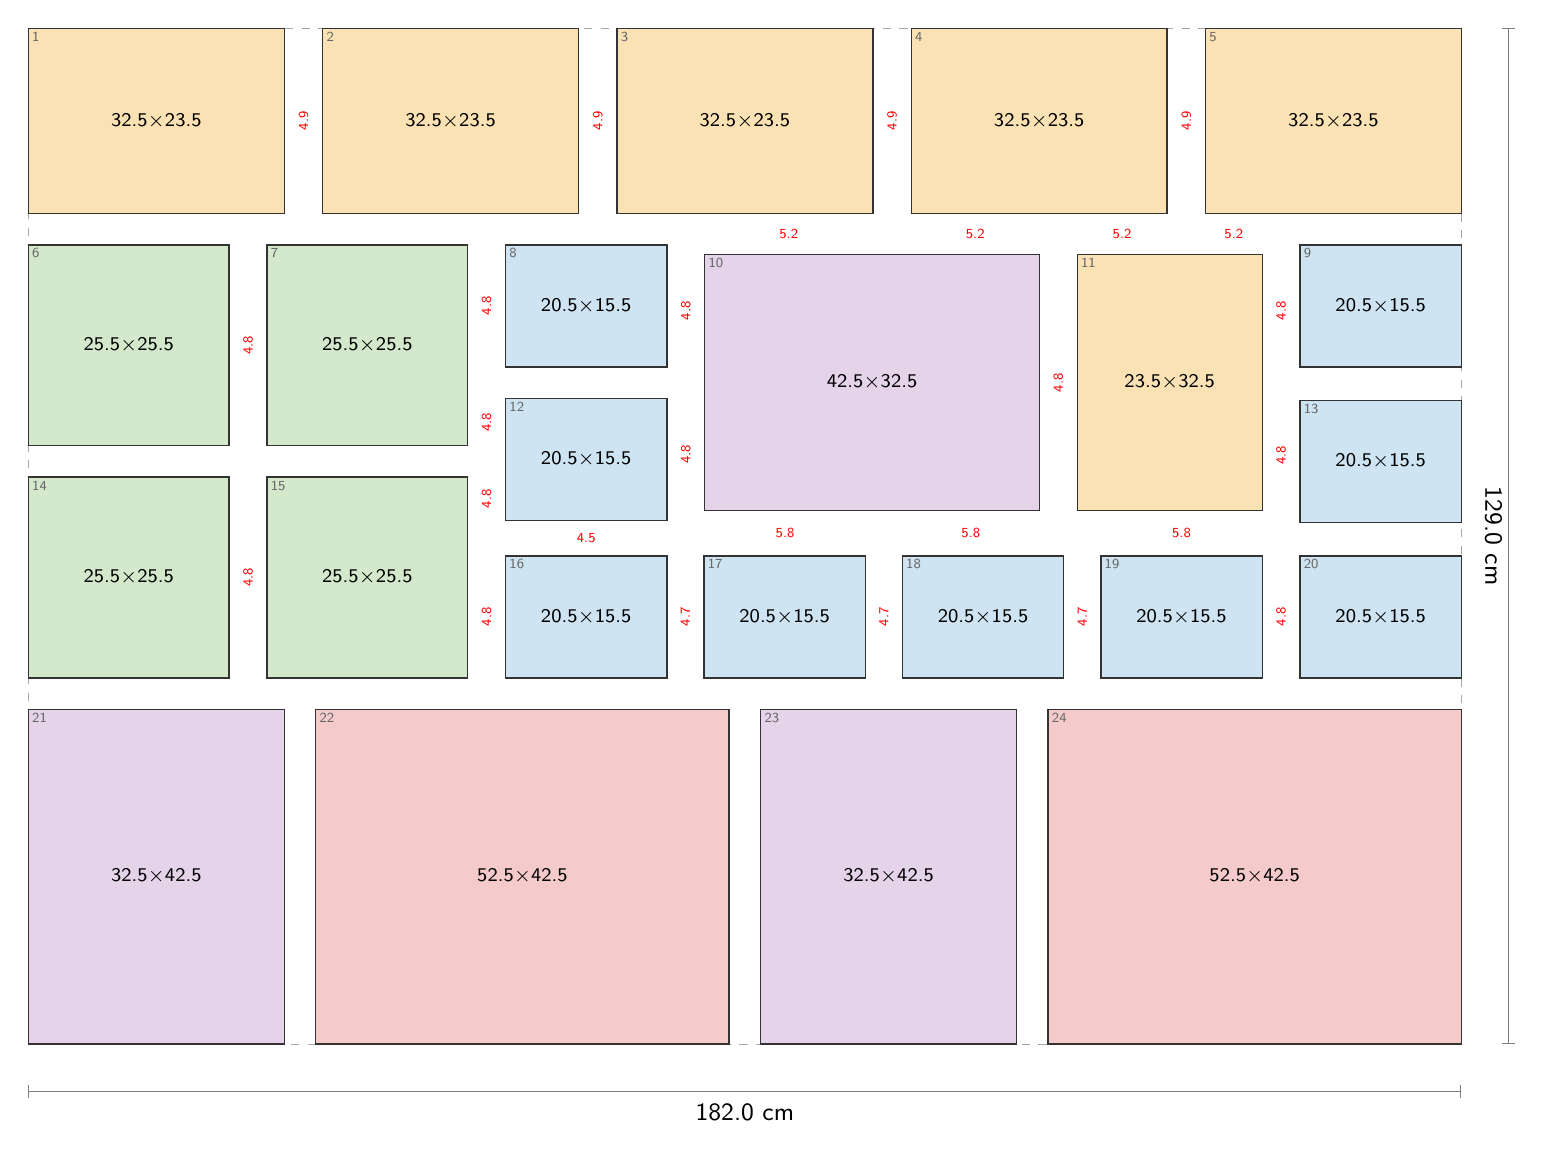
\begin{tikzpicture}[x=1mm, y=-1mm]
\draw[gray!70, dashed, line width=0.4pt] (0,0) rectangle (182.00,129.00);
\filldraw[fill=ft1, draw=black!80, line width=0.5pt] (0.00,0.00) rectangle (32.50,23.50);
\node[align=center, inner sep=0pt] at (16.25,11.75) {\scriptsize 32.5$\times$23.5};
\node[anchor=north west, inner sep=1.2pt, font=\tiny, text=black!60] at (0.00,0.00) {1};
\filldraw[fill=ft1, draw=black!80, line width=0.5pt] (37.38,0.00) rectangle (69.88,23.50);
\node[align=center, inner sep=0pt] at (53.62,11.75) {\scriptsize 32.5$\times$23.5};
\node[anchor=north west, inner sep=1.2pt, font=\tiny, text=black!60] at (37.38,0.00) {2};
\filldraw[fill=ft1, draw=black!80, line width=0.5pt] (74.75,0.00) rectangle (107.25,23.50);
\node[align=center, inner sep=0pt] at (91.00,11.75) {\scriptsize 32.5$\times$23.5};
\node[anchor=north west, inner sep=1.2pt, font=\tiny, text=black!60] at (74.75,0.00) {3};
\filldraw[fill=ft1, draw=black!80, line width=0.5pt] (112.12,0.00) rectangle (144.62,23.50);
\node[align=center, inner sep=0pt] at (128.38,11.75) {\scriptsize 32.5$\times$23.5};
\node[anchor=north west, inner sep=1.2pt, font=\tiny, text=black!60] at (112.12,0.00) {4};
\filldraw[fill=ft1, draw=black!80, line width=0.5pt] (149.50,0.00) rectangle (182.00,23.50);
\node[align=center, inner sep=0pt] at (165.75,11.75) {\scriptsize 32.5$\times$23.5};
\node[anchor=north west, inner sep=1.2pt, font=\tiny, text=black!60] at (149.50,0.00) {5};
\filldraw[fill=ft2, draw=black!80, line width=0.5pt] (0.00,27.50) rectangle (25.50,53.00);
\node[align=center, inner sep=0pt] at (12.75,40.25) {\scriptsize 25.5$\times$25.5};
\node[anchor=north west, inner sep=1.2pt, font=\tiny, text=black!60] at (0.00,27.50) {6};
\filldraw[fill=ft2, draw=black!80, line width=0.5pt] (30.30,27.50) rectangle (55.80,53.00);
\node[align=center, inner sep=0pt] at (43.05,40.25) {\scriptsize 25.5$\times$25.5};
\node[anchor=north west, inner sep=1.2pt, font=\tiny, text=black!60] at (30.30,27.50) {7};
\filldraw[fill=ft0, draw=black!80, line width=0.5pt] (60.60,27.50) rectangle (81.10,43.00);
\node[align=center, inner sep=0pt] at (70.85,35.25) {\scriptsize 20.5$\times$15.5};
\node[anchor=north west, inner sep=1.2pt, font=\tiny, text=black!60] at (60.60,27.50) {8};
\filldraw[fill=ft0, draw=black!80, line width=0.5pt] (161.50,27.50) rectangle (182.00,43.00);
\node[align=center, inner sep=0pt] at (171.75,35.25) {\scriptsize 20.5$\times$15.5};
\node[anchor=north west, inner sep=1.2pt, font=\tiny, text=black!60] at (161.50,27.50) {9};
\filldraw[fill=ft3, draw=black!80, line width=0.5pt] (85.90,28.75) rectangle (128.40,61.25);
\node[align=center, inner sep=0pt] at (107.15,45.00) {\scriptsize 42.5$\times$32.5};
\node[anchor=north west, inner sep=1.2pt, font=\tiny, text=black!60] at (85.90,28.75) {10};
\filldraw[fill=ft1, draw=black!80, line width=0.5pt] (133.20,28.75) rectangle (156.70,61.25);
\node[align=center, inner sep=0pt] at (144.95,45.00) {\scriptsize 23.5$\times$32.5};
\node[anchor=north west, inner sep=1.2pt, font=\tiny, text=black!60] at (133.20,28.75) {11};
\filldraw[fill=ft0, draw=black!80, line width=0.5pt] (60.60,47.00) rectangle (81.10,62.50);
\node[align=center, inner sep=0pt] at (70.85,54.75) {\scriptsize 20.5$\times$15.5};
\node[anchor=north west, inner sep=1.2pt, font=\tiny, text=black!60] at (60.60,47.00) {12};
\filldraw[fill=ft0, draw=black!80, line width=0.5pt] (161.50,47.25) rectangle (182.00,62.75);
\node[align=center, inner sep=0pt] at (171.75,55.00) {\scriptsize 20.5$\times$15.5};
\node[anchor=north west, inner sep=1.2pt, font=\tiny, text=black!60] at (161.50,47.25) {13};
\filldraw[fill=ft2, draw=black!80, line width=0.5pt] (0.00,57.00) rectangle (25.50,82.50);
\node[align=center, inner sep=0pt] at (12.75,69.75) {\scriptsize 25.5$\times$25.5};
\node[anchor=north west, inner sep=1.2pt, font=\tiny, text=black!60] at (0.00,57.00) {14};
\filldraw[fill=ft2, draw=black!80, line width=0.5pt] (30.30,57.00) rectangle (55.80,82.50);
\node[align=center, inner sep=0pt] at (43.05,69.75) {\scriptsize 25.5$\times$25.5};
\node[anchor=north west, inner sep=1.2pt, font=\tiny, text=black!60] at (30.30,57.00) {15};
\filldraw[fill=ft0, draw=black!80, line width=0.5pt] (60.60,67.00) rectangle (81.10,82.50);
\node[align=center, inner sep=0pt] at (70.85,74.75) {\scriptsize 20.5$\times$15.5};
\node[anchor=north west, inner sep=1.2pt, font=\tiny, text=black!60] at (60.60,67.00) {16};
\filldraw[fill=ft0, draw=black!80, line width=0.5pt] (85.80,67.00) rectangle (106.30,82.50);
\node[align=center, inner sep=0pt] at (96.05,74.75) {\scriptsize 20.5$\times$15.5};
\node[anchor=north west, inner sep=1.2pt, font=\tiny, text=black!60] at (85.80,67.00) {17};
\filldraw[fill=ft0, draw=black!80, line width=0.5pt] (111.00,67.00) rectangle (131.50,82.50);
\node[align=center, inner sep=0pt] at (121.25,74.75) {\scriptsize 20.5$\times$15.5};
\node[anchor=north west, inner sep=1.2pt, font=\tiny, text=black!60] at (111.00,67.00) {18};
\filldraw[fill=ft0, draw=black!80, line width=0.5pt] (136.20,67.00) rectangle (156.70,82.50);
\node[align=center, inner sep=0pt] at (146.45,74.75) {\scriptsize 20.5$\times$15.5};
\node[anchor=north west, inner sep=1.2pt, font=\tiny, text=black!60] at (136.20,67.00) {19};
\filldraw[fill=ft0, draw=black!80, line width=0.5pt] (161.50,67.00) rectangle (182.00,82.50);
\node[align=center, inner sep=0pt] at (171.75,74.75) {\scriptsize 20.5$\times$15.5};
\node[anchor=north west, inner sep=1.2pt, font=\tiny, text=black!60] at (161.50,67.00) {20};
\filldraw[fill=ft3, draw=black!80, line width=0.5pt] (0.00,86.50) rectangle (32.50,129.00);
\node[align=center, inner sep=0pt] at (16.25,107.75) {\scriptsize 32.5$\times$42.5};
\node[anchor=north west, inner sep=1.2pt, font=\tiny, text=black!60] at (0.00,86.50) {21};
\filldraw[fill=ft4, draw=black!80, line width=0.5pt] (36.50,86.50) rectangle (89.00,129.00);
\node[align=center, inner sep=0pt] at (62.75,107.75) {\scriptsize 52.5$\times$42.5};
\node[anchor=north west, inner sep=1.2pt, font=\tiny, text=black!60] at (36.50,86.50) {22};
\filldraw[fill=ft3, draw=black!80, line width=0.5pt] (93.00,86.50) rectangle (125.50,129.00);
\node[align=center, inner sep=0pt] at (109.25,107.75) {\scriptsize 32.5$\times$42.5};
\node[anchor=north west, inner sep=1.2pt, font=\tiny, text=black!60] at (93.00,86.50) {23};
\filldraw[fill=ft4, draw=black!80, line width=0.5pt] (129.50,86.50) rectangle (182.00,129.00);
\node[align=center, inner sep=0pt] at (155.75,107.75) {\scriptsize 52.5$\times$42.5};
\node[anchor=north west, inner sep=1.2pt, font=\tiny, text=black!60] at (129.50,86.50) {24};
\node[font=\tiny, text=red, fill=white, inner sep=0.3pt, rotate=90] at (34.94,11.75) {4.9};
\node[font=\tiny, text=red, fill=white, inner sep=0.3pt, rotate=90] at (72.31,11.75) {4.9};
\node[font=\tiny, text=red, fill=white, inner sep=0.3pt, rotate=90] at (109.69,11.75) {4.9};
\node[font=\tiny, text=red, fill=white, inner sep=0.3pt] at (96.57,26.12) {5.2};
\node[font=\tiny, text=red, fill=white, inner sep=0.3pt, rotate=90] at (147.06,11.75) {4.9};
\node[font=\tiny, text=red, fill=white, inner sep=0.3pt] at (120.26,26.12) {5.2};
\node[font=\tiny, text=red, fill=white, inner sep=0.3pt] at (138.91,26.12) {5.2};
\node[font=\tiny, text=red, fill=white, inner sep=0.3pt] at (153.10,26.12) {5.2};
\node[font=\tiny, text=red, fill=white, inner sep=0.3pt, rotate=90] at (27.90,40.25) {4.8};
\node[font=\tiny, text=red, fill=white, inner sep=0.3pt, rotate=90] at (58.20,35.25) {4.8};
\node[font=\tiny, text=red, fill=white, inner sep=0.3pt, rotate=90] at (58.20,50.00) {4.8};
\node[font=\tiny, text=red, fill=white, inner sep=0.3pt, rotate=90] at (83.50,35.88) {4.8};
\node[font=\tiny, text=red, fill=white, inner sep=0.3pt, rotate=90] at (130.80,45.00) {4.8};
\node[font=\tiny, text=red, fill=white, inner sep=0.3pt] at (96.10,64.12) {5.8};
\node[font=\tiny, text=red, fill=white, inner sep=0.3pt] at (119.70,64.12) {5.8};
\node[font=\tiny, text=red, fill=white, inner sep=0.3pt, rotate=90] at (159.10,35.88) {4.8};
\node[font=\tiny, text=red, fill=white, inner sep=0.3pt, rotate=90] at (159.10,54.25) {4.8};
\node[font=\tiny, text=red, fill=white, inner sep=0.3pt] at (146.45,64.12) {5.8};
\node[font=\tiny, text=red, fill=white, inner sep=0.3pt, rotate=90] at (83.50,54.12) {4.8};
\node[font=\tiny, text=red, fill=white, inner sep=0.3pt] at (70.85,64.75) {4.5};
\node[font=\tiny, text=red, fill=white, inner sep=0.3pt, rotate=90] at (27.90,69.75) {4.8};
\node[font=\tiny, text=red, fill=white, inner sep=0.3pt, rotate=90] at (58.20,59.75) {4.8};
\node[font=\tiny, text=red, fill=white, inner sep=0.3pt, rotate=90] at (58.20,74.75) {4.8};
\node[font=\tiny, text=red, fill=white, inner sep=0.3pt, rotate=90] at (83.45,74.75) {4.7};
\node[font=\tiny, text=red, fill=white, inner sep=0.3pt, rotate=90] at (108.65,74.75) {4.7};
\node[font=\tiny, text=red, fill=white, inner sep=0.3pt, rotate=90] at (133.85,74.75) {4.7};
\node[font=\tiny, text=red, fill=white, inner sep=0.3pt, rotate=90] at (159.10,74.75) {4.8};
\draw[Bar-Bar, gray] (0,135.00) -- (182.00,135.00) node[midway, below=1pt, font=\small, text=black] {182.0 cm};
\draw[Bar-Bar, gray] (188.00,0) -- (188.00,129.00) node[midway, right=1pt, font=\small, text=black, rotate=-90, anchor=north] {129.0 cm};
\end{tikzpicture}\\[4pt]
{\scriptsize Scale 1:10 (1 mm = 1 cm). Red numbers mark gaps that deviate from the nominal gap by more than 0.25 cm. Small grey numbers index the coordinate table.}
\end{minipage}\hfill
\begin{minipage}[t]{0.25\textwidth}\vspace{0pt}
\small
\begin{tabular}{@{}l l@{}}
\toprule
Outer size & 182.0 $\times$ 129.0 cm \\
Nominal gap & 4 cm \\
Actual gaps & 4.0 -- 5.8 cm \\
Max.\ deviation & 1.8 cm \\
Mean deviation & 0.56 cm \\
Border notches & none \\
Corners filled & 4 / 4 \\
Frames used & 24 of 28 \\
Large frames & {\scriptsize 2, not touching, min.\ dist.\ 93 cm} \\
Entropy & 0.65 \\
\quad {\scriptsize mix / variety} & {\scriptsize 0.76 / 0.60} \\
\quad {\scriptsize stagger / lines} & {\scriptsize 0.48 / 0.75 (2 through)} \\
\bottomrule
\end{tabular}

\vspace{8pt}
\scriptsize
\begin{tabular}{@{}c l l r r@{}}
\toprule
 & outer w $\times$ h (cm) &  & used & have \\
\midrule
\tikz[baseline=-0.6ex]\fill[ft0,draw=black!60] (0,0) rectangle (1.2ex,1.2ex); & 20.5$\times$15.5 & L & 9 & 9 \\
\tikz[baseline=-0.6ex]\fill[ft0,draw=black!60] (0,0) rectangle (1.2ex,1.2ex); & 15.5$\times$20.5 & P & 0 & 2 \\
\tikz[baseline=-0.6ex]\fill[ft3,draw=black!60] (0,0) rectangle (1.2ex,1.2ex); & 32.5$\times$42.5 & P & 2 & 2 \\
\tikz[baseline=-0.6ex]\fill[ft3,draw=black!60] (0,0) rectangle (1.2ex,1.2ex); & 42.5$\times$32.5 & L & 1 & 1 \\
\tikz[baseline=-0.6ex]\fill[ft1,draw=black!60] (0,0) rectangle (1.2ex,1.2ex); & 32.5$\times$23.5 & L & 5 & 5 \\
\tikz[baseline=-0.6ex]\fill[ft1,draw=black!60] (0,0) rectangle (1.2ex,1.2ex); & 23.5$\times$32.5 & P & 1 & 1 \\
\tikz[baseline=-0.6ex]\fill[ft2,draw=black!60] (0,0) rectangle (1.2ex,1.2ex); & 25.5$\times$25.5 &  & 4 & 5 \\
\tikz[baseline=-0.6ex]\fill[ft4,draw=black!60] (0,0) rectangle (1.2ex,1.2ex); & 42.5$\times$52.5 & P & 0 & 1 \\
\tikz[baseline=-0.6ex]\fill[ft4,draw=black!60] (0,0) rectangle (1.2ex,1.2ex); & 52.5$\times$42.5 & L & 2 & 2 \\
\bottomrule
\end{tabular}

\vspace{8pt}
{\bfseries Positions} (top-left corner, cm)\\[2pt]
\tiny
\begin{tabular}{@{}r l r r@{}}
\toprule
\# & frame w $\times$ h & x & y \\
\midrule
1 & 32.5 $\times$ 23.5 & 0.0 & 0.0 \\
2 & 32.5 $\times$ 23.5 & 37.4 & 0.0 \\
3 & 32.5 $\times$ 23.5 & 74.8 & 0.0 \\
4 & 32.5 $\times$ 23.5 & 112.1 & 0.0 \\
5 & 32.5 $\times$ 23.5 & 149.5 & 0.0 \\
6 & 25.5 $\times$ 25.5 & 0.0 & 27.5 \\
7 & 25.5 $\times$ 25.5 & 30.3 & 27.5 \\
8 & 20.5 $\times$ 15.5 & 60.6 & 27.5 \\
9 & 20.5 $\times$ 15.5 & 161.5 & 27.5 \\
10 & 42.5 $\times$ 32.5 & 85.9 & 28.8 \\
11 & 23.5 $\times$ 32.5 & 133.2 & 28.8 \\
12 & 20.5 $\times$ 15.5 & 60.6 & 47.0 \\
13 & 20.5 $\times$ 15.5 & 161.5 & 47.2 \\
14 & 25.5 $\times$ 25.5 & 0.0 & 57.0 \\
15 & 25.5 $\times$ 25.5 & 30.3 & 57.0 \\
16 & 20.5 $\times$ 15.5 & 60.6 & 67.0 \\
17 & 20.5 $\times$ 15.5 & 85.8 & 67.0 \\
18 & 20.5 $\times$ 15.5 & 111.0 & 67.0 \\
19 & 20.5 $\times$ 15.5 & 136.2 & 67.0 \\
20 & 20.5 $\times$ 15.5 & 161.5 & 67.0 \\
21 & 32.5 $\times$ 42.5 & 0.0 & 86.5 \\
22 & 52.5 $\times$ 42.5 & 36.5 & 86.5 \\
23 & 32.5 $\times$ 42.5 & 93.0 & 86.5 \\
24 & 52.5 $\times$ 42.5 & 129.5 & 86.5 \\
\bottomrule
\end{tabular}
\end{minipage}
\clearpage

\begin{minipage}[t]{0.74\textwidth}\vspace{0pt}
{\LARGE\bfseries Layout 2}\hspace{1.5em}{\large 184.0 $\times$ 115.0 cm \quad gap 2 cm \quad 20 frames}\\[8pt]
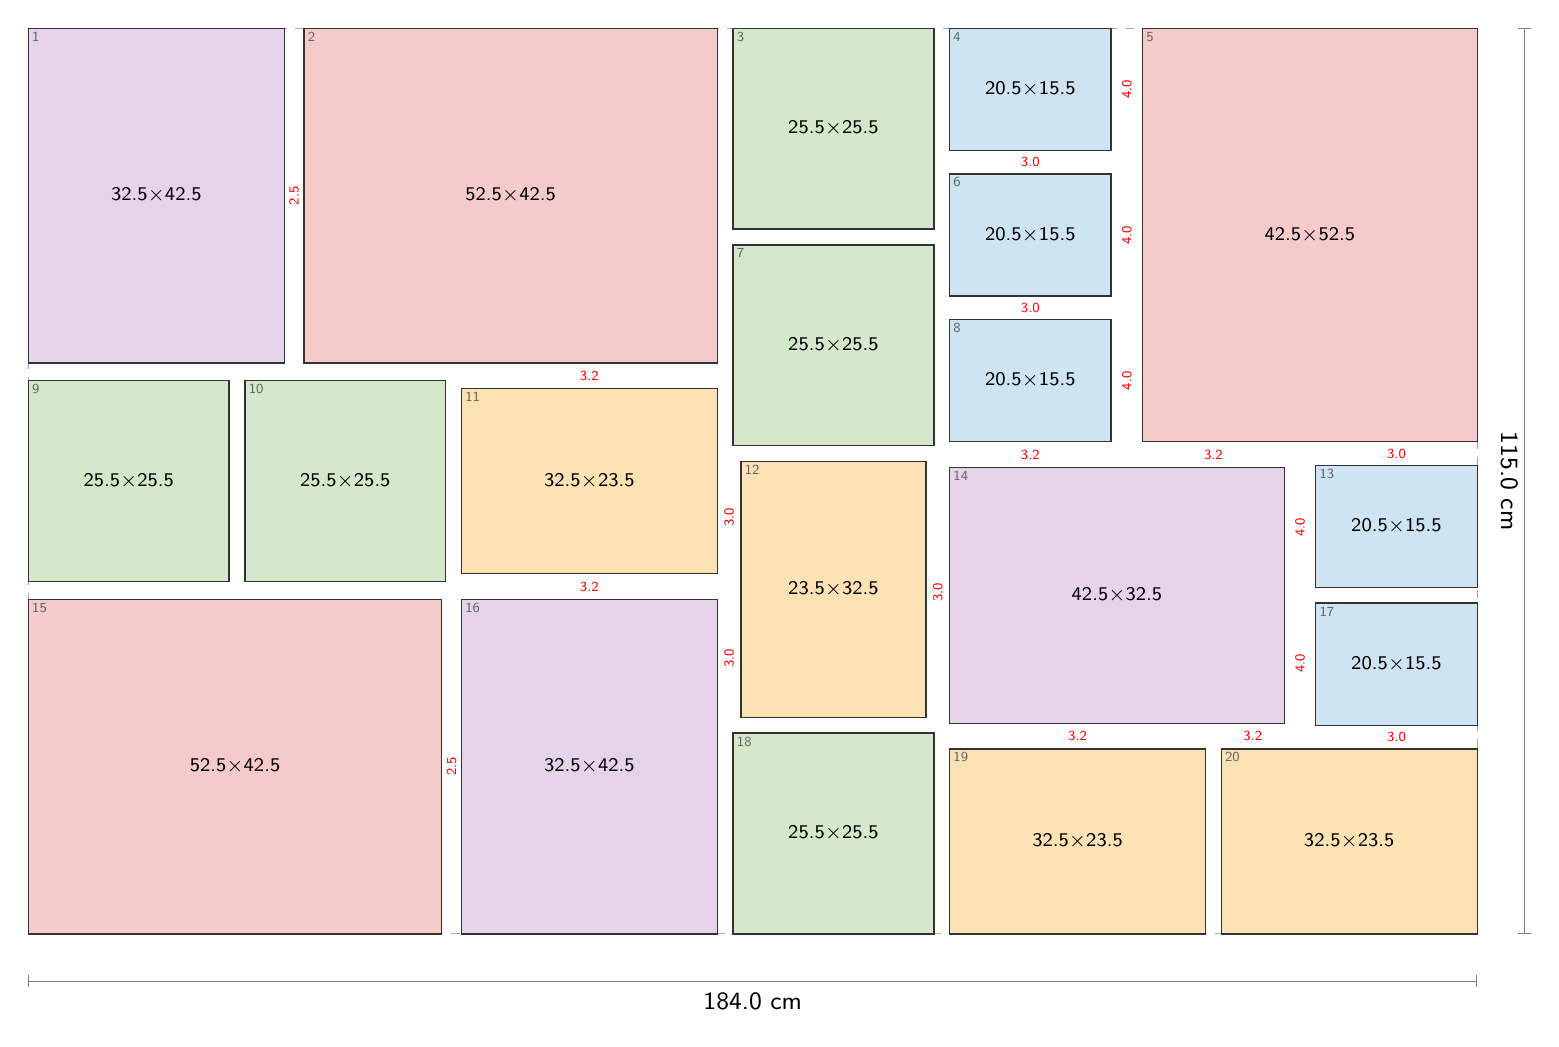
\begin{tikzpicture}[x=1mm, y=-1mm]
\draw[gray!70, dashed, line width=0.4pt] (0,0) rectangle (184.00,115.00);
\filldraw[fill=ft3, draw=black!80, line width=0.5pt] (0.00,0.00) rectangle (32.50,42.50);
\node[align=center, inner sep=0pt] at (16.25,21.25) {\scriptsize 32.5$\times$42.5};
\node[anchor=north west, inner sep=1.2pt, font=\tiny, text=black!60] at (0.00,0.00) {1};
\filldraw[fill=ft4, draw=black!80, line width=0.5pt] (35.00,0.00) rectangle (87.50,42.50);
\node[align=center, inner sep=0pt] at (61.25,21.25) {\scriptsize 52.5$\times$42.5};
\node[anchor=north west, inner sep=1.2pt, font=\tiny, text=black!60] at (35.00,0.00) {2};
\filldraw[fill=ft2, draw=black!80, line width=0.5pt] (89.50,0.00) rectangle (115.00,25.50);
\node[align=center, inner sep=0pt] at (102.25,12.75) {\scriptsize 25.5$\times$25.5};
\node[anchor=north west, inner sep=1.2pt, font=\tiny, text=black!60] at (89.50,0.00) {3};
\filldraw[fill=ft0, draw=black!80, line width=0.5pt] (117.00,0.00) rectangle (137.50,15.50);
\node[align=center, inner sep=0pt] at (127.25,7.75) {\scriptsize 20.5$\times$15.5};
\node[anchor=north west, inner sep=1.2pt, font=\tiny, text=black!60] at (117.00,0.00) {4};
\filldraw[fill=ft4, draw=black!80, line width=0.5pt] (141.50,0.00) rectangle (184.00,52.50);
\node[align=center, inner sep=0pt] at (162.75,26.25) {\scriptsize 42.5$\times$52.5};
\node[anchor=north west, inner sep=1.2pt, font=\tiny, text=black!60] at (141.50,0.00) {5};
\filldraw[fill=ft0, draw=black!80, line width=0.5pt] (117.00,18.50) rectangle (137.50,34.00);
\node[align=center, inner sep=0pt] at (127.25,26.25) {\scriptsize 20.5$\times$15.5};
\node[anchor=north west, inner sep=1.2pt, font=\tiny, text=black!60] at (117.00,18.50) {6};
\filldraw[fill=ft2, draw=black!80, line width=0.5pt] (89.50,27.50) rectangle (115.00,53.00);
\node[align=center, inner sep=0pt] at (102.25,40.25) {\scriptsize 25.5$\times$25.5};
\node[anchor=north west, inner sep=1.2pt, font=\tiny, text=black!60] at (89.50,27.50) {7};
\filldraw[fill=ft0, draw=black!80, line width=0.5pt] (117.00,37.00) rectangle (137.50,52.50);
\node[align=center, inner sep=0pt] at (127.25,44.75) {\scriptsize 20.5$\times$15.5};
\node[anchor=north west, inner sep=1.2pt, font=\tiny, text=black!60] at (117.00,37.00) {8};
\filldraw[fill=ft2, draw=black!80, line width=0.5pt] (0.00,44.75) rectangle (25.50,70.25);
\node[align=center, inner sep=0pt] at (12.75,57.50) {\scriptsize 25.5$\times$25.5};
\node[anchor=north west, inner sep=1.2pt, font=\tiny, text=black!60] at (0.00,44.75) {9};
\filldraw[fill=ft2, draw=black!80, line width=0.5pt] (27.50,44.75) rectangle (53.00,70.25);
\node[align=center, inner sep=0pt] at (40.25,57.50) {\scriptsize 25.5$\times$25.5};
\node[anchor=north west, inner sep=1.2pt, font=\tiny, text=black!60] at (27.50,44.75) {10};
\filldraw[fill=ft1, draw=black!80, line width=0.5pt] (55.00,45.75) rectangle (87.50,69.25);
\node[align=center, inner sep=0pt] at (71.25,57.50) {\scriptsize 32.5$\times$23.5};
\node[anchor=north west, inner sep=1.2pt, font=\tiny, text=black!60] at (55.00,45.75) {11};
\filldraw[fill=ft1, draw=black!80, line width=0.5pt] (90.50,55.00) rectangle (114.00,87.50);
\node[align=center, inner sep=0pt] at (102.25,71.25) {\scriptsize 23.5$\times$32.5};
\node[anchor=north west, inner sep=1.2pt, font=\tiny, text=black!60] at (90.50,55.00) {12};
\filldraw[fill=ft0, draw=black!80, line width=0.5pt] (163.50,55.50) rectangle (184.00,71.00);
\node[align=center, inner sep=0pt] at (173.75,63.25) {\scriptsize 20.5$\times$15.5};
\node[anchor=north west, inner sep=1.2pt, font=\tiny, text=black!60] at (163.50,55.50) {13};
\filldraw[fill=ft3, draw=black!80, line width=0.5pt] (117.00,55.75) rectangle (159.50,88.25);
\node[align=center, inner sep=0pt] at (138.25,72.00) {\scriptsize 42.5$\times$32.5};
\node[anchor=north west, inner sep=1.2pt, font=\tiny, text=black!60] at (117.00,55.75) {14};
\filldraw[fill=ft4, draw=black!80, line width=0.5pt] (0.00,72.50) rectangle (52.50,115.00);
\node[align=center, inner sep=0pt] at (26.25,93.75) {\scriptsize 52.5$\times$42.5};
\node[anchor=north west, inner sep=1.2pt, font=\tiny, text=black!60] at (0.00,72.50) {15};
\filldraw[fill=ft3, draw=black!80, line width=0.5pt] (55.00,72.50) rectangle (87.50,115.00);
\node[align=center, inner sep=0pt] at (71.25,93.75) {\scriptsize 32.5$\times$42.5};
\node[anchor=north west, inner sep=1.2pt, font=\tiny, text=black!60] at (55.00,72.50) {16};
\filldraw[fill=ft0, draw=black!80, line width=0.5pt] (163.50,73.00) rectangle (184.00,88.50);
\node[align=center, inner sep=0pt] at (173.75,80.75) {\scriptsize 20.5$\times$15.5};
\node[anchor=north west, inner sep=1.2pt, font=\tiny, text=black!60] at (163.50,73.00) {17};
\filldraw[fill=ft2, draw=black!80, line width=0.5pt] (89.50,89.50) rectangle (115.00,115.00);
\node[align=center, inner sep=0pt] at (102.25,102.25) {\scriptsize 25.5$\times$25.5};
\node[anchor=north west, inner sep=1.2pt, font=\tiny, text=black!60] at (89.50,89.50) {18};
\filldraw[fill=ft1, draw=black!80, line width=0.5pt] (117.00,91.50) rectangle (149.50,115.00);
\node[align=center, inner sep=0pt] at (133.25,103.25) {\scriptsize 32.5$\times$23.5};
\node[anchor=north west, inner sep=1.2pt, font=\tiny, text=black!60] at (117.00,91.50) {19};
\filldraw[fill=ft1, draw=black!80, line width=0.5pt] (151.50,91.50) rectangle (184.00,115.00);
\node[align=center, inner sep=0pt] at (167.75,103.25) {\scriptsize 32.5$\times$23.5};
\node[anchor=north west, inner sep=1.2pt, font=\tiny, text=black!60] at (151.50,91.50) {20};
\node[font=\tiny, text=red, fill=white, inner sep=0.3pt, rotate=90] at (33.75,21.25) {2.5};
\node[font=\tiny, text=red, fill=white, inner sep=0.3pt] at (71.25,44.12) {3.2};
\node[font=\tiny, text=red, fill=white, inner sep=0.3pt, rotate=90] at (139.50,7.75) {4.0};
\node[font=\tiny, text=red, fill=white, inner sep=0.3pt] at (127.25,17.00) {3.0};
\node[font=\tiny, text=red, fill=white, inner sep=0.3pt] at (173.75,54.00) {3.0};
\node[font=\tiny, text=red, fill=white, inner sep=0.3pt] at (150.50,54.12) {3.2};
\node[font=\tiny, text=red, fill=white, inner sep=0.3pt, rotate=90] at (139.50,26.25) {4.0};
\node[font=\tiny, text=red, fill=white, inner sep=0.3pt] at (127.25,35.50) {3.0};
\node[font=\tiny, text=red, fill=white, inner sep=0.3pt, rotate=90] at (139.50,44.75) {4.0};
\node[font=\tiny, text=red, fill=white, inner sep=0.3pt] at (127.25,54.12) {3.2};
\node[font=\tiny, text=red, fill=white, inner sep=0.3pt, rotate=90] at (89.00,62.12) {3.0};
\node[font=\tiny, text=red, fill=white, inner sep=0.3pt] at (71.25,70.88) {3.2};
\node[font=\tiny, text=red, fill=white, inner sep=0.3pt, rotate=90] at (115.50,71.62) {3.0};
\node[font=\tiny, text=red, fill=white, inner sep=0.3pt, rotate=90] at (161.50,63.38) {4.0};
\node[font=\tiny, text=red, fill=white, inner sep=0.3pt, rotate=90] at (161.50,80.62) {4.0};
\node[font=\tiny, text=red, fill=white, inner sep=0.3pt] at (133.25,89.88) {3.2};
\node[font=\tiny, text=red, fill=white, inner sep=0.3pt] at (155.50,89.88) {3.2};
\node[font=\tiny, text=red, fill=white, inner sep=0.3pt, rotate=90] at (53.75,93.75) {2.5};
\node[font=\tiny, text=red, fill=white, inner sep=0.3pt, rotate=90] at (89.00,80.00) {3.0};
\node[font=\tiny, text=red, fill=white, inner sep=0.3pt] at (173.75,90.00) {3.0};
\draw[Bar-Bar, gray] (0,121.00) -- (184.00,121.00) node[midway, below=1pt, font=\small, text=black] {184.0 cm};
\draw[Bar-Bar, gray] (190.00,0) -- (190.00,115.00) node[midway, right=1pt, font=\small, text=black, rotate=-90, anchor=north] {115.0 cm};
\end{tikzpicture}\\[4pt]
{\scriptsize Scale 1:10 (1 mm = 1 cm). Red numbers mark gaps that deviate from the nominal gap by more than 0.25 cm. Small grey numbers index the coordinate table.}
\end{minipage}\hfill
\begin{minipage}[t]{0.25\textwidth}\vspace{0pt}
\small
\begin{tabular}{@{}l l@{}}
\toprule
Outer size & 184.0 $\times$ 115.0 cm \\
Nominal gap & 2 cm \\
Actual gaps & 2.0 -- 4.0 cm \\
Max.\ deviation & 2.0 cm \\
Mean deviation & 0.65 cm \\
Border notches & top 4 cm \\
Corners filled & 4 / 4 \\
Frames used & 20 of 28 \\
Large frames & {\scriptsize 3, not touching, min.\ dist.\ 81 cm} \\
Entropy & 0.75 \\
\quad {\scriptsize mix / variety} & {\scriptsize 0.86 / 0.80} \\
\quad {\scriptsize stagger / lines} & {\scriptsize 0.59 / 0.75 (2 through)} \\
\bottomrule
\end{tabular}

\vspace{8pt}
\scriptsize
\begin{tabular}{@{}c l l r r@{}}
\toprule
 & outer w $\times$ h (cm) &  & used & have \\
\midrule
\tikz[baseline=-0.6ex]\fill[ft0,draw=black!60] (0,0) rectangle (1.2ex,1.2ex); & 20.5$\times$15.5 & L & 5 & 9 \\
\tikz[baseline=-0.6ex]\fill[ft0,draw=black!60] (0,0) rectangle (1.2ex,1.2ex); & 15.5$\times$20.5 & P & 0 & 2 \\
\tikz[baseline=-0.6ex]\fill[ft3,draw=black!60] (0,0) rectangle (1.2ex,1.2ex); & 32.5$\times$42.5 & P & 2 & 2 \\
\tikz[baseline=-0.6ex]\fill[ft3,draw=black!60] (0,0) rectangle (1.2ex,1.2ex); & 42.5$\times$32.5 & L & 1 & 1 \\
\tikz[baseline=-0.6ex]\fill[ft1,draw=black!60] (0,0) rectangle (1.2ex,1.2ex); & 32.5$\times$23.5 & L & 3 & 5 \\
\tikz[baseline=-0.6ex]\fill[ft1,draw=black!60] (0,0) rectangle (1.2ex,1.2ex); & 23.5$\times$32.5 & P & 1 & 1 \\
\tikz[baseline=-0.6ex]\fill[ft2,draw=black!60] (0,0) rectangle (1.2ex,1.2ex); & 25.5$\times$25.5 &  & 5 & 5 \\
\tikz[baseline=-0.6ex]\fill[ft4,draw=black!60] (0,0) rectangle (1.2ex,1.2ex); & 42.5$\times$52.5 & P & 1 & 1 \\
\tikz[baseline=-0.6ex]\fill[ft4,draw=black!60] (0,0) rectangle (1.2ex,1.2ex); & 52.5$\times$42.5 & L & 2 & 2 \\
\bottomrule
\end{tabular}

\vspace{8pt}
{\bfseries Positions} (top-left corner, cm)\\[2pt]
\tiny
\begin{tabular}{@{}r l r r@{}}
\toprule
\# & frame w $\times$ h & x & y \\
\midrule
1 & 32.5 $\times$ 42.5 & 0.0 & 0.0 \\
2 & 52.5 $\times$ 42.5 & 35.0 & 0.0 \\
3 & 25.5 $\times$ 25.5 & 89.5 & 0.0 \\
4 & 20.5 $\times$ 15.5 & 117.0 & 0.0 \\
5 & 42.5 $\times$ 52.5 & 141.5 & 0.0 \\
6 & 20.5 $\times$ 15.5 & 117.0 & 18.5 \\
7 & 25.5 $\times$ 25.5 & 89.5 & 27.5 \\
8 & 20.5 $\times$ 15.5 & 117.0 & 37.0 \\
9 & 25.5 $\times$ 25.5 & 0.0 & 44.8 \\
10 & 25.5 $\times$ 25.5 & 27.5 & 44.8 \\
11 & 32.5 $\times$ 23.5 & 55.0 & 45.8 \\
12 & 23.5 $\times$ 32.5 & 90.5 & 55.0 \\
13 & 20.5 $\times$ 15.5 & 163.5 & 55.5 \\
14 & 42.5 $\times$ 32.5 & 117.0 & 55.8 \\
15 & 52.5 $\times$ 42.5 & 0.0 & 72.5 \\
16 & 32.5 $\times$ 42.5 & 55.0 & 72.5 \\
17 & 20.5 $\times$ 15.5 & 163.5 & 73.0 \\
18 & 25.5 $\times$ 25.5 & 89.5 & 89.5 \\
19 & 32.5 $\times$ 23.5 & 117.0 & 91.5 \\
20 & 32.5 $\times$ 23.5 & 151.5 & 91.5 \\
\bottomrule
\end{tabular}
\end{minipage}
\clearpage

\begin{minipage}[t]{0.74\textwidth}\vspace{0pt}
{\LARGE\bfseries Layout 3}\hspace{1.5em}{\large 179.5 $\times$ 120.5 cm \quad gap 1.5 cm \quad 26 frames}\\[8pt]
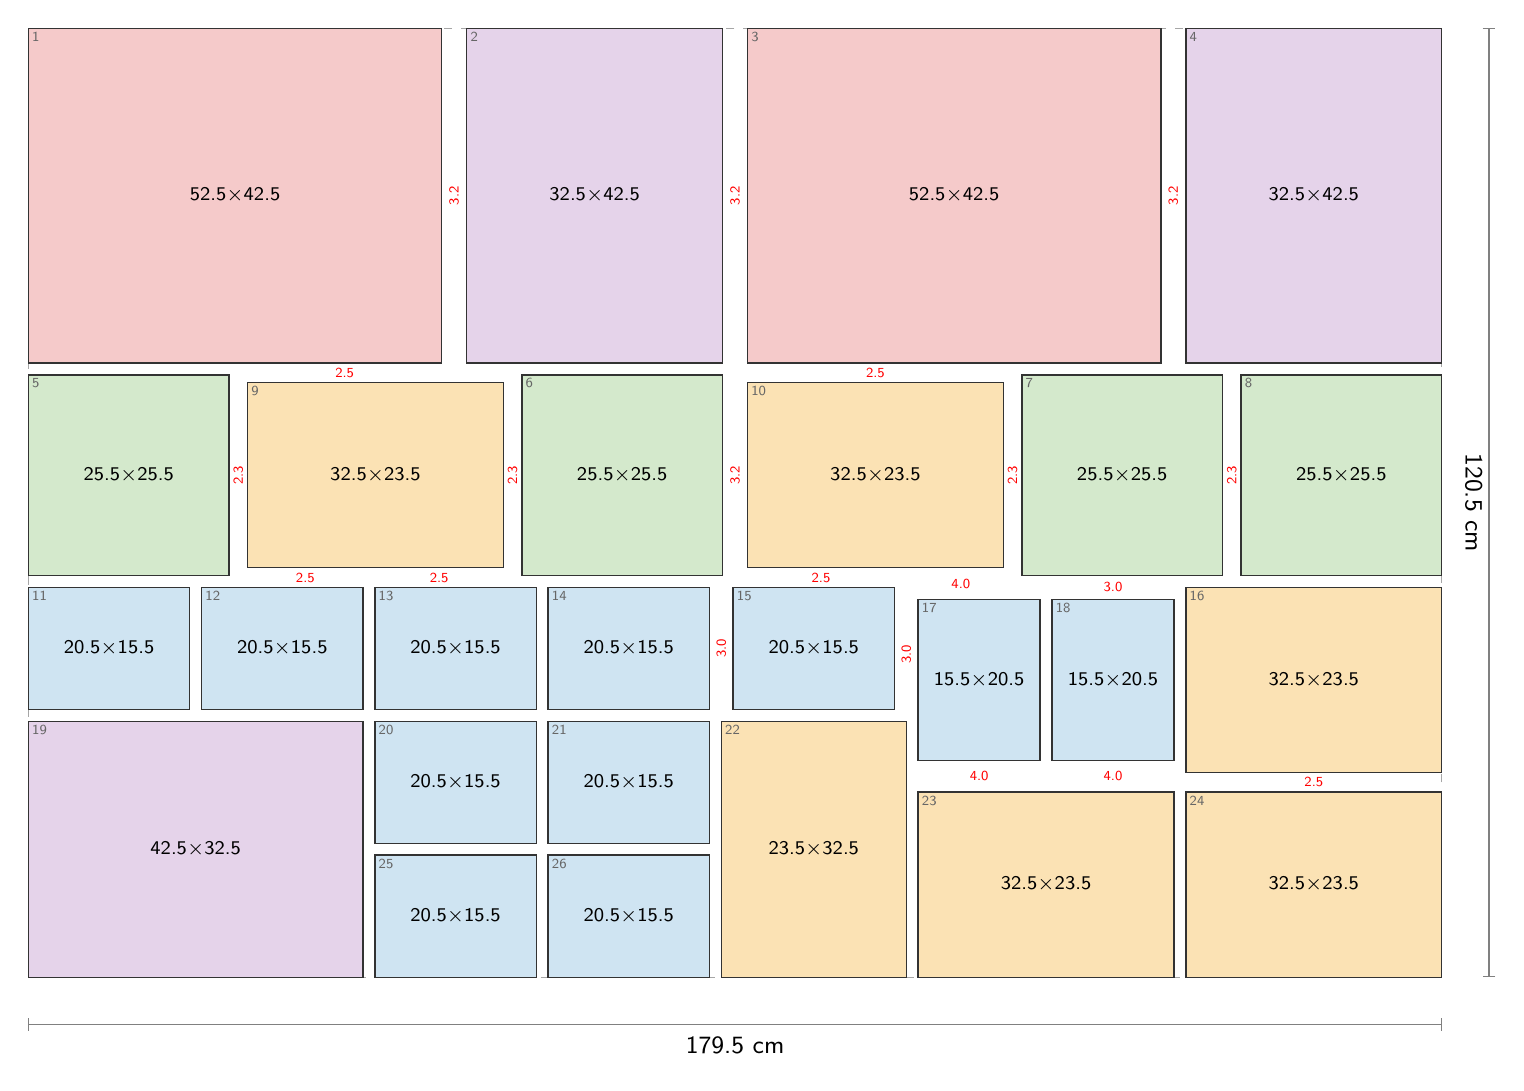
\begin{tikzpicture}[x=1mm, y=-1mm]
\draw[gray!70, dashed, line width=0.4pt] (0,0) rectangle (179.50,120.50);
\filldraw[fill=ft4, draw=black!80, line width=0.5pt] (0.00,0.00) rectangle (52.50,42.50);
\node[align=center, inner sep=0pt] at (26.25,21.25) {\scriptsize 52.5$\times$42.5};
\node[anchor=north west, inner sep=1.2pt, font=\tiny, text=black!60] at (0.00,0.00) {1};
\filldraw[fill=ft3, draw=black!80, line width=0.5pt] (55.67,0.00) rectangle (88.17,42.50);
\node[align=center, inner sep=0pt] at (71.92,21.25) {\scriptsize 32.5$\times$42.5};
\node[anchor=north west, inner sep=1.2pt, font=\tiny, text=black!60] at (55.67,0.00) {2};
\filldraw[fill=ft4, draw=black!80, line width=0.5pt] (91.33,0.00) rectangle (143.83,42.50);
\node[align=center, inner sep=0pt] at (117.58,21.25) {\scriptsize 52.5$\times$42.5};
\node[anchor=north west, inner sep=1.2pt, font=\tiny, text=black!60] at (91.33,0.00) {3};
\filldraw[fill=ft3, draw=black!80, line width=0.5pt] (147.00,0.00) rectangle (179.50,42.50);
\node[align=center, inner sep=0pt] at (163.25,21.25) {\scriptsize 32.5$\times$42.5};
\node[anchor=north west, inner sep=1.2pt, font=\tiny, text=black!60] at (147.00,0.00) {4};
\filldraw[fill=ft2, draw=black!80, line width=0.5pt] (0.00,44.00) rectangle (25.50,69.50);
\node[align=center, inner sep=0pt] at (12.75,56.75) {\scriptsize 25.5$\times$25.5};
\node[anchor=north west, inner sep=1.2pt, font=\tiny, text=black!60] at (0.00,44.00) {5};
\filldraw[fill=ft2, draw=black!80, line width=0.5pt] (62.67,44.00) rectangle (88.17,69.50);
\node[align=center, inner sep=0pt] at (75.42,56.75) {\scriptsize 25.5$\times$25.5};
\node[anchor=north west, inner sep=1.2pt, font=\tiny, text=black!60] at (62.67,44.00) {6};
\filldraw[fill=ft2, draw=black!80, line width=0.5pt] (126.17,44.00) rectangle (151.67,69.50);
\node[align=center, inner sep=0pt] at (138.92,56.75) {\scriptsize 25.5$\times$25.5};
\node[anchor=north west, inner sep=1.2pt, font=\tiny, text=black!60] at (126.17,44.00) {7};
\filldraw[fill=ft2, draw=black!80, line width=0.5pt] (154.00,44.00) rectangle (179.50,69.50);
\node[align=center, inner sep=0pt] at (166.75,56.75) {\scriptsize 25.5$\times$25.5};
\node[anchor=north west, inner sep=1.2pt, font=\tiny, text=black!60] at (154.00,44.00) {8};
\filldraw[fill=ft1, draw=black!80, line width=0.5pt] (27.83,45.00) rectangle (60.33,68.50);
\node[align=center, inner sep=0pt] at (44.08,56.75) {\scriptsize 32.5$\times$23.5};
\node[anchor=north west, inner sep=1.2pt, font=\tiny, text=black!60] at (27.83,45.00) {9};
\filldraw[fill=ft1, draw=black!80, line width=0.5pt] (91.33,45.00) rectangle (123.83,68.50);
\node[align=center, inner sep=0pt] at (107.58,56.75) {\scriptsize 32.5$\times$23.5};
\node[anchor=north west, inner sep=1.2pt, font=\tiny, text=black!60] at (91.33,45.00) {10};
\filldraw[fill=ft0, draw=black!80, line width=0.5pt] (0.00,71.00) rectangle (20.50,86.50);
\node[align=center, inner sep=0pt] at (10.25,78.75) {\scriptsize 20.5$\times$15.5};
\node[anchor=north west, inner sep=1.2pt, font=\tiny, text=black!60] at (0.00,71.00) {11};
\filldraw[fill=ft0, draw=black!80, line width=0.5pt] (22.00,71.00) rectangle (42.50,86.50);
\node[align=center, inner sep=0pt] at (32.25,78.75) {\scriptsize 20.5$\times$15.5};
\node[anchor=north west, inner sep=1.2pt, font=\tiny, text=black!60] at (22.00,71.00) {12};
\filldraw[fill=ft0, draw=black!80, line width=0.5pt] (44.00,71.00) rectangle (64.50,86.50);
\node[align=center, inner sep=0pt] at (54.25,78.75) {\scriptsize 20.5$\times$15.5};
\node[anchor=north west, inner sep=1.2pt, font=\tiny, text=black!60] at (44.00,71.00) {13};
\filldraw[fill=ft0, draw=black!80, line width=0.5pt] (66.00,71.00) rectangle (86.50,86.50);
\node[align=center, inner sep=0pt] at (76.25,78.75) {\scriptsize 20.5$\times$15.5};
\node[anchor=north west, inner sep=1.2pt, font=\tiny, text=black!60] at (66.00,71.00) {14};
\filldraw[fill=ft0, draw=black!80, line width=0.5pt] (89.50,71.00) rectangle (110.00,86.50);
\node[align=center, inner sep=0pt] at (99.75,78.75) {\scriptsize 20.5$\times$15.5};
\node[anchor=north west, inner sep=1.2pt, font=\tiny, text=black!60] at (89.50,71.00) {15};
\filldraw[fill=ft1, draw=black!80, line width=0.5pt] (147.00,71.00) rectangle (179.50,94.50);
\node[align=center, inner sep=0pt] at (163.25,82.75) {\scriptsize 32.5$\times$23.5};
\node[anchor=north west, inner sep=1.2pt, font=\tiny, text=black!60] at (147.00,71.00) {16};
\filldraw[fill=ft0, draw=black!80, line width=0.5pt] (113.00,72.50) rectangle (128.50,93.00);
\node[align=center, inner sep=0pt] at (120.75,82.75) {\scriptsize 15.5$\times$20.5};
\node[anchor=north west, inner sep=1.2pt, font=\tiny, text=black!60] at (113.00,72.50) {17};
\filldraw[fill=ft0, draw=black!80, line width=0.5pt] (130.00,72.50) rectangle (145.50,93.00);
\node[align=center, inner sep=0pt] at (137.75,82.75) {\scriptsize 15.5$\times$20.5};
\node[anchor=north west, inner sep=1.2pt, font=\tiny, text=black!60] at (130.00,72.50) {18};
\filldraw[fill=ft3, draw=black!80, line width=0.5pt] (0.00,88.00) rectangle (42.50,120.50);
\node[align=center, inner sep=0pt] at (21.25,104.25) {\scriptsize 42.5$\times$32.5};
\node[anchor=north west, inner sep=1.2pt, font=\tiny, text=black!60] at (0.00,88.00) {19};
\filldraw[fill=ft0, draw=black!80, line width=0.5pt] (44.00,88.00) rectangle (64.50,103.50);
\node[align=center, inner sep=0pt] at (54.25,95.75) {\scriptsize 20.5$\times$15.5};
\node[anchor=north west, inner sep=1.2pt, font=\tiny, text=black!60] at (44.00,88.00) {20};
\filldraw[fill=ft0, draw=black!80, line width=0.5pt] (66.00,88.00) rectangle (86.50,103.50);
\node[align=center, inner sep=0pt] at (76.25,95.75) {\scriptsize 20.5$\times$15.5};
\node[anchor=north west, inner sep=1.2pt, font=\tiny, text=black!60] at (66.00,88.00) {21};
\filldraw[fill=ft1, draw=black!80, line width=0.5pt] (88.00,88.00) rectangle (111.50,120.50);
\node[align=center, inner sep=0pt] at (99.75,104.25) {\scriptsize 23.5$\times$32.5};
\node[anchor=north west, inner sep=1.2pt, font=\tiny, text=black!60] at (88.00,88.00) {22};
\filldraw[fill=ft1, draw=black!80, line width=0.5pt] (113.00,97.00) rectangle (145.50,120.50);
\node[align=center, inner sep=0pt] at (129.25,108.75) {\scriptsize 32.5$\times$23.5};
\node[anchor=north west, inner sep=1.2pt, font=\tiny, text=black!60] at (113.00,97.00) {23};
\filldraw[fill=ft1, draw=black!80, line width=0.5pt] (147.00,97.00) rectangle (179.50,120.50);
\node[align=center, inner sep=0pt] at (163.25,108.75) {\scriptsize 32.5$\times$23.5};
\node[anchor=north west, inner sep=1.2pt, font=\tiny, text=black!60] at (147.00,97.00) {24};
\filldraw[fill=ft0, draw=black!80, line width=0.5pt] (44.00,105.00) rectangle (64.50,120.50);
\node[align=center, inner sep=0pt] at (54.25,112.75) {\scriptsize 20.5$\times$15.5};
\node[anchor=north west, inner sep=1.2pt, font=\tiny, text=black!60] at (44.00,105.00) {25};
\filldraw[fill=ft0, draw=black!80, line width=0.5pt] (66.00,105.00) rectangle (86.50,120.50);
\node[align=center, inner sep=0pt] at (76.25,112.75) {\scriptsize 20.5$\times$15.5};
\node[anchor=north west, inner sep=1.2pt, font=\tiny, text=black!60] at (66.00,105.00) {26};
\node[font=\tiny, text=red, fill=white, inner sep=0.3pt, rotate=90] at (54.08,21.25) {3.2};
\node[font=\tiny, text=red, fill=white, inner sep=0.3pt] at (40.17,43.75) {2.5};
\node[font=\tiny, text=red, fill=white, inner sep=0.3pt, rotate=90] at (89.75,21.25) {3.2};
\node[font=\tiny, text=red, fill=white, inner sep=0.3pt, rotate=90] at (145.42,21.25) {3.2};
\node[font=\tiny, text=red, fill=white, inner sep=0.3pt] at (107.58,43.75) {2.5};
\node[font=\tiny, text=red, fill=white, inner sep=0.3pt, rotate=90] at (26.67,56.75) {2.3};
\node[font=\tiny, text=red, fill=white, inner sep=0.3pt, rotate=90] at (89.75,56.75) {3.2};
\node[font=\tiny, text=red, fill=white, inner sep=0.3pt, rotate=90] at (152.83,56.75) {2.3};
\node[font=\tiny, text=red, fill=white, inner sep=0.3pt] at (137.75,71.00) {3.0};
\node[font=\tiny, text=red, fill=white, inner sep=0.3pt, rotate=90] at (61.50,56.75) {2.3};
\node[font=\tiny, text=red, fill=white, inner sep=0.3pt] at (35.17,69.75) {2.5};
\node[font=\tiny, text=red, fill=white, inner sep=0.3pt] at (52.17,69.75) {2.5};
\node[font=\tiny, text=red, fill=white, inner sep=0.3pt, rotate=90] at (125.00,56.75) {2.3};
\node[font=\tiny, text=red, fill=white, inner sep=0.3pt] at (100.67,69.75) {2.5};
\node[font=\tiny, text=red, fill=white, inner sep=0.3pt] at (118.42,70.50) {4.0};
\node[font=\tiny, text=red, fill=white, inner sep=0.3pt, rotate=90] at (88.00,78.75) {3.0};
\node[font=\tiny, text=red, fill=white, inner sep=0.3pt, rotate=90] at (111.50,79.50) {3.0};
\node[font=\tiny, text=red, fill=white, inner sep=0.3pt] at (163.25,95.75) {2.5};
\node[font=\tiny, text=red, fill=white, inner sep=0.3pt] at (120.75,95.00) {4.0};
\node[font=\tiny, text=red, fill=white, inner sep=0.3pt] at (137.75,95.00) {4.0};
\draw[Bar-Bar, gray] (0,126.50) -- (179.50,126.50) node[midway, below=1pt, font=\small, text=black] {179.5 cm};
\draw[Bar-Bar, gray] (185.50,0) -- (185.50,120.50) node[midway, right=1pt, font=\small, text=black, rotate=-90, anchor=north] {120.5 cm};
\end{tikzpicture}\\[4pt]
{\scriptsize Scale 1:10 (1 mm = 1 cm). Red numbers mark gaps that deviate from the nominal gap by more than 0.25 cm. Small grey numbers index the coordinate table.}
\end{minipage}\hfill
\begin{minipage}[t]{0.25\textwidth}\vspace{0pt}
\small
\begin{tabular}{@{}l l@{}}
\toprule
Outer size & 179.5 $\times$ 120.5 cm \\
Nominal gap & 1.5 cm \\
Actual gaps & 1.5 -- 4.0 cm \\
Max.\ deviation & 2.5 cm \\
Mean deviation & 0.58 cm \\
Border notches & top 10 cm \\
Corners filled & 4 / 4 \\
Frames used & 26 of 28 \\
Large frames & {\scriptsize 2, not touching, min.\ dist.\ 91 cm} \\
Entropy & 0.67 \\
\quad {\scriptsize mix / variety} & {\scriptsize 0.83 / 0.66} \\
\quad {\scriptsize stagger / lines} & {\scriptsize 0.45 / 0.75 (2 through)} \\
\bottomrule
\end{tabular}

\vspace{8pt}
\scriptsize
\begin{tabular}{@{}c l l r r@{}}
\toprule
 & outer w $\times$ h (cm) &  & used & have \\
\midrule
\tikz[baseline=-0.6ex]\fill[ft0,draw=black!60] (0,0) rectangle (1.2ex,1.2ex); & 20.5$\times$15.5 & L & 9 & 9 \\
\tikz[baseline=-0.6ex]\fill[ft0,draw=black!60] (0,0) rectangle (1.2ex,1.2ex); & 15.5$\times$20.5 & P & 2 & 2 \\
\tikz[baseline=-0.6ex]\fill[ft3,draw=black!60] (0,0) rectangle (1.2ex,1.2ex); & 32.5$\times$42.5 & P & 2 & 2 \\
\tikz[baseline=-0.6ex]\fill[ft3,draw=black!60] (0,0) rectangle (1.2ex,1.2ex); & 42.5$\times$32.5 & L & 1 & 1 \\
\tikz[baseline=-0.6ex]\fill[ft1,draw=black!60] (0,0) rectangle (1.2ex,1.2ex); & 32.5$\times$23.5 & L & 5 & 5 \\
\tikz[baseline=-0.6ex]\fill[ft1,draw=black!60] (0,0) rectangle (1.2ex,1.2ex); & 23.5$\times$32.5 & P & 1 & 1 \\
\tikz[baseline=-0.6ex]\fill[ft2,draw=black!60] (0,0) rectangle (1.2ex,1.2ex); & 25.5$\times$25.5 &  & 4 & 5 \\
\tikz[baseline=-0.6ex]\fill[ft4,draw=black!60] (0,0) rectangle (1.2ex,1.2ex); & 42.5$\times$52.5 & P & 0 & 1 \\
\tikz[baseline=-0.6ex]\fill[ft4,draw=black!60] (0,0) rectangle (1.2ex,1.2ex); & 52.5$\times$42.5 & L & 2 & 2 \\
\bottomrule
\end{tabular}

\vspace{8pt}
{\bfseries Positions} (top-left corner, cm)\\[2pt]
\tiny
\begin{tabular}{@{}r l r r@{}}
\toprule
\# & frame w $\times$ h & x & y \\
\midrule
1 & 52.5 $\times$ 42.5 & 0.0 & 0.0 \\
2 & 32.5 $\times$ 42.5 & 55.7 & 0.0 \\
3 & 52.5 $\times$ 42.5 & 91.3 & 0.0 \\
4 & 32.5 $\times$ 42.5 & 147.0 & 0.0 \\
5 & 25.5 $\times$ 25.5 & 0.0 & 44.0 \\
6 & 25.5 $\times$ 25.5 & 62.7 & 44.0 \\
7 & 25.5 $\times$ 25.5 & 126.2 & 44.0 \\
8 & 25.5 $\times$ 25.5 & 154.0 & 44.0 \\
9 & 32.5 $\times$ 23.5 & 27.8 & 45.0 \\
10 & 32.5 $\times$ 23.5 & 91.3 & 45.0 \\
11 & 20.5 $\times$ 15.5 & 0.0 & 71.0 \\
12 & 20.5 $\times$ 15.5 & 22.0 & 71.0 \\
13 & 20.5 $\times$ 15.5 & 44.0 & 71.0 \\
14 & 20.5 $\times$ 15.5 & 66.0 & 71.0 \\
15 & 20.5 $\times$ 15.5 & 89.5 & 71.0 \\
16 & 32.5 $\times$ 23.5 & 147.0 & 71.0 \\
17 & 15.5 $\times$ 20.5 & 113.0 & 72.5 \\
18 & 15.5 $\times$ 20.5 & 130.0 & 72.5 \\
19 & 42.5 $\times$ 32.5 & 0.0 & 88.0 \\
20 & 20.5 $\times$ 15.5 & 44.0 & 88.0 \\
21 & 20.5 $\times$ 15.5 & 66.0 & 88.0 \\
22 & 23.5 $\times$ 32.5 & 88.0 & 88.0 \\
23 & 32.5 $\times$ 23.5 & 113.0 & 97.0 \\
24 & 32.5 $\times$ 23.5 & 147.0 & 97.0 \\
25 & 20.5 $\times$ 15.5 & 44.0 & 105.0 \\
26 & 20.5 $\times$ 15.5 & 66.0 & 105.0 \\
\bottomrule
\end{tabular}
\end{minipage}
\clearpage

\begin{minipage}[t]{0.74\textwidth}\vspace{0pt}
{\LARGE\bfseries Layout 4}\hspace{1.5em}{\large 172.5 $\times$ 125.5 cm \quad gap 2.5 cm \quad 25 frames}\\[8pt]
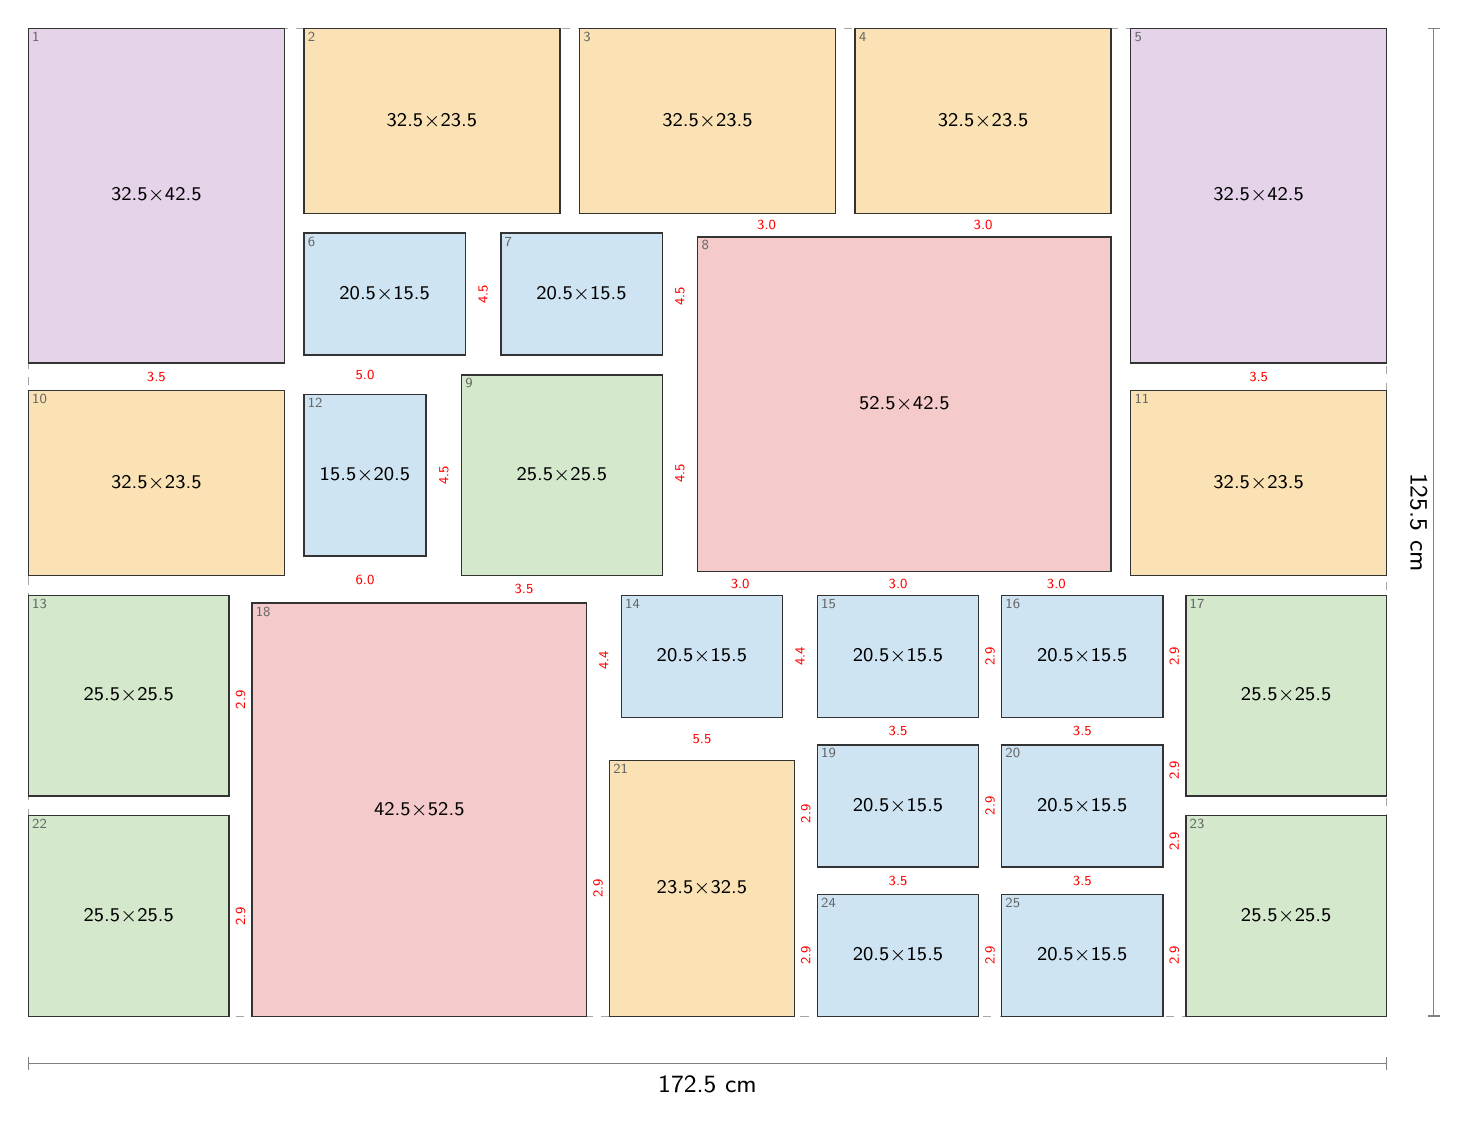
\begin{tikzpicture}[x=1mm, y=-1mm]
\draw[gray!70, dashed, line width=0.4pt] (0,0) rectangle (172.50,125.50);
\filldraw[fill=ft3, draw=black!80, line width=0.5pt] (0.00,0.00) rectangle (32.50,42.50);
\node[align=center, inner sep=0pt] at (16.25,21.25) {\scriptsize 32.5$\times$42.5};
\node[anchor=north west, inner sep=1.2pt, font=\tiny, text=black!60] at (0.00,0.00) {1};
\filldraw[fill=ft1, draw=black!80, line width=0.5pt] (35.00,0.00) rectangle (67.50,23.50);
\node[align=center, inner sep=0pt] at (51.25,11.75) {\scriptsize 32.5$\times$23.5};
\node[anchor=north west, inner sep=1.2pt, font=\tiny, text=black!60] at (35.00,0.00) {2};
\filldraw[fill=ft1, draw=black!80, line width=0.5pt] (70.00,0.00) rectangle (102.50,23.50);
\node[align=center, inner sep=0pt] at (86.25,11.75) {\scriptsize 32.5$\times$23.5};
\node[anchor=north west, inner sep=1.2pt, font=\tiny, text=black!60] at (70.00,0.00) {3};
\filldraw[fill=ft1, draw=black!80, line width=0.5pt] (105.00,0.00) rectangle (137.50,23.50);
\node[align=center, inner sep=0pt] at (121.25,11.75) {\scriptsize 32.5$\times$23.5};
\node[anchor=north west, inner sep=1.2pt, font=\tiny, text=black!60] at (105.00,0.00) {4};
\filldraw[fill=ft3, draw=black!80, line width=0.5pt] (140.00,0.00) rectangle (172.50,42.50);
\node[align=center, inner sep=0pt] at (156.25,21.25) {\scriptsize 32.5$\times$42.5};
\node[anchor=north west, inner sep=1.2pt, font=\tiny, text=black!60] at (140.00,0.00) {5};
\filldraw[fill=ft0, draw=black!80, line width=0.5pt] (35.00,26.00) rectangle (55.50,41.50);
\node[align=center, inner sep=0pt] at (45.25,33.75) {\scriptsize 20.5$\times$15.5};
\node[anchor=north west, inner sep=1.2pt, font=\tiny, text=black!60] at (35.00,26.00) {6};
\filldraw[fill=ft0, draw=black!80, line width=0.5pt] (60.00,26.00) rectangle (80.50,41.50);
\node[align=center, inner sep=0pt] at (70.25,33.75) {\scriptsize 20.5$\times$15.5};
\node[anchor=north west, inner sep=1.2pt, font=\tiny, text=black!60] at (60.00,26.00) {7};
\filldraw[fill=ft4, draw=black!80, line width=0.5pt] (85.00,26.50) rectangle (137.50,69.00);
\node[align=center, inner sep=0pt] at (111.25,47.75) {\scriptsize 52.5$\times$42.5};
\node[anchor=north west, inner sep=1.2pt, font=\tiny, text=black!60] at (85.00,26.50) {8};
\filldraw[fill=ft2, draw=black!80, line width=0.5pt] (55.00,44.00) rectangle (80.50,69.50);
\node[align=center, inner sep=0pt] at (67.75,56.75) {\scriptsize 25.5$\times$25.5};
\node[anchor=north west, inner sep=1.2pt, font=\tiny, text=black!60] at (55.00,44.00) {9};
\filldraw[fill=ft1, draw=black!80, line width=0.5pt] (0.00,46.00) rectangle (32.50,69.50);
\node[align=center, inner sep=0pt] at (16.25,57.75) {\scriptsize 32.5$\times$23.5};
\node[anchor=north west, inner sep=1.2pt, font=\tiny, text=black!60] at (0.00,46.00) {10};
\filldraw[fill=ft1, draw=black!80, line width=0.5pt] (140.00,46.00) rectangle (172.50,69.50);
\node[align=center, inner sep=0pt] at (156.25,57.75) {\scriptsize 32.5$\times$23.5};
\node[anchor=north west, inner sep=1.2pt, font=\tiny, text=black!60] at (140.00,46.00) {11};
\filldraw[fill=ft0, draw=black!80, line width=0.5pt] (35.00,46.50) rectangle (50.50,67.00);
\node[align=center, inner sep=0pt] at (42.75,56.75) {\scriptsize 15.5$\times$20.5};
\node[anchor=north west, inner sep=1.2pt, font=\tiny, text=black!60] at (35.00,46.50) {12};
\filldraw[fill=ft2, draw=black!80, line width=0.5pt] (0.00,72.00) rectangle (25.50,97.50);
\node[align=center, inner sep=0pt] at (12.75,84.75) {\scriptsize 25.5$\times$25.5};
\node[anchor=north west, inner sep=1.2pt, font=\tiny, text=black!60] at (0.00,72.00) {13};
\filldraw[fill=ft0, draw=black!80, line width=0.5pt] (75.30,72.00) rectangle (95.80,87.50);
\node[align=center, inner sep=0pt] at (85.55,79.75) {\scriptsize 20.5$\times$15.5};
\node[anchor=north west, inner sep=1.2pt, font=\tiny, text=black!60] at (75.30,72.00) {14};
\filldraw[fill=ft0, draw=black!80, line width=0.5pt] (100.20,72.00) rectangle (120.70,87.50);
\node[align=center, inner sep=0pt] at (110.45,79.75) {\scriptsize 20.5$\times$15.5};
\node[anchor=north west, inner sep=1.2pt, font=\tiny, text=black!60] at (100.20,72.00) {15};
\filldraw[fill=ft0, draw=black!80, line width=0.5pt] (123.60,72.00) rectangle (144.10,87.50);
\node[align=center, inner sep=0pt] at (133.85,79.75) {\scriptsize 20.5$\times$15.5};
\node[anchor=north west, inner sep=1.2pt, font=\tiny, text=black!60] at (123.60,72.00) {16};
\filldraw[fill=ft2, draw=black!80, line width=0.5pt] (147.00,72.00) rectangle (172.50,97.50);
\node[align=center, inner sep=0pt] at (159.75,84.75) {\scriptsize 25.5$\times$25.5};
\node[anchor=north west, inner sep=1.2pt, font=\tiny, text=black!60] at (147.00,72.00) {17};
\filldraw[fill=ft4, draw=black!80, line width=0.5pt] (28.40,73.00) rectangle (70.90,125.50);
\node[align=center, inner sep=0pt] at (49.65,99.25) {\scriptsize 42.5$\times$52.5};
\node[anchor=north west, inner sep=1.2pt, font=\tiny, text=black!60] at (28.40,73.00) {18};
\filldraw[fill=ft0, draw=black!80, line width=0.5pt] (100.20,91.00) rectangle (120.70,106.50);
\node[align=center, inner sep=0pt] at (110.45,98.75) {\scriptsize 20.5$\times$15.5};
\node[anchor=north west, inner sep=1.2pt, font=\tiny, text=black!60] at (100.20,91.00) {19};
\filldraw[fill=ft0, draw=black!80, line width=0.5pt] (123.60,91.00) rectangle (144.10,106.50);
\node[align=center, inner sep=0pt] at (133.85,98.75) {\scriptsize 20.5$\times$15.5};
\node[anchor=north west, inner sep=1.2pt, font=\tiny, text=black!60] at (123.60,91.00) {20};
\filldraw[fill=ft1, draw=black!80, line width=0.5pt] (73.80,93.00) rectangle (97.30,125.50);
\node[align=center, inner sep=0pt] at (85.55,109.25) {\scriptsize 23.5$\times$32.5};
\node[anchor=north west, inner sep=1.2pt, font=\tiny, text=black!60] at (73.80,93.00) {21};
\filldraw[fill=ft2, draw=black!80, line width=0.5pt] (0.00,100.00) rectangle (25.50,125.50);
\node[align=center, inner sep=0pt] at (12.75,112.75) {\scriptsize 25.5$\times$25.5};
\node[anchor=north west, inner sep=1.2pt, font=\tiny, text=black!60] at (0.00,100.00) {22};
\filldraw[fill=ft2, draw=black!80, line width=0.5pt] (147.00,100.00) rectangle (172.50,125.50);
\node[align=center, inner sep=0pt] at (159.75,112.75) {\scriptsize 25.5$\times$25.5};
\node[anchor=north west, inner sep=1.2pt, font=\tiny, text=black!60] at (147.00,100.00) {23};
\filldraw[fill=ft0, draw=black!80, line width=0.5pt] (100.20,110.00) rectangle (120.70,125.50);
\node[align=center, inner sep=0pt] at (110.45,117.75) {\scriptsize 20.5$\times$15.5};
\node[anchor=north west, inner sep=1.2pt, font=\tiny, text=black!60] at (100.20,110.00) {24};
\filldraw[fill=ft0, draw=black!80, line width=0.5pt] (123.60,110.00) rectangle (144.10,125.50);
\node[align=center, inner sep=0pt] at (133.85,117.75) {\scriptsize 20.5$\times$15.5};
\node[anchor=north west, inner sep=1.2pt, font=\tiny, text=black!60] at (123.60,110.00) {25};
\node[font=\tiny, text=red, fill=white, inner sep=0.3pt] at (16.25,44.25) {3.5};
\node[font=\tiny, text=red, fill=white, inner sep=0.3pt] at (93.75,25.00) {3.0};
\node[font=\tiny, text=red, fill=white, inner sep=0.3pt] at (121.25,25.00) {3.0};
\node[font=\tiny, text=red, fill=white, inner sep=0.3pt] at (156.25,44.25) {3.5};
\node[font=\tiny, text=red, fill=white, inner sep=0.3pt, rotate=90] at (57.75,33.75) {4.5};
\node[font=\tiny, text=red, fill=white, inner sep=0.3pt] at (42.75,44.00) {5.0};
\node[font=\tiny, text=red, fill=white, inner sep=0.3pt, rotate=90] at (82.75,34.00) {4.5};
\node[font=\tiny, text=red, fill=white, inner sep=0.3pt] at (90.40,70.50) {3.0};
\node[font=\tiny, text=red, fill=white, inner sep=0.3pt] at (110.45,70.50) {3.0};
\node[font=\tiny, text=red, fill=white, inner sep=0.3pt] at (130.55,70.50) {3.0};
\node[font=\tiny, text=red, fill=white, inner sep=0.3pt, rotate=90] at (82.75,56.50) {4.5};
\node[font=\tiny, text=red, fill=white, inner sep=0.3pt] at (62.95,71.25) {3.5};
\node[font=\tiny, text=red, fill=white, inner sep=0.3pt, rotate=90] at (52.75,56.75) {4.5};
\node[font=\tiny, text=red, fill=white, inner sep=0.3pt] at (42.75,70.00) {6.0};
\node[font=\tiny, text=red, fill=white, inner sep=0.3pt, rotate=90] at (26.95,85.25) {2.9};
\node[font=\tiny, text=red, fill=white, inner sep=0.3pt, rotate=90] at (98.00,79.75) {4.4};
\node[font=\tiny, text=red, fill=white, inner sep=0.3pt] at (85.55,90.25) {5.5};
\node[font=\tiny, text=red, fill=white, inner sep=0.3pt, rotate=90] at (122.15,79.75) {2.9};
\node[font=\tiny, text=red, fill=white, inner sep=0.3pt] at (110.45,89.25) {3.5};
\node[font=\tiny, text=red, fill=white, inner sep=0.3pt, rotate=90] at (145.55,79.75) {2.9};
\node[font=\tiny, text=red, fill=white, inner sep=0.3pt] at (133.85,89.25) {3.5};
\node[font=\tiny, text=red, fill=white, inner sep=0.3pt, rotate=90] at (73.10,80.25) {4.4};
\node[font=\tiny, text=red, fill=white, inner sep=0.3pt, rotate=90] at (72.35,109.25) {2.9};
\node[font=\tiny, text=red, fill=white, inner sep=0.3pt, rotate=90] at (122.15,98.75) {2.9};
\node[font=\tiny, text=red, fill=white, inner sep=0.3pt] at (110.45,108.25) {3.5};
\node[font=\tiny, text=red, fill=white, inner sep=0.3pt, rotate=90] at (145.55,94.25) {2.9};
\node[font=\tiny, text=red, fill=white, inner sep=0.3pt, rotate=90] at (145.55,103.25) {2.9};
\node[font=\tiny, text=red, fill=white, inner sep=0.3pt] at (133.85,108.25) {3.5};
\node[font=\tiny, text=red, fill=white, inner sep=0.3pt, rotate=90] at (98.75,99.75) {2.9};
\node[font=\tiny, text=red, fill=white, inner sep=0.3pt, rotate=90] at (98.75,117.75) {2.9};
\node[font=\tiny, text=red, fill=white, inner sep=0.3pt, rotate=90] at (26.95,112.75) {2.9};
\node[font=\tiny, text=red, fill=white, inner sep=0.3pt, rotate=90] at (122.15,117.75) {2.9};
\node[font=\tiny, text=red, fill=white, inner sep=0.3pt, rotate=90] at (145.55,117.75) {2.9};
\draw[Bar-Bar, gray] (0,131.50) -- (172.50,131.50) node[midway, below=1pt, font=\small, text=black] {172.5 cm};
\draw[Bar-Bar, gray] (178.50,0) -- (178.50,125.50) node[midway, right=1pt, font=\small, text=black, rotate=-90, anchor=north] {125.5 cm};
\end{tikzpicture}\\[4pt]
{\scriptsize Scale 1:10 (1 mm = 1 cm). Red numbers mark gaps that deviate from the nominal gap by more than 0.25 cm. Small grey numbers index the coordinate table.}
\end{minipage}\hfill
\begin{minipage}[t]{0.25\textwidth}\vspace{0pt}
\small
\begin{tabular}{@{}l l@{}}
\toprule
Outer size & 172.5 $\times$ 125.5 cm \\
Nominal gap & 2.5 cm \\
Actual gaps & 2.5 -- 6.0 cm \\
Max.\ deviation & 3.5 cm \\
Mean deviation & 0.70 cm \\
Border notches & none \\
Corners filled & 4 / 4 \\
Frames used & 25 of 28 \\
Large frames & {\scriptsize 2, not touching, min.\ dist.\ 80 cm} \\
Entropy & 0.75 \\
\quad {\scriptsize mix / variety} & {\scriptsize 0.79 / 0.73} \\
\quad {\scriptsize stagger / lines} & {\scriptsize 0.50 / 1.00 (1 through)} \\
\bottomrule
\end{tabular}

\vspace{8pt}
\scriptsize
\begin{tabular}{@{}c l l r r@{}}
\toprule
 & outer w $\times$ h (cm) &  & used & have \\
\midrule
\tikz[baseline=-0.6ex]\fill[ft0,draw=black!60] (0,0) rectangle (1.2ex,1.2ex); & 20.5$\times$15.5 & L & 9 & 9 \\
\tikz[baseline=-0.6ex]\fill[ft0,draw=black!60] (0,0) rectangle (1.2ex,1.2ex); & 15.5$\times$20.5 & P & 1 & 2 \\
\tikz[baseline=-0.6ex]\fill[ft3,draw=black!60] (0,0) rectangle (1.2ex,1.2ex); & 32.5$\times$42.5 & P & 2 & 2 \\
\tikz[baseline=-0.6ex]\fill[ft3,draw=black!60] (0,0) rectangle (1.2ex,1.2ex); & 42.5$\times$32.5 & L & 0 & 1 \\
\tikz[baseline=-0.6ex]\fill[ft1,draw=black!60] (0,0) rectangle (1.2ex,1.2ex); & 32.5$\times$23.5 & L & 5 & 5 \\
\tikz[baseline=-0.6ex]\fill[ft1,draw=black!60] (0,0) rectangle (1.2ex,1.2ex); & 23.5$\times$32.5 & P & 1 & 1 \\
\tikz[baseline=-0.6ex]\fill[ft2,draw=black!60] (0,0) rectangle (1.2ex,1.2ex); & 25.5$\times$25.5 &  & 5 & 5 \\
\tikz[baseline=-0.6ex]\fill[ft4,draw=black!60] (0,0) rectangle (1.2ex,1.2ex); & 42.5$\times$52.5 & P & 1 & 1 \\
\tikz[baseline=-0.6ex]\fill[ft4,draw=black!60] (0,0) rectangle (1.2ex,1.2ex); & 52.5$\times$42.5 & L & 1 & 2 \\
\bottomrule
\end{tabular}

\vspace{8pt}
{\bfseries Positions} (top-left corner, cm)\\[2pt]
\tiny
\begin{tabular}{@{}r l r r@{}}
\toprule
\# & frame w $\times$ h & x & y \\
\midrule
1 & 32.5 $\times$ 42.5 & 0.0 & 0.0 \\
2 & 32.5 $\times$ 23.5 & 35.0 & 0.0 \\
3 & 32.5 $\times$ 23.5 & 70.0 & 0.0 \\
4 & 32.5 $\times$ 23.5 & 105.0 & 0.0 \\
5 & 32.5 $\times$ 42.5 & 140.0 & 0.0 \\
6 & 20.5 $\times$ 15.5 & 35.0 & 26.0 \\
7 & 20.5 $\times$ 15.5 & 60.0 & 26.0 \\
8 & 52.5 $\times$ 42.5 & 85.0 & 26.5 \\
9 & 25.5 $\times$ 25.5 & 55.0 & 44.0 \\
10 & 32.5 $\times$ 23.5 & 0.0 & 46.0 \\
11 & 32.5 $\times$ 23.5 & 140.0 & 46.0 \\
12 & 15.5 $\times$ 20.5 & 35.0 & 46.5 \\
13 & 25.5 $\times$ 25.5 & 0.0 & 72.0 \\
14 & 20.5 $\times$ 15.5 & 75.3 & 72.0 \\
15 & 20.5 $\times$ 15.5 & 100.2 & 72.0 \\
16 & 20.5 $\times$ 15.5 & 123.6 & 72.0 \\
17 & 25.5 $\times$ 25.5 & 147.0 & 72.0 \\
18 & 42.5 $\times$ 52.5 & 28.4 & 73.0 \\
19 & 20.5 $\times$ 15.5 & 100.2 & 91.0 \\
20 & 20.5 $\times$ 15.5 & 123.6 & 91.0 \\
21 & 23.5 $\times$ 32.5 & 73.8 & 93.0 \\
22 & 25.5 $\times$ 25.5 & 0.0 & 100.0 \\
23 & 25.5 $\times$ 25.5 & 147.0 & 100.0 \\
24 & 20.5 $\times$ 15.5 & 100.2 & 110.0 \\
25 & 20.5 $\times$ 15.5 & 123.6 & 110.0 \\
\bottomrule
\end{tabular}
\end{minipage}
\clearpage

\begin{minipage}[t]{0.74\textwidth}\vspace{0pt}
{\LARGE\bfseries Layout 5}\hspace{1.5em}{\large 174.5 $\times$ 130.5 cm \quad gap 1.5 cm \quad 25 frames}\\[8pt]
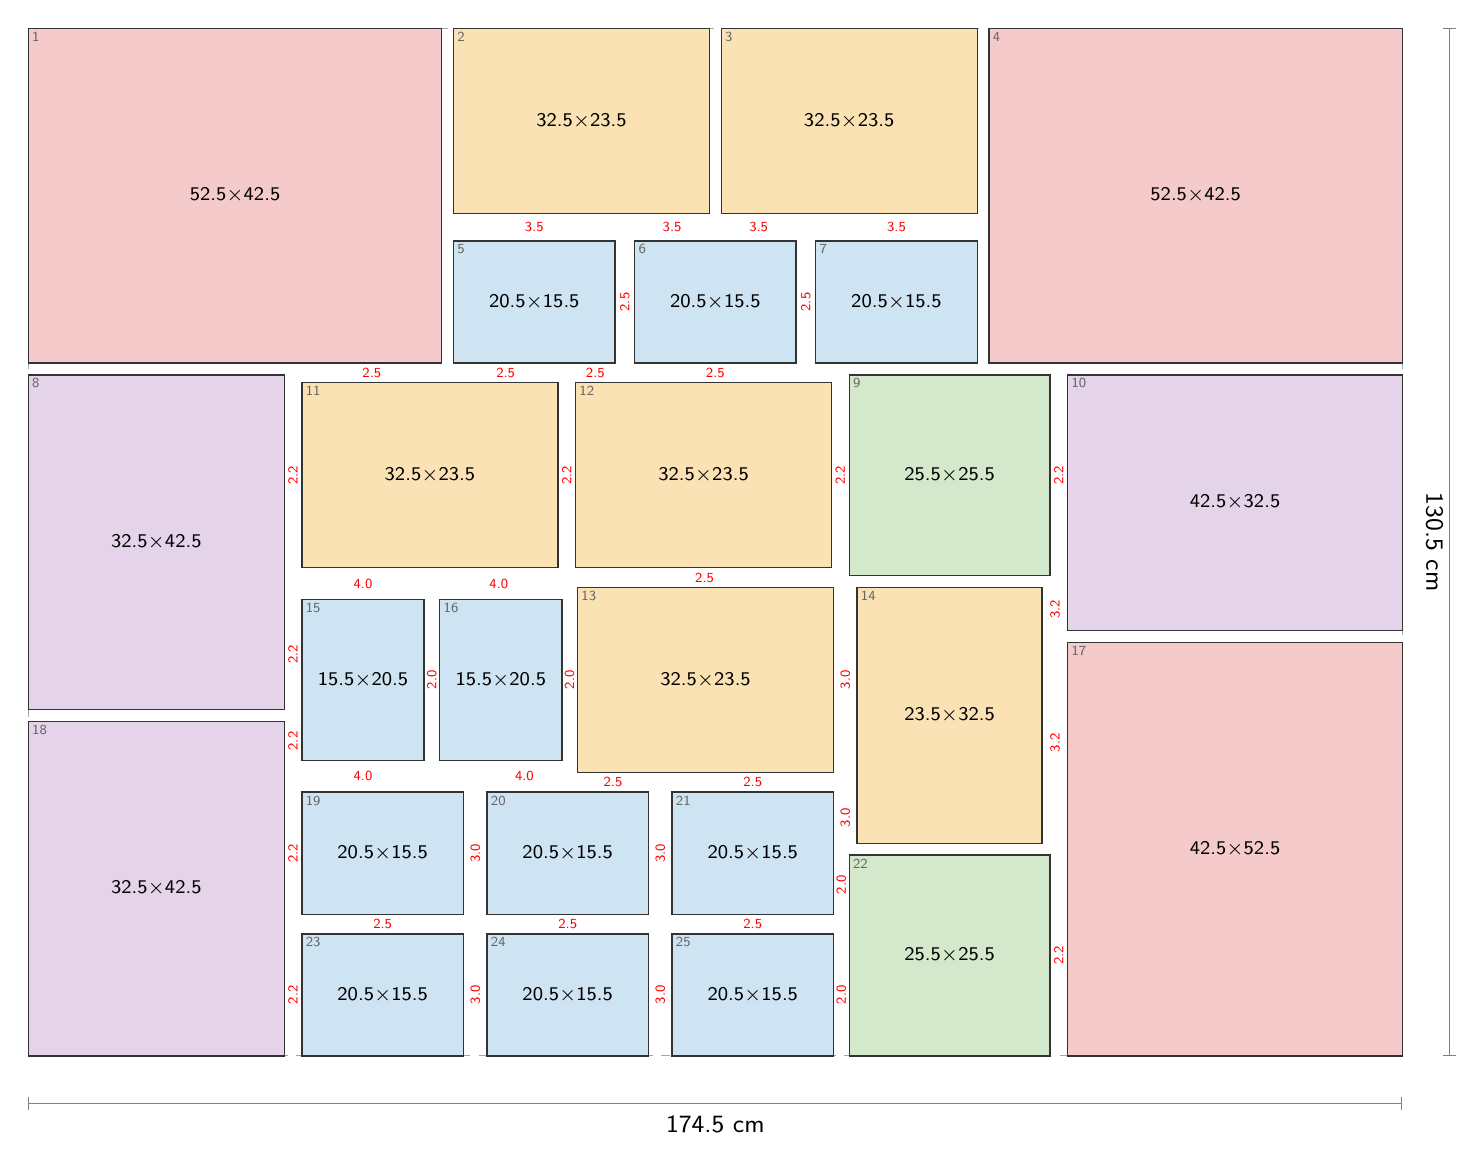
\begin{tikzpicture}[x=1mm, y=-1mm]
\draw[gray!70, dashed, line width=0.4pt] (0,0) rectangle (174.50,130.50);
\filldraw[fill=ft4, draw=black!80, line width=0.5pt] (0.00,0.00) rectangle (52.50,42.50);
\node[align=center, inner sep=0pt] at (26.25,21.25) {\scriptsize 52.5$\times$42.5};
\node[anchor=north west, inner sep=1.2pt, font=\tiny, text=black!60] at (0.00,0.00) {1};
\filldraw[fill=ft1, draw=black!80, line width=0.5pt] (54.00,0.00) rectangle (86.50,23.50);
\node[align=center, inner sep=0pt] at (70.25,11.75) {\scriptsize 32.5$\times$23.5};
\node[anchor=north west, inner sep=1.2pt, font=\tiny, text=black!60] at (54.00,0.00) {2};
\filldraw[fill=ft1, draw=black!80, line width=0.5pt] (88.00,0.00) rectangle (120.50,23.50);
\node[align=center, inner sep=0pt] at (104.25,11.75) {\scriptsize 32.5$\times$23.5};
\node[anchor=north west, inner sep=1.2pt, font=\tiny, text=black!60] at (88.00,0.00) {3};
\filldraw[fill=ft4, draw=black!80, line width=0.5pt] (122.00,0.00) rectangle (174.50,42.50);
\node[align=center, inner sep=0pt] at (148.25,21.25) {\scriptsize 52.5$\times$42.5};
\node[anchor=north west, inner sep=1.2pt, font=\tiny, text=black!60] at (122.00,0.00) {4};
\filldraw[fill=ft0, draw=black!80, line width=0.5pt] (54.00,27.00) rectangle (74.50,42.50);
\node[align=center, inner sep=0pt] at (64.25,34.75) {\scriptsize 20.5$\times$15.5};
\node[anchor=north west, inner sep=1.2pt, font=\tiny, text=black!60] at (54.00,27.00) {5};
\filldraw[fill=ft0, draw=black!80, line width=0.5pt] (77.00,27.00) rectangle (97.50,42.50);
\node[align=center, inner sep=0pt] at (87.25,34.75) {\scriptsize 20.5$\times$15.5};
\node[anchor=north west, inner sep=1.2pt, font=\tiny, text=black!60] at (77.00,27.00) {6};
\filldraw[fill=ft0, draw=black!80, line width=0.5pt] (100.00,27.00) rectangle (120.50,42.50);
\node[align=center, inner sep=0pt] at (110.25,34.75) {\scriptsize 20.5$\times$15.5};
\node[anchor=north west, inner sep=1.2pt, font=\tiny, text=black!60] at (100.00,27.00) {7};
\filldraw[fill=ft3, draw=black!80, line width=0.5pt] (0.00,44.00) rectangle (32.50,86.50);
\node[align=center, inner sep=0pt] at (16.25,65.25) {\scriptsize 32.5$\times$42.5};
\node[anchor=north west, inner sep=1.2pt, font=\tiny, text=black!60] at (0.00,44.00) {8};
\filldraw[fill=ft2, draw=black!80, line width=0.5pt] (104.25,44.00) rectangle (129.75,69.50);
\node[align=center, inner sep=0pt] at (117.00,56.75) {\scriptsize 25.5$\times$25.5};
\node[anchor=north west, inner sep=1.2pt, font=\tiny, text=black!60] at (104.25,44.00) {9};
\filldraw[fill=ft3, draw=black!80, line width=0.5pt] (132.00,44.00) rectangle (174.50,76.50);
\node[align=center, inner sep=0pt] at (153.25,60.25) {\scriptsize 42.5$\times$32.5};
\node[anchor=north west, inner sep=1.2pt, font=\tiny, text=black!60] at (132.00,44.00) {10};
\filldraw[fill=ft1, draw=black!80, line width=0.5pt] (34.75,45.00) rectangle (67.25,68.50);
\node[align=center, inner sep=0pt] at (51.00,56.75) {\scriptsize 32.5$\times$23.5};
\node[anchor=north west, inner sep=1.2pt, font=\tiny, text=black!60] at (34.75,45.00) {11};
\filldraw[fill=ft1, draw=black!80, line width=0.5pt] (69.50,45.00) rectangle (102.00,68.50);
\node[align=center, inner sep=0pt] at (85.75,56.75) {\scriptsize 32.5$\times$23.5};
\node[anchor=north west, inner sep=1.2pt, font=\tiny, text=black!60] at (69.50,45.00) {12};
\filldraw[fill=ft1, draw=black!80, line width=0.5pt] (69.75,71.00) rectangle (102.25,94.50);
\node[align=center, inner sep=0pt] at (86.00,82.75) {\scriptsize 32.5$\times$23.5};
\node[anchor=north west, inner sep=1.2pt, font=\tiny, text=black!60] at (69.75,71.00) {13};
\filldraw[fill=ft1, draw=black!80, line width=0.5pt] (105.25,71.00) rectangle (128.75,103.50);
\node[align=center, inner sep=0pt] at (117.00,87.25) {\scriptsize 23.5$\times$32.5};
\node[anchor=north west, inner sep=1.2pt, font=\tiny, text=black!60] at (105.25,71.00) {14};
\filldraw[fill=ft0, draw=black!80, line width=0.5pt] (34.75,72.50) rectangle (50.25,93.00);
\node[align=center, inner sep=0pt] at (42.50,82.75) {\scriptsize 15.5$\times$20.5};
\node[anchor=north west, inner sep=1.2pt, font=\tiny, text=black!60] at (34.75,72.50) {15};
\filldraw[fill=ft0, draw=black!80, line width=0.5pt] (52.25,72.50) rectangle (67.75,93.00);
\node[align=center, inner sep=0pt] at (60.00,82.75) {\scriptsize 15.5$\times$20.5};
\node[anchor=north west, inner sep=1.2pt, font=\tiny, text=black!60] at (52.25,72.50) {16};
\filldraw[fill=ft4, draw=black!80, line width=0.5pt] (132.00,78.00) rectangle (174.50,130.50);
\node[align=center, inner sep=0pt] at (153.25,104.25) {\scriptsize 42.5$\times$52.5};
\node[anchor=north west, inner sep=1.2pt, font=\tiny, text=black!60] at (132.00,78.00) {17};
\filldraw[fill=ft3, draw=black!80, line width=0.5pt] (0.00,88.00) rectangle (32.50,130.50);
\node[align=center, inner sep=0pt] at (16.25,109.25) {\scriptsize 32.5$\times$42.5};
\node[anchor=north west, inner sep=1.2pt, font=\tiny, text=black!60] at (0.00,88.00) {18};
\filldraw[fill=ft0, draw=black!80, line width=0.5pt] (34.75,97.00) rectangle (55.25,112.50);
\node[align=center, inner sep=0pt] at (45.00,104.75) {\scriptsize 20.5$\times$15.5};
\node[anchor=north west, inner sep=1.2pt, font=\tiny, text=black!60] at (34.75,97.00) {19};
\filldraw[fill=ft0, draw=black!80, line width=0.5pt] (58.25,97.00) rectangle (78.75,112.50);
\node[align=center, inner sep=0pt] at (68.50,104.75) {\scriptsize 20.5$\times$15.5};
\node[anchor=north west, inner sep=1.2pt, font=\tiny, text=black!60] at (58.25,97.00) {20};
\filldraw[fill=ft0, draw=black!80, line width=0.5pt] (81.75,97.00) rectangle (102.25,112.50);
\node[align=center, inner sep=0pt] at (92.00,104.75) {\scriptsize 20.5$\times$15.5};
\node[anchor=north west, inner sep=1.2pt, font=\tiny, text=black!60] at (81.75,97.00) {21};
\filldraw[fill=ft2, draw=black!80, line width=0.5pt] (104.25,105.00) rectangle (129.75,130.50);
\node[align=center, inner sep=0pt] at (117.00,117.75) {\scriptsize 25.5$\times$25.5};
\node[anchor=north west, inner sep=1.2pt, font=\tiny, text=black!60] at (104.25,105.00) {22};
\filldraw[fill=ft0, draw=black!80, line width=0.5pt] (34.75,115.00) rectangle (55.25,130.50);
\node[align=center, inner sep=0pt] at (45.00,122.75) {\scriptsize 20.5$\times$15.5};
\node[anchor=north west, inner sep=1.2pt, font=\tiny, text=black!60] at (34.75,115.00) {23};
\filldraw[fill=ft0, draw=black!80, line width=0.5pt] (58.25,115.00) rectangle (78.75,130.50);
\node[align=center, inner sep=0pt] at (68.50,122.75) {\scriptsize 20.5$\times$15.5};
\node[anchor=north west, inner sep=1.2pt, font=\tiny, text=black!60] at (58.25,115.00) {24};
\filldraw[fill=ft0, draw=black!80, line width=0.5pt] (81.75,115.00) rectangle (102.25,130.50);
\node[align=center, inner sep=0pt] at (92.00,122.75) {\scriptsize 20.5$\times$15.5};
\node[anchor=north west, inner sep=1.2pt, font=\tiny, text=black!60] at (81.75,115.00) {25};
\node[font=\tiny, text=red, fill=white, inner sep=0.3pt] at (43.62,43.75) {2.5};
\node[font=\tiny, text=red, fill=white, inner sep=0.3pt] at (64.25,25.25) {3.5};
\node[font=\tiny, text=red, fill=white, inner sep=0.3pt] at (81.75,25.25) {3.5};
\node[font=\tiny, text=red, fill=white, inner sep=0.3pt] at (92.75,25.25) {3.5};
\node[font=\tiny, text=red, fill=white, inner sep=0.3pt] at (110.25,25.25) {3.5};
\node[font=\tiny, text=red, fill=white, inner sep=0.3pt, rotate=90] at (75.75,34.75) {2.5};
\node[font=\tiny, text=red, fill=white, inner sep=0.3pt] at (60.62,43.75) {2.5};
\node[font=\tiny, text=red, fill=white, inner sep=0.3pt] at (72.00,43.75) {2.5};
\node[font=\tiny, text=red, fill=white, inner sep=0.3pt, rotate=90] at (98.75,34.75) {2.5};
\node[font=\tiny, text=red, fill=white, inner sep=0.3pt] at (87.25,43.75) {2.5};
\node[font=\tiny, text=red, fill=white, inner sep=0.3pt, rotate=90] at (33.62,56.75) {2.2};
\node[font=\tiny, text=red, fill=white, inner sep=0.3pt, rotate=90] at (33.62,79.50) {2.2};
\node[font=\tiny, text=red, fill=white, inner sep=0.3pt, rotate=90] at (130.88,56.75) {2.2};
\node[font=\tiny, text=red, fill=white, inner sep=0.3pt, rotate=90] at (68.38,56.75) {2.2};
\node[font=\tiny, text=red, fill=white, inner sep=0.3pt] at (42.50,70.50) {4.0};
\node[font=\tiny, text=red, fill=white, inner sep=0.3pt] at (59.75,70.50) {4.0};
\node[font=\tiny, text=red, fill=white, inner sep=0.3pt, rotate=90] at (103.12,56.75) {2.2};
\node[font=\tiny, text=red, fill=white, inner sep=0.3pt] at (85.88,69.75) {2.5};
\node[font=\tiny, text=red, fill=white, inner sep=0.3pt, rotate=90] at (103.75,82.75) {3.0};
\node[font=\tiny, text=red, fill=white, inner sep=0.3pt] at (74.25,95.75) {2.5};
\node[font=\tiny, text=red, fill=white, inner sep=0.3pt] at (92.00,95.75) {2.5};
\node[font=\tiny, text=red, fill=white, inner sep=0.3pt, rotate=90] at (130.38,73.75) {3.2};
\node[font=\tiny, text=red, fill=white, inner sep=0.3pt, rotate=90] at (130.38,90.75) {3.2};
\node[font=\tiny, text=red, fill=white, inner sep=0.3pt, rotate=90] at (51.25,82.75) {2.0};
\node[font=\tiny, text=red, fill=white, inner sep=0.3pt] at (42.50,95.00) {4.0};
\node[font=\tiny, text=red, fill=white, inner sep=0.3pt, rotate=90] at (68.75,82.75) {2.0};
\node[font=\tiny, text=red, fill=white, inner sep=0.3pt] at (63.00,95.00) {4.0};
\node[font=\tiny, text=red, fill=white, inner sep=0.3pt, rotate=90] at (33.62,90.50) {2.2};
\node[font=\tiny, text=red, fill=white, inner sep=0.3pt, rotate=90] at (33.62,104.75) {2.2};
\node[font=\tiny, text=red, fill=white, inner sep=0.3pt, rotate=90] at (33.62,122.75) {2.2};
\node[font=\tiny, text=red, fill=white, inner sep=0.3pt, rotate=90] at (56.75,104.75) {3.0};
\node[font=\tiny, text=red, fill=white, inner sep=0.3pt] at (45.00,113.75) {2.5};
\node[font=\tiny, text=red, fill=white, inner sep=0.3pt, rotate=90] at (80.25,104.75) {3.0};
\node[font=\tiny, text=red, fill=white, inner sep=0.3pt] at (68.50,113.75) {2.5};
\node[font=\tiny, text=red, fill=white, inner sep=0.3pt, rotate=90] at (103.75,100.25) {3.0};
\node[font=\tiny, text=red, fill=white, inner sep=0.3pt, rotate=90] at (103.25,108.75) {2.0};
\node[font=\tiny, text=red, fill=white, inner sep=0.3pt] at (92.00,113.75) {2.5};
\node[font=\tiny, text=red, fill=white, inner sep=0.3pt, rotate=90] at (130.88,117.75) {2.2};
\node[font=\tiny, text=red, fill=white, inner sep=0.3pt, rotate=90] at (56.75,122.75) {3.0};
\node[font=\tiny, text=red, fill=white, inner sep=0.3pt, rotate=90] at (80.25,122.75) {3.0};
\node[font=\tiny, text=red, fill=white, inner sep=0.3pt, rotate=90] at (103.25,122.75) {2.0};
\draw[Bar-Bar, gray] (0,136.50) -- (174.50,136.50) node[midway, below=1pt, font=\small, text=black] {174.5 cm};
\draw[Bar-Bar, gray] (180.50,0) -- (180.50,130.50) node[midway, right=1pt, font=\small, text=black, rotate=-90, anchor=north] {130.5 cm};
\end{tikzpicture}\\[4pt]
{\scriptsize Scale 1:10 (1 mm = 1 cm). Red numbers mark gaps that deviate from the nominal gap by more than 0.25 cm. Small grey numbers index the coordinate table.}
\end{minipage}\hfill
\begin{minipage}[t]{0.25\textwidth}\vspace{0pt}
\small
\begin{tabular}{@{}l l@{}}
\toprule
Outer size & 174.5 $\times$ 130.5 cm \\
Nominal gap & 1.5 cm \\
Actual gaps & 1.5 -- 4.0 cm \\
Max.\ deviation & 2.5 cm \\
Mean deviation & 0.95 cm \\
Border notches & bottom 6 cm \\
Corners filled & 4 / 4 \\
Frames used & 25 of 28 \\
Large frames & {\scriptsize 3, not touching, min.\ dist.\ 83 cm} \\
Entropy & 0.78 \\
\quad {\scriptsize mix / variety} & {\scriptsize 0.86 / 0.74} \\
\quad {\scriptsize stagger / lines} & {\scriptsize 0.53 / 1.00 (1 through)} \\
\bottomrule
\end{tabular}

\vspace{8pt}
\scriptsize
\begin{tabular}{@{}c l l r r@{}}
\toprule
 & outer w $\times$ h (cm) &  & used & have \\
\midrule
\tikz[baseline=-0.6ex]\fill[ft0,draw=black!60] (0,0) rectangle (1.2ex,1.2ex); & 20.5$\times$15.5 & L & 9 & 9 \\
\tikz[baseline=-0.6ex]\fill[ft0,draw=black!60] (0,0) rectangle (1.2ex,1.2ex); & 15.5$\times$20.5 & P & 2 & 2 \\
\tikz[baseline=-0.6ex]\fill[ft3,draw=black!60] (0,0) rectangle (1.2ex,1.2ex); & 32.5$\times$42.5 & P & 2 & 2 \\
\tikz[baseline=-0.6ex]\fill[ft3,draw=black!60] (0,0) rectangle (1.2ex,1.2ex); & 42.5$\times$32.5 & L & 1 & 1 \\
\tikz[baseline=-0.6ex]\fill[ft1,draw=black!60] (0,0) rectangle (1.2ex,1.2ex); & 32.5$\times$23.5 & L & 5 & 5 \\
\tikz[baseline=-0.6ex]\fill[ft1,draw=black!60] (0,0) rectangle (1.2ex,1.2ex); & 23.5$\times$32.5 & P & 1 & 1 \\
\tikz[baseline=-0.6ex]\fill[ft2,draw=black!60] (0,0) rectangle (1.2ex,1.2ex); & 25.5$\times$25.5 &  & 2 & 5 \\
\tikz[baseline=-0.6ex]\fill[ft4,draw=black!60] (0,0) rectangle (1.2ex,1.2ex); & 42.5$\times$52.5 & P & 1 & 1 \\
\tikz[baseline=-0.6ex]\fill[ft4,draw=black!60] (0,0) rectangle (1.2ex,1.2ex); & 52.5$\times$42.5 & L & 2 & 2 \\
\bottomrule
\end{tabular}

\vspace{8pt}
{\bfseries Positions} (top-left corner, cm)\\[2pt]
\tiny
\begin{tabular}{@{}r l r r@{}}
\toprule
\# & frame w $\times$ h & x & y \\
\midrule
1 & 52.5 $\times$ 42.5 & 0.0 & 0.0 \\
2 & 32.5 $\times$ 23.5 & 54.0 & 0.0 \\
3 & 32.5 $\times$ 23.5 & 88.0 & 0.0 \\
4 & 52.5 $\times$ 42.5 & 122.0 & 0.0 \\
5 & 20.5 $\times$ 15.5 & 54.0 & 27.0 \\
6 & 20.5 $\times$ 15.5 & 77.0 & 27.0 \\
7 & 20.5 $\times$ 15.5 & 100.0 & 27.0 \\
8 & 32.5 $\times$ 42.5 & 0.0 & 44.0 \\
9 & 25.5 $\times$ 25.5 & 104.2 & 44.0 \\
10 & 42.5 $\times$ 32.5 & 132.0 & 44.0 \\
11 & 32.5 $\times$ 23.5 & 34.8 & 45.0 \\
12 & 32.5 $\times$ 23.5 & 69.5 & 45.0 \\
13 & 32.5 $\times$ 23.5 & 69.8 & 71.0 \\
14 & 23.5 $\times$ 32.5 & 105.2 & 71.0 \\
15 & 15.5 $\times$ 20.5 & 34.8 & 72.5 \\
16 & 15.5 $\times$ 20.5 & 52.2 & 72.5 \\
17 & 42.5 $\times$ 52.5 & 132.0 & 78.0 \\
18 & 32.5 $\times$ 42.5 & 0.0 & 88.0 \\
19 & 20.5 $\times$ 15.5 & 34.8 & 97.0 \\
20 & 20.5 $\times$ 15.5 & 58.2 & 97.0 \\
21 & 20.5 $\times$ 15.5 & 81.8 & 97.0 \\
22 & 25.5 $\times$ 25.5 & 104.2 & 105.0 \\
23 & 20.5 $\times$ 15.5 & 34.8 & 115.0 \\
24 & 20.5 $\times$ 15.5 & 58.2 & 115.0 \\
25 & 20.5 $\times$ 15.5 & 81.8 & 115.0 \\
\bottomrule
\end{tabular}
\end{minipage}
\clearpage

\begin{minipage}[t]{0.74\textwidth}\vspace{0pt}
{\LARGE\bfseries Layout 6}\hspace{1.5em}{\large 172.5 $\times$ 125.5 cm \quad gap 2.5 cm \quad 25 frames}\\[8pt]
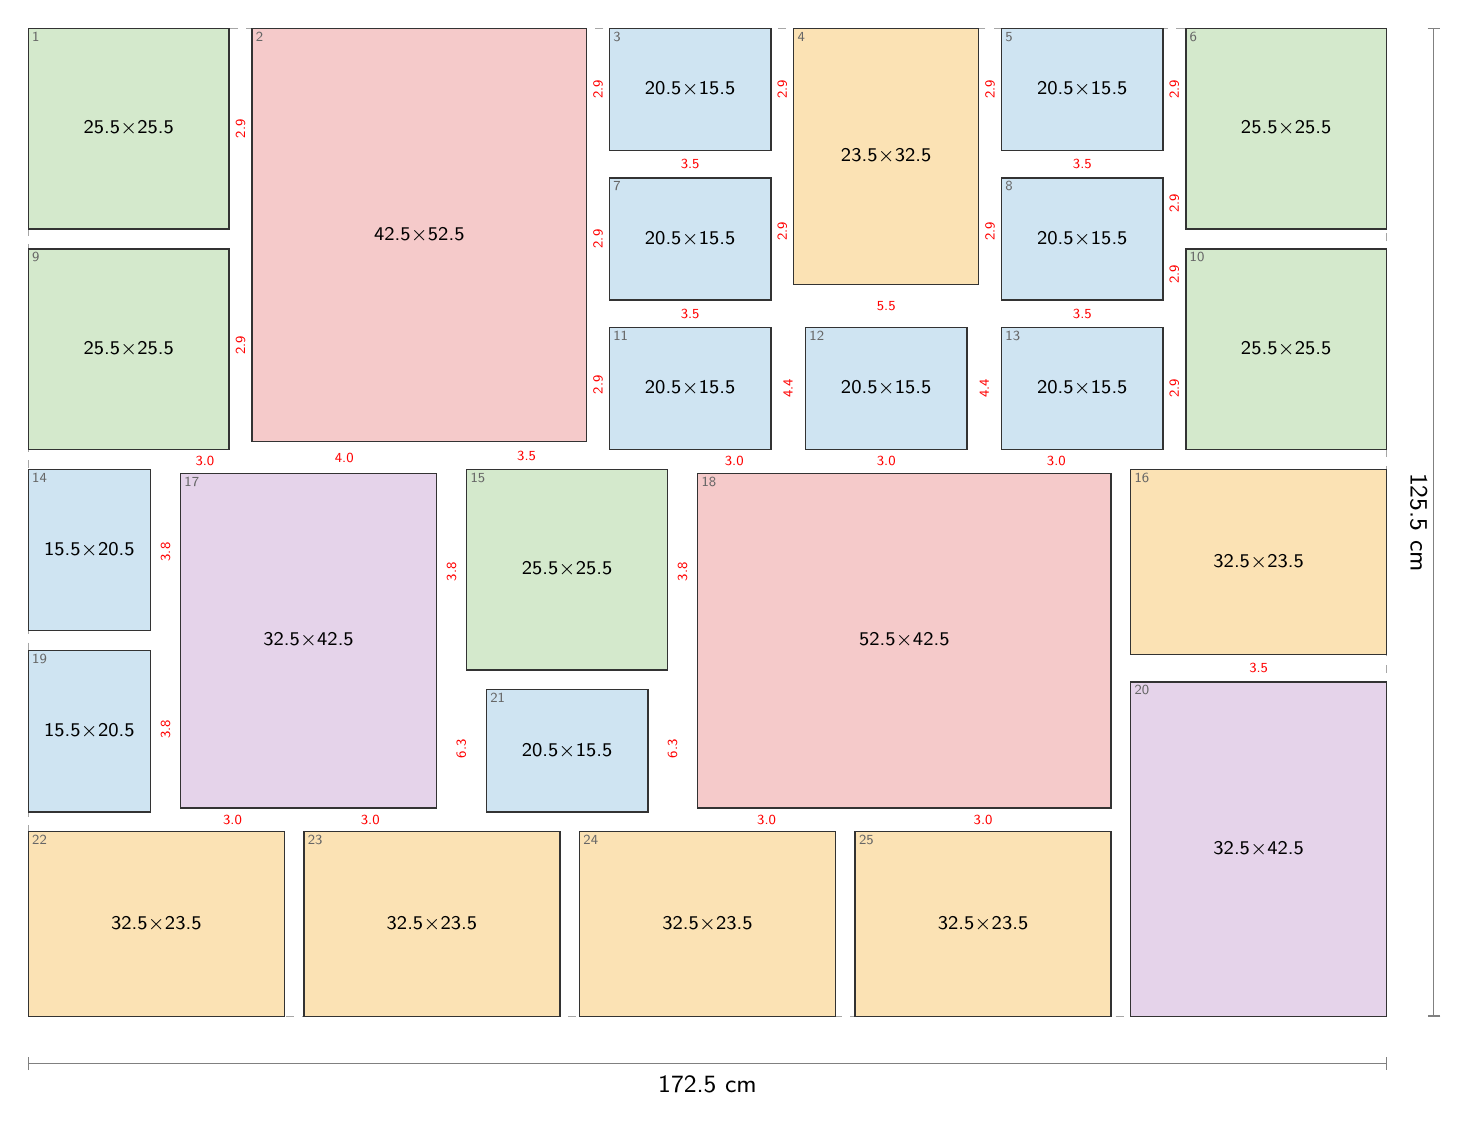
\begin{tikzpicture}[x=1mm, y=-1mm]
\draw[gray!70, dashed, line width=0.4pt] (0,0) rectangle (172.50,125.50);
\filldraw[fill=ft2, draw=black!80, line width=0.5pt] (0.00,0.00) rectangle (25.50,25.50);
\node[align=center, inner sep=0pt] at (12.75,12.75) {\scriptsize 25.5$\times$25.5};
\node[anchor=north west, inner sep=1.2pt, font=\tiny, text=black!60] at (0.00,0.00) {1};
\filldraw[fill=ft4, draw=black!80, line width=0.5pt] (28.40,0.00) rectangle (70.90,52.50);
\node[align=center, inner sep=0pt] at (49.65,26.25) {\scriptsize 42.5$\times$52.5};
\node[anchor=north west, inner sep=1.2pt, font=\tiny, text=black!60] at (28.40,0.00) {2};
\filldraw[fill=ft0, draw=black!80, line width=0.5pt] (73.80,0.00) rectangle (94.30,15.50);
\node[align=center, inner sep=0pt] at (84.05,7.75) {\scriptsize 20.5$\times$15.5};
\node[anchor=north west, inner sep=1.2pt, font=\tiny, text=black!60] at (73.80,0.00) {3};
\filldraw[fill=ft1, draw=black!80, line width=0.5pt] (97.20,0.00) rectangle (120.70,32.50);
\node[align=center, inner sep=0pt] at (108.95,16.25) {\scriptsize 23.5$\times$32.5};
\node[anchor=north west, inner sep=1.2pt, font=\tiny, text=black!60] at (97.20,0.00) {4};
\filldraw[fill=ft0, draw=black!80, line width=0.5pt] (123.60,0.00) rectangle (144.10,15.50);
\node[align=center, inner sep=0pt] at (133.85,7.75) {\scriptsize 20.5$\times$15.5};
\node[anchor=north west, inner sep=1.2pt, font=\tiny, text=black!60] at (123.60,0.00) {5};
\filldraw[fill=ft2, draw=black!80, line width=0.5pt] (147.00,0.00) rectangle (172.50,25.50);
\node[align=center, inner sep=0pt] at (159.75,12.75) {\scriptsize 25.5$\times$25.5};
\node[anchor=north west, inner sep=1.2pt, font=\tiny, text=black!60] at (147.00,0.00) {6};
\filldraw[fill=ft0, draw=black!80, line width=0.5pt] (73.80,19.00) rectangle (94.30,34.50);
\node[align=center, inner sep=0pt] at (84.05,26.75) {\scriptsize 20.5$\times$15.5};
\node[anchor=north west, inner sep=1.2pt, font=\tiny, text=black!60] at (73.80,19.00) {7};
\filldraw[fill=ft0, draw=black!80, line width=0.5pt] (123.60,19.00) rectangle (144.10,34.50);
\node[align=center, inner sep=0pt] at (133.85,26.75) {\scriptsize 20.5$\times$15.5};
\node[anchor=north west, inner sep=1.2pt, font=\tiny, text=black!60] at (123.60,19.00) {8};
\filldraw[fill=ft2, draw=black!80, line width=0.5pt] (0.00,28.00) rectangle (25.50,53.50);
\node[align=center, inner sep=0pt] at (12.75,40.75) {\scriptsize 25.5$\times$25.5};
\node[anchor=north west, inner sep=1.2pt, font=\tiny, text=black!60] at (0.00,28.00) {9};
\filldraw[fill=ft2, draw=black!80, line width=0.5pt] (147.00,28.00) rectangle (172.50,53.50);
\node[align=center, inner sep=0pt] at (159.75,40.75) {\scriptsize 25.5$\times$25.5};
\node[anchor=north west, inner sep=1.2pt, font=\tiny, text=black!60] at (147.00,28.00) {10};
\filldraw[fill=ft0, draw=black!80, line width=0.5pt] (73.80,38.00) rectangle (94.30,53.50);
\node[align=center, inner sep=0pt] at (84.05,45.75) {\scriptsize 20.5$\times$15.5};
\node[anchor=north west, inner sep=1.2pt, font=\tiny, text=black!60] at (73.80,38.00) {11};
\filldraw[fill=ft0, draw=black!80, line width=0.5pt] (98.70,38.00) rectangle (119.20,53.50);
\node[align=center, inner sep=0pt] at (108.95,45.75) {\scriptsize 20.5$\times$15.5};
\node[anchor=north west, inner sep=1.2pt, font=\tiny, text=black!60] at (98.70,38.00) {12};
\filldraw[fill=ft0, draw=black!80, line width=0.5pt] (123.60,38.00) rectangle (144.10,53.50);
\node[align=center, inner sep=0pt] at (133.85,45.75) {\scriptsize 20.5$\times$15.5};
\node[anchor=north west, inner sep=1.2pt, font=\tiny, text=black!60] at (123.60,38.00) {13};
\filldraw[fill=ft0, draw=black!80, line width=0.5pt] (0.00,56.00) rectangle (15.50,76.50);
\node[align=center, inner sep=0pt] at (7.75,66.25) {\scriptsize 15.5$\times$20.5};
\node[anchor=north west, inner sep=1.2pt, font=\tiny, text=black!60] at (0.00,56.00) {14};
\filldraw[fill=ft2, draw=black!80, line width=0.5pt] (55.67,56.00) rectangle (81.17,81.50);
\node[align=center, inner sep=0pt] at (68.42,68.75) {\scriptsize 25.5$\times$25.5};
\node[anchor=north west, inner sep=1.2pt, font=\tiny, text=black!60] at (55.67,56.00) {15};
\filldraw[fill=ft1, draw=black!80, line width=0.5pt] (140.00,56.00) rectangle (172.50,79.50);
\node[align=center, inner sep=0pt] at (156.25,67.75) {\scriptsize 32.5$\times$23.5};
\node[anchor=north west, inner sep=1.2pt, font=\tiny, text=black!60] at (140.00,56.00) {16};
\filldraw[fill=ft3, draw=black!80, line width=0.5pt] (19.33,56.50) rectangle (51.83,99.00);
\node[align=center, inner sep=0pt] at (35.58,77.75) {\scriptsize 32.5$\times$42.5};
\node[anchor=north west, inner sep=1.2pt, font=\tiny, text=black!60] at (19.33,56.50) {17};
\filldraw[fill=ft4, draw=black!80, line width=0.5pt] (85.00,56.50) rectangle (137.50,99.00);
\node[align=center, inner sep=0pt] at (111.25,77.75) {\scriptsize 52.5$\times$42.5};
\node[anchor=north west, inner sep=1.2pt, font=\tiny, text=black!60] at (85.00,56.50) {18};
\filldraw[fill=ft0, draw=black!80, line width=0.5pt] (0.00,79.00) rectangle (15.50,99.50);
\node[align=center, inner sep=0pt] at (7.75,89.25) {\scriptsize 15.5$\times$20.5};
\node[anchor=north west, inner sep=1.2pt, font=\tiny, text=black!60] at (0.00,79.00) {19};
\filldraw[fill=ft3, draw=black!80, line width=0.5pt] (140.00,83.00) rectangle (172.50,125.50);
\node[align=center, inner sep=0pt] at (156.25,104.25) {\scriptsize 32.5$\times$42.5};
\node[anchor=north west, inner sep=1.2pt, font=\tiny, text=black!60] at (140.00,83.00) {20};
\filldraw[fill=ft0, draw=black!80, line width=0.5pt] (58.17,84.00) rectangle (78.67,99.50);
\node[align=center, inner sep=0pt] at (68.42,91.75) {\scriptsize 20.5$\times$15.5};
\node[anchor=north west, inner sep=1.2pt, font=\tiny, text=black!60] at (58.17,84.00) {21};
\filldraw[fill=ft1, draw=black!80, line width=0.5pt] (0.00,102.00) rectangle (32.50,125.50);
\node[align=center, inner sep=0pt] at (16.25,113.75) {\scriptsize 32.5$\times$23.5};
\node[anchor=north west, inner sep=1.2pt, font=\tiny, text=black!60] at (0.00,102.00) {22};
\filldraw[fill=ft1, draw=black!80, line width=0.5pt] (35.00,102.00) rectangle (67.50,125.50);
\node[align=center, inner sep=0pt] at (51.25,113.75) {\scriptsize 32.5$\times$23.5};
\node[anchor=north west, inner sep=1.2pt, font=\tiny, text=black!60] at (35.00,102.00) {23};
\filldraw[fill=ft1, draw=black!80, line width=0.5pt] (70.00,102.00) rectangle (102.50,125.50);
\node[align=center, inner sep=0pt] at (86.25,113.75) {\scriptsize 32.5$\times$23.5};
\node[anchor=north west, inner sep=1.2pt, font=\tiny, text=black!60] at (70.00,102.00) {24};
\filldraw[fill=ft1, draw=black!80, line width=0.5pt] (105.00,102.00) rectangle (137.50,125.50);
\node[align=center, inner sep=0pt] at (121.25,113.75) {\scriptsize 32.5$\times$23.5};
\node[anchor=north west, inner sep=1.2pt, font=\tiny, text=black!60] at (105.00,102.00) {25};
\node[font=\tiny, text=red, fill=white, inner sep=0.3pt, rotate=90] at (26.95,12.75) {2.9};
\node[font=\tiny, text=red, fill=white, inner sep=0.3pt, rotate=90] at (72.35,7.75) {2.9};
\node[font=\tiny, text=red, fill=white, inner sep=0.3pt, rotate=90] at (72.35,26.75) {2.9};
\node[font=\tiny, text=red, fill=white, inner sep=0.3pt, rotate=90] at (72.35,45.25) {2.9};
\node[font=\tiny, text=red, fill=white, inner sep=0.3pt] at (63.28,54.25) {3.5};
\node[font=\tiny, text=red, fill=white, inner sep=0.3pt] at (40.12,54.50) {4.0};
\node[font=\tiny, text=red, fill=white, inner sep=0.3pt, rotate=90] at (95.75,7.75) {2.9};
\node[font=\tiny, text=red, fill=white, inner sep=0.3pt] at (84.05,17.25) {3.5};
\node[font=\tiny, text=red, fill=white, inner sep=0.3pt, rotate=90] at (122.15,7.75) {2.9};
\node[font=\tiny, text=red, fill=white, inner sep=0.3pt, rotate=90] at (122.15,25.75) {2.9};
\node[font=\tiny, text=red, fill=white, inner sep=0.3pt] at (108.95,35.25) {5.5};
\node[font=\tiny, text=red, fill=white, inner sep=0.3pt, rotate=90] at (145.55,7.75) {2.9};
\node[font=\tiny, text=red, fill=white, inner sep=0.3pt] at (133.85,17.25) {3.5};
\node[font=\tiny, text=red, fill=white, inner sep=0.3pt, rotate=90] at (95.75,25.75) {2.9};
\node[font=\tiny, text=red, fill=white, inner sep=0.3pt] at (84.05,36.25) {3.5};
\node[font=\tiny, text=red, fill=white, inner sep=0.3pt, rotate=90] at (145.55,22.25) {2.9};
\node[font=\tiny, text=red, fill=white, inner sep=0.3pt, rotate=90] at (145.55,31.25) {2.9};
\node[font=\tiny, text=red, fill=white, inner sep=0.3pt] at (133.85,36.25) {3.5};
\node[font=\tiny, text=red, fill=white, inner sep=0.3pt, rotate=90] at (26.95,40.25) {2.9};
\node[font=\tiny, text=red, fill=white, inner sep=0.3pt] at (22.42,55.00) {3.0};
\node[font=\tiny, text=red, fill=white, inner sep=0.3pt, rotate=90] at (96.50,45.75) {4.4};
\node[font=\tiny, text=red, fill=white, inner sep=0.3pt] at (89.65,55.00) {3.0};
\node[font=\tiny, text=red, fill=white, inner sep=0.3pt, rotate=90] at (121.40,45.75) {4.4};
\node[font=\tiny, text=red, fill=white, inner sep=0.3pt] at (108.95,55.00) {3.0};
\node[font=\tiny, text=red, fill=white, inner sep=0.3pt, rotate=90] at (145.55,45.75) {2.9};
\node[font=\tiny, text=red, fill=white, inner sep=0.3pt] at (130.55,55.00) {3.0};
\node[font=\tiny, text=red, fill=white, inner sep=0.3pt, rotate=90] at (17.42,66.50) {3.8};
\node[font=\tiny, text=red, fill=white, inner sep=0.3pt, rotate=90] at (83.08,69.00) {3.8};
\node[font=\tiny, text=red, fill=white, inner sep=0.3pt] at (156.25,81.25) {3.5};
\node[font=\tiny, text=red, fill=white, inner sep=0.3pt, rotate=90] at (53.75,69.00) {3.8};
\node[font=\tiny, text=red, fill=white, inner sep=0.3pt, rotate=90] at (55.00,91.50) {6.3};
\node[font=\tiny, text=red, fill=white, inner sep=0.3pt] at (25.92,100.50) {3.0};
\node[font=\tiny, text=red, fill=white, inner sep=0.3pt] at (43.42,100.50) {3.0};
\node[font=\tiny, text=red, fill=white, inner sep=0.3pt] at (93.75,100.50) {3.0};
\node[font=\tiny, text=red, fill=white, inner sep=0.3pt] at (121.25,100.50) {3.0};
\node[font=\tiny, text=red, fill=white, inner sep=0.3pt, rotate=90] at (17.42,89.00) {3.8};
\node[font=\tiny, text=red, fill=white, inner sep=0.3pt, rotate=90] at (81.83,91.50) {6.3};
\draw[Bar-Bar, gray] (0,131.50) -- (172.50,131.50) node[midway, below=1pt, font=\small, text=black] {172.5 cm};
\draw[Bar-Bar, gray] (178.50,0) -- (178.50,125.50) node[midway, right=1pt, font=\small, text=black, rotate=-90, anchor=north] {125.5 cm};
\end{tikzpicture}\\[4pt]
{\scriptsize Scale 1:10 (1 mm = 1 cm). Red numbers mark gaps that deviate from the nominal gap by more than 0.25 cm. Small grey numbers index the coordinate table.}
\end{minipage}\hfill
\begin{minipage}[t]{0.25\textwidth}\vspace{0pt}
\small
\begin{tabular}{@{}l l@{}}
\toprule
Outer size & 172.5 $\times$ 125.5 cm \\
Nominal gap & 2.5 cm \\
Actual gaps & 2.5 -- 6.3 cm \\
Max.\ deviation & 3.8 cm \\
Mean deviation & 0.69 cm \\
Border notches & none \\
Corners filled & 4 / 4 \\
Frames used & 25 of 28 \\
Large frames & {\scriptsize 2, not touching, min.\ dist.\ 80 cm} \\
Entropy & 0.78 \\
\quad {\scriptsize mix / variety} & {\scriptsize 0.82 / 0.77} \\
\quad {\scriptsize stagger / lines} & {\scriptsize 0.52 / 1.00 (1 through)} \\
\bottomrule
\end{tabular}

\vspace{8pt}
\scriptsize
\begin{tabular}{@{}c l l r r@{}}
\toprule
 & outer w $\times$ h (cm) &  & used & have \\
\midrule
\tikz[baseline=-0.6ex]\fill[ft0,draw=black!60] (0,0) rectangle (1.2ex,1.2ex); & 20.5$\times$15.5 & L & 8 & 9 \\
\tikz[baseline=-0.6ex]\fill[ft0,draw=black!60] (0,0) rectangle (1.2ex,1.2ex); & 15.5$\times$20.5 & P & 2 & 2 \\
\tikz[baseline=-0.6ex]\fill[ft3,draw=black!60] (0,0) rectangle (1.2ex,1.2ex); & 32.5$\times$42.5 & P & 2 & 2 \\
\tikz[baseline=-0.6ex]\fill[ft3,draw=black!60] (0,0) rectangle (1.2ex,1.2ex); & 42.5$\times$32.5 & L & 0 & 1 \\
\tikz[baseline=-0.6ex]\fill[ft1,draw=black!60] (0,0) rectangle (1.2ex,1.2ex); & 32.5$\times$23.5 & L & 5 & 5 \\
\tikz[baseline=-0.6ex]\fill[ft1,draw=black!60] (0,0) rectangle (1.2ex,1.2ex); & 23.5$\times$32.5 & P & 1 & 1 \\
\tikz[baseline=-0.6ex]\fill[ft2,draw=black!60] (0,0) rectangle (1.2ex,1.2ex); & 25.5$\times$25.5 &  & 5 & 5 \\
\tikz[baseline=-0.6ex]\fill[ft4,draw=black!60] (0,0) rectangle (1.2ex,1.2ex); & 42.5$\times$52.5 & P & 1 & 1 \\
\tikz[baseline=-0.6ex]\fill[ft4,draw=black!60] (0,0) rectangle (1.2ex,1.2ex); & 52.5$\times$42.5 & L & 1 & 2 \\
\bottomrule
\end{tabular}

\vspace{8pt}
{\bfseries Positions} (top-left corner, cm)\\[2pt]
\tiny
\begin{tabular}{@{}r l r r@{}}
\toprule
\# & frame w $\times$ h & x & y \\
\midrule
1 & 25.5 $\times$ 25.5 & 0.0 & 0.0 \\
2 & 42.5 $\times$ 52.5 & 28.4 & 0.0 \\
3 & 20.5 $\times$ 15.5 & 73.8 & 0.0 \\
4 & 23.5 $\times$ 32.5 & 97.2 & 0.0 \\
5 & 20.5 $\times$ 15.5 & 123.6 & 0.0 \\
6 & 25.5 $\times$ 25.5 & 147.0 & 0.0 \\
7 & 20.5 $\times$ 15.5 & 73.8 & 19.0 \\
8 & 20.5 $\times$ 15.5 & 123.6 & 19.0 \\
9 & 25.5 $\times$ 25.5 & 0.0 & 28.0 \\
10 & 25.5 $\times$ 25.5 & 147.0 & 28.0 \\
11 & 20.5 $\times$ 15.5 & 73.8 & 38.0 \\
12 & 20.5 $\times$ 15.5 & 98.7 & 38.0 \\
13 & 20.5 $\times$ 15.5 & 123.6 & 38.0 \\
14 & 15.5 $\times$ 20.5 & 0.0 & 56.0 \\
15 & 25.5 $\times$ 25.5 & 55.7 & 56.0 \\
16 & 32.5 $\times$ 23.5 & 140.0 & 56.0 \\
17 & 32.5 $\times$ 42.5 & 19.3 & 56.5 \\
18 & 52.5 $\times$ 42.5 & 85.0 & 56.5 \\
19 & 15.5 $\times$ 20.5 & 0.0 & 79.0 \\
20 & 32.5 $\times$ 42.5 & 140.0 & 83.0 \\
21 & 20.5 $\times$ 15.5 & 58.2 & 84.0 \\
22 & 32.5 $\times$ 23.5 & 0.0 & 102.0 \\
23 & 32.5 $\times$ 23.5 & 35.0 & 102.0 \\
24 & 32.5 $\times$ 23.5 & 70.0 & 102.0 \\
25 & 32.5 $\times$ 23.5 & 105.0 & 102.0 \\
\bottomrule
\end{tabular}
\end{minipage}
\clearpage

\begin{minipage}[t]{0.74\textwidth}\vspace{0pt}
{\LARGE\bfseries Layout 7}\hspace{1.5em}{\large 179.5 $\times$ 111.5 cm \quad gap 1.5 cm \quad 25 frames}\\[8pt]
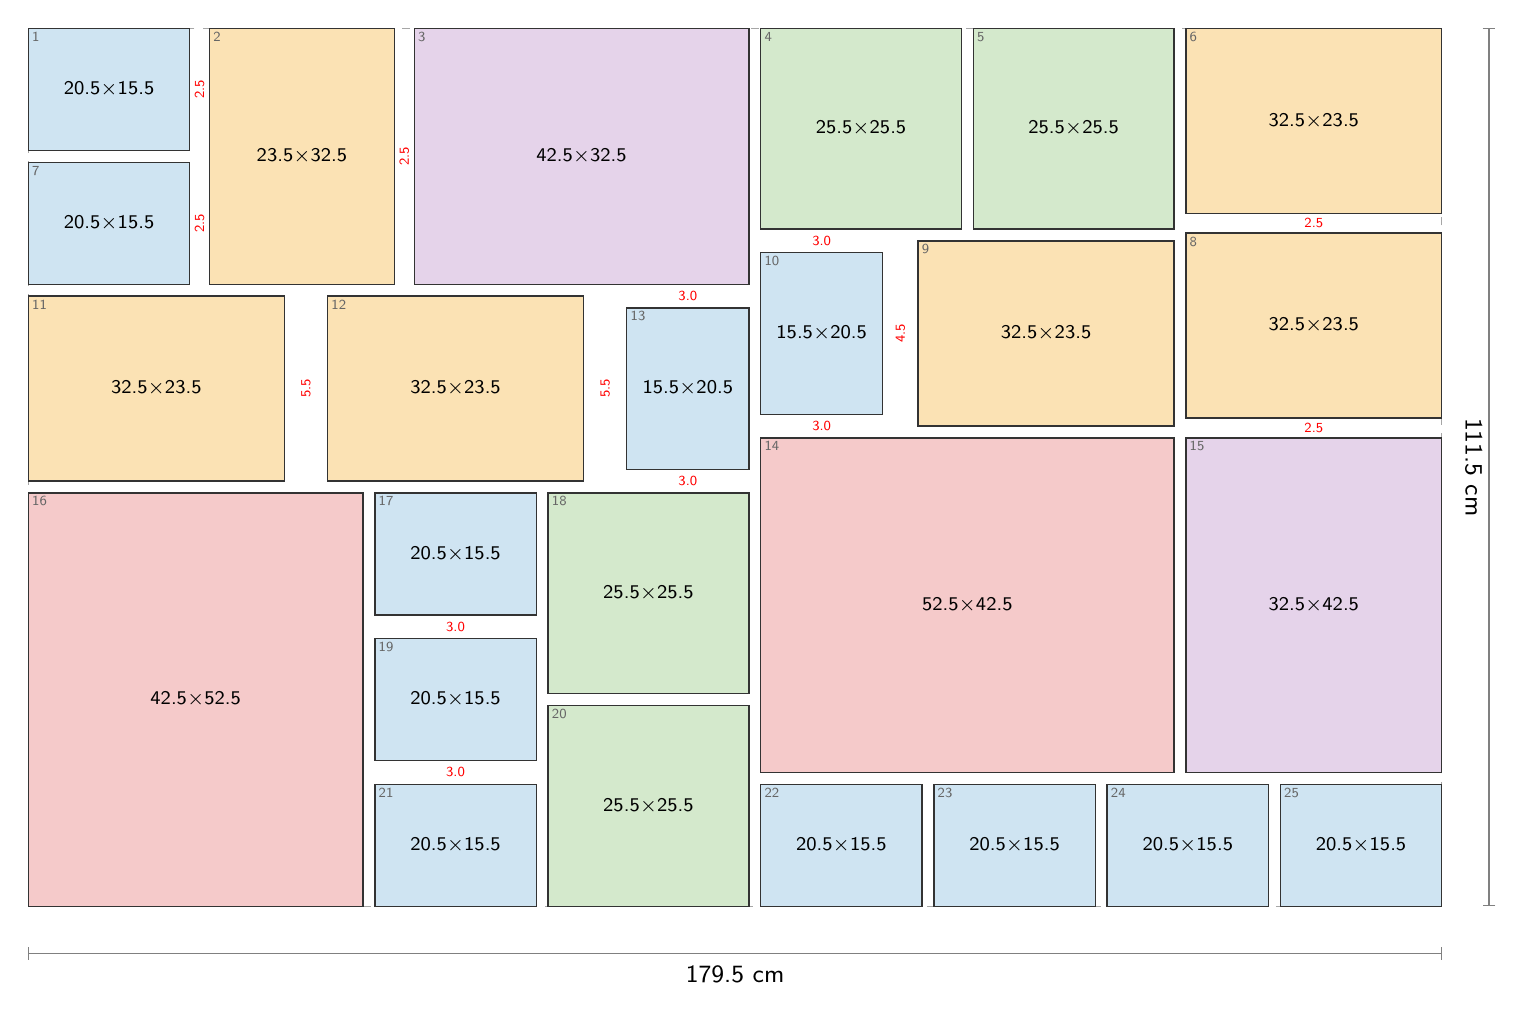
\begin{tikzpicture}[x=1mm, y=-1mm]
\draw[gray!70, dashed, line width=0.4pt] (0,0) rectangle (179.50,111.50);
\filldraw[fill=ft0, draw=black!80, line width=0.5pt] (0.00,0.00) rectangle (20.50,15.50);
\node[align=center, inner sep=0pt] at (10.25,7.75) {\scriptsize 20.5$\times$15.5};
\node[anchor=north west, inner sep=1.2pt, font=\tiny, text=black!60] at (0.00,0.00) {1};
\filldraw[fill=ft1, draw=black!80, line width=0.5pt] (23.00,0.00) rectangle (46.50,32.50);
\node[align=center, inner sep=0pt] at (34.75,16.25) {\scriptsize 23.5$\times$32.5};
\node[anchor=north west, inner sep=1.2pt, font=\tiny, text=black!60] at (23.00,0.00) {2};
\filldraw[fill=ft3, draw=black!80, line width=0.5pt] (49.00,0.00) rectangle (91.50,32.50);
\node[align=center, inner sep=0pt] at (70.25,16.25) {\scriptsize 42.5$\times$32.5};
\node[anchor=north west, inner sep=1.2pt, font=\tiny, text=black!60] at (49.00,0.00) {3};
\filldraw[fill=ft2, draw=black!80, line width=0.5pt] (93.00,0.00) rectangle (118.50,25.50);
\node[align=center, inner sep=0pt] at (105.75,12.75) {\scriptsize 25.5$\times$25.5};
\node[anchor=north west, inner sep=1.2pt, font=\tiny, text=black!60] at (93.00,0.00) {4};
\filldraw[fill=ft2, draw=black!80, line width=0.5pt] (120.00,0.00) rectangle (145.50,25.50);
\node[align=center, inner sep=0pt] at (132.75,12.75) {\scriptsize 25.5$\times$25.5};
\node[anchor=north west, inner sep=1.2pt, font=\tiny, text=black!60] at (120.00,0.00) {5};
\filldraw[fill=ft1, draw=black!80, line width=0.5pt] (147.00,0.00) rectangle (179.50,23.50);
\node[align=center, inner sep=0pt] at (163.25,11.75) {\scriptsize 32.5$\times$23.5};
\node[anchor=north west, inner sep=1.2pt, font=\tiny, text=black!60] at (147.00,0.00) {6};
\filldraw[fill=ft0, draw=black!80, line width=0.5pt] (0.00,17.00) rectangle (20.50,32.50);
\node[align=center, inner sep=0pt] at (10.25,24.75) {\scriptsize 20.5$\times$15.5};
\node[anchor=north west, inner sep=1.2pt, font=\tiny, text=black!60] at (0.00,17.00) {7};
\filldraw[fill=ft1, draw=black!80, line width=0.5pt] (147.00,26.00) rectangle (179.50,49.50);
\node[align=center, inner sep=0pt] at (163.25,37.75) {\scriptsize 32.5$\times$23.5};
\node[anchor=north west, inner sep=1.2pt, font=\tiny, text=black!60] at (147.00,26.00) {8};
\filldraw[fill=ft1, draw=black!80, line width=0.5pt] (113.00,27.00) rectangle (145.50,50.50);
\node[align=center, inner sep=0pt] at (129.25,38.75) {\scriptsize 32.5$\times$23.5};
\node[anchor=north west, inner sep=1.2pt, font=\tiny, text=black!60] at (113.00,27.00) {9};
\filldraw[fill=ft0, draw=black!80, line width=0.5pt] (93.00,28.50) rectangle (108.50,49.00);
\node[align=center, inner sep=0pt] at (100.75,38.75) {\scriptsize 15.5$\times$20.5};
\node[anchor=north west, inner sep=1.2pt, font=\tiny, text=black!60] at (93.00,28.50) {10};
\filldraw[fill=ft1, draw=black!80, line width=0.5pt] (0.00,34.00) rectangle (32.50,57.50);
\node[align=center, inner sep=0pt] at (16.25,45.75) {\scriptsize 32.5$\times$23.5};
\node[anchor=north west, inner sep=1.2pt, font=\tiny, text=black!60] at (0.00,34.00) {11};
\filldraw[fill=ft1, draw=black!80, line width=0.5pt] (38.00,34.00) rectangle (70.50,57.50);
\node[align=center, inner sep=0pt] at (54.25,45.75) {\scriptsize 32.5$\times$23.5};
\node[anchor=north west, inner sep=1.2pt, font=\tiny, text=black!60] at (38.00,34.00) {12};
\filldraw[fill=ft0, draw=black!80, line width=0.5pt] (76.00,35.50) rectangle (91.50,56.00);
\node[align=center, inner sep=0pt] at (83.75,45.75) {\scriptsize 15.5$\times$20.5};
\node[anchor=north west, inner sep=1.2pt, font=\tiny, text=black!60] at (76.00,35.50) {13};
\filldraw[fill=ft4, draw=black!80, line width=0.5pt] (93.00,52.00) rectangle (145.50,94.50);
\node[align=center, inner sep=0pt] at (119.25,73.25) {\scriptsize 52.5$\times$42.5};
\node[anchor=north west, inner sep=1.2pt, font=\tiny, text=black!60] at (93.00,52.00) {14};
\filldraw[fill=ft3, draw=black!80, line width=0.5pt] (147.00,52.00) rectangle (179.50,94.50);
\node[align=center, inner sep=0pt] at (163.25,73.25) {\scriptsize 32.5$\times$42.5};
\node[anchor=north west, inner sep=1.2pt, font=\tiny, text=black!60] at (147.00,52.00) {15};
\filldraw[fill=ft4, draw=black!80, line width=0.5pt] (0.00,59.00) rectangle (42.50,111.50);
\node[align=center, inner sep=0pt] at (21.25,85.25) {\scriptsize 42.5$\times$52.5};
\node[anchor=north west, inner sep=1.2pt, font=\tiny, text=black!60] at (0.00,59.00) {16};
\filldraw[fill=ft0, draw=black!80, line width=0.5pt] (44.00,59.00) rectangle (64.50,74.50);
\node[align=center, inner sep=0pt] at (54.25,66.75) {\scriptsize 20.5$\times$15.5};
\node[anchor=north west, inner sep=1.2pt, font=\tiny, text=black!60] at (44.00,59.00) {17};
\filldraw[fill=ft2, draw=black!80, line width=0.5pt] (66.00,59.00) rectangle (91.50,84.50);
\node[align=center, inner sep=0pt] at (78.75,71.75) {\scriptsize 25.5$\times$25.5};
\node[anchor=north west, inner sep=1.2pt, font=\tiny, text=black!60] at (66.00,59.00) {18};
\filldraw[fill=ft0, draw=black!80, line width=0.5pt] (44.00,77.50) rectangle (64.50,93.00);
\node[align=center, inner sep=0pt] at (54.25,85.25) {\scriptsize 20.5$\times$15.5};
\node[anchor=north west, inner sep=1.2pt, font=\tiny, text=black!60] at (44.00,77.50) {19};
\filldraw[fill=ft2, draw=black!80, line width=0.5pt] (66.00,86.00) rectangle (91.50,111.50);
\node[align=center, inner sep=0pt] at (78.75,98.75) {\scriptsize 25.5$\times$25.5};
\node[anchor=north west, inner sep=1.2pt, font=\tiny, text=black!60] at (66.00,86.00) {20};
\filldraw[fill=ft0, draw=black!80, line width=0.5pt] (44.00,96.00) rectangle (64.50,111.50);
\node[align=center, inner sep=0pt] at (54.25,103.75) {\scriptsize 20.5$\times$15.5};
\node[anchor=north west, inner sep=1.2pt, font=\tiny, text=black!60] at (44.00,96.00) {21};
\filldraw[fill=ft0, draw=black!80, line width=0.5pt] (93.00,96.00) rectangle (113.50,111.50);
\node[align=center, inner sep=0pt] at (103.25,103.75) {\scriptsize 20.5$\times$15.5};
\node[anchor=north west, inner sep=1.2pt, font=\tiny, text=black!60] at (93.00,96.00) {22};
\filldraw[fill=ft0, draw=black!80, line width=0.5pt] (115.00,96.00) rectangle (135.50,111.50);
\node[align=center, inner sep=0pt] at (125.25,103.75) {\scriptsize 20.5$\times$15.5};
\node[anchor=north west, inner sep=1.2pt, font=\tiny, text=black!60] at (115.00,96.00) {23};
\filldraw[fill=ft0, draw=black!80, line width=0.5pt] (137.00,96.00) rectangle (157.50,111.50);
\node[align=center, inner sep=0pt] at (147.25,103.75) {\scriptsize 20.5$\times$15.5};
\node[anchor=north west, inner sep=1.2pt, font=\tiny, text=black!60] at (137.00,96.00) {24};
\filldraw[fill=ft0, draw=black!80, line width=0.5pt] (159.00,96.00) rectangle (179.50,111.50);
\node[align=center, inner sep=0pt] at (169.25,103.75) {\scriptsize 20.5$\times$15.5};
\node[anchor=north west, inner sep=1.2pt, font=\tiny, text=black!60] at (159.00,96.00) {25};
\node[font=\tiny, text=red, fill=white, inner sep=0.3pt, rotate=90] at (21.75,7.75) {2.5};
\node[font=\tiny, text=red, fill=white, inner sep=0.3pt, rotate=90] at (47.75,16.25) {2.5};
\node[font=\tiny, text=red, fill=white, inner sep=0.3pt] at (83.75,34.00) {3.0};
\node[font=\tiny, text=red, fill=white, inner sep=0.3pt] at (100.75,27.00) {3.0};
\node[font=\tiny, text=red, fill=white, inner sep=0.3pt] at (163.25,24.75) {2.5};
\node[font=\tiny, text=red, fill=white, inner sep=0.3pt, rotate=90] at (21.75,24.75) {2.5};
\node[font=\tiny, text=red, fill=white, inner sep=0.3pt] at (163.25,50.75) {2.5};
\node[font=\tiny, text=red, fill=white, inner sep=0.3pt, rotate=90] at (110.75,38.75) {4.5};
\node[font=\tiny, text=red, fill=white, inner sep=0.3pt] at (100.75,50.50) {3.0};
\node[font=\tiny, text=red, fill=white, inner sep=0.3pt, rotate=90] at (35.25,45.75) {5.5};
\node[font=\tiny, text=red, fill=white, inner sep=0.3pt, rotate=90] at (73.25,45.75) {5.5};
\node[font=\tiny, text=red, fill=white, inner sep=0.3pt] at (83.75,57.50) {3.0};
\node[font=\tiny, text=red, fill=white, inner sep=0.3pt] at (54.25,76.00) {3.0};
\node[font=\tiny, text=red, fill=white, inner sep=0.3pt] at (54.25,94.50) {3.0};
\draw[Bar-Bar, gray] (0,117.50) -- (179.50,117.50) node[midway, below=1pt, font=\small, text=black] {179.5 cm};
\draw[Bar-Bar, gray] (185.50,0) -- (185.50,111.50) node[midway, right=1pt, font=\small, text=black, rotate=-90, anchor=north] {111.5 cm};
\end{tikzpicture}\\[4pt]
{\scriptsize Scale 1:10 (1 mm = 1 cm). Red numbers mark gaps that deviate from the nominal gap by more than 0.25 cm. Small grey numbers index the coordinate table.}
\end{minipage}\hfill
\begin{minipage}[t]{0.25\textwidth}\vspace{0pt}
\small
\begin{tabular}{@{}l l@{}}
\toprule
Outer size & 179.5 $\times$ 111.5 cm \\
Nominal gap & 1.5 cm \\
Actual gaps & 1.5 -- 5.5 cm \\
Max.\ deviation & 4.0 cm \\
Mean deviation & 0.51 cm \\
Border notches & none \\
Corners filled & 4 / 4 \\
Frames used & 25 of 28 \\
Large frames & {\scriptsize 2, not touching, min.\ dist.\ 99 cm} \\
Entropy & 0.79 \\
\quad {\scriptsize mix / variety} & {\scriptsize 0.83 / 0.78} \\
\quad {\scriptsize stagger / lines} & {\scriptsize 0.54 / 1.00 (1 through)} \\
\bottomrule
\end{tabular}

\vspace{8pt}
\scriptsize
\begin{tabular}{@{}c l l r r@{}}
\toprule
 & outer w $\times$ h (cm) &  & used & have \\
\midrule
\tikz[baseline=-0.6ex]\fill[ft0,draw=black!60] (0,0) rectangle (1.2ex,1.2ex); & 20.5$\times$15.5 & L & 9 & 9 \\
\tikz[baseline=-0.6ex]\fill[ft0,draw=black!60] (0,0) rectangle (1.2ex,1.2ex); & 15.5$\times$20.5 & P & 2 & 2 \\
\tikz[baseline=-0.6ex]\fill[ft3,draw=black!60] (0,0) rectangle (1.2ex,1.2ex); & 32.5$\times$42.5 & P & 1 & 2 \\
\tikz[baseline=-0.6ex]\fill[ft3,draw=black!60] (0,0) rectangle (1.2ex,1.2ex); & 42.5$\times$32.5 & L & 1 & 1 \\
\tikz[baseline=-0.6ex]\fill[ft1,draw=black!60] (0,0) rectangle (1.2ex,1.2ex); & 32.5$\times$23.5 & L & 5 & 5 \\
\tikz[baseline=-0.6ex]\fill[ft1,draw=black!60] (0,0) rectangle (1.2ex,1.2ex); & 23.5$\times$32.5 & P & 1 & 1 \\
\tikz[baseline=-0.6ex]\fill[ft2,draw=black!60] (0,0) rectangle (1.2ex,1.2ex); & 25.5$\times$25.5 &  & 4 & 5 \\
\tikz[baseline=-0.6ex]\fill[ft4,draw=black!60] (0,0) rectangle (1.2ex,1.2ex); & 42.5$\times$52.5 & P & 1 & 1 \\
\tikz[baseline=-0.6ex]\fill[ft4,draw=black!60] (0,0) rectangle (1.2ex,1.2ex); & 52.5$\times$42.5 & L & 1 & 2 \\
\bottomrule
\end{tabular}

\vspace{8pt}
{\bfseries Positions} (top-left corner, cm)\\[2pt]
\tiny
\begin{tabular}{@{}r l r r@{}}
\toprule
\# & frame w $\times$ h & x & y \\
\midrule
1 & 20.5 $\times$ 15.5 & 0.0 & 0.0 \\
2 & 23.5 $\times$ 32.5 & 23.0 & 0.0 \\
3 & 42.5 $\times$ 32.5 & 49.0 & 0.0 \\
4 & 25.5 $\times$ 25.5 & 93.0 & 0.0 \\
5 & 25.5 $\times$ 25.5 & 120.0 & 0.0 \\
6 & 32.5 $\times$ 23.5 & 147.0 & 0.0 \\
7 & 20.5 $\times$ 15.5 & 0.0 & 17.0 \\
8 & 32.5 $\times$ 23.5 & 147.0 & 26.0 \\
9 & 32.5 $\times$ 23.5 & 113.0 & 27.0 \\
10 & 15.5 $\times$ 20.5 & 93.0 & 28.5 \\
11 & 32.5 $\times$ 23.5 & 0.0 & 34.0 \\
12 & 32.5 $\times$ 23.5 & 38.0 & 34.0 \\
13 & 15.5 $\times$ 20.5 & 76.0 & 35.5 \\
14 & 52.5 $\times$ 42.5 & 93.0 & 52.0 \\
15 & 32.5 $\times$ 42.5 & 147.0 & 52.0 \\
16 & 42.5 $\times$ 52.5 & 0.0 & 59.0 \\
17 & 20.5 $\times$ 15.5 & 44.0 & 59.0 \\
18 & 25.5 $\times$ 25.5 & 66.0 & 59.0 \\
19 & 20.5 $\times$ 15.5 & 44.0 & 77.5 \\
20 & 25.5 $\times$ 25.5 & 66.0 & 86.0 \\
21 & 20.5 $\times$ 15.5 & 44.0 & 96.0 \\
22 & 20.5 $\times$ 15.5 & 93.0 & 96.0 \\
23 & 20.5 $\times$ 15.5 & 115.0 & 96.0 \\
24 & 20.5 $\times$ 15.5 & 137.0 & 96.0 \\
25 & 20.5 $\times$ 15.5 & 159.0 & 96.0 \\
\bottomrule
\end{tabular}
\end{minipage}
\clearpage

\begin{minipage}[t]{0.74\textwidth}\vspace{0pt}
{\LARGE\bfseries Layout 8}\hspace{1.5em}{\large 181.5 $\times$ 129.5 cm \quad gap 3.5 cm \quad 24 frames}\\[8pt]
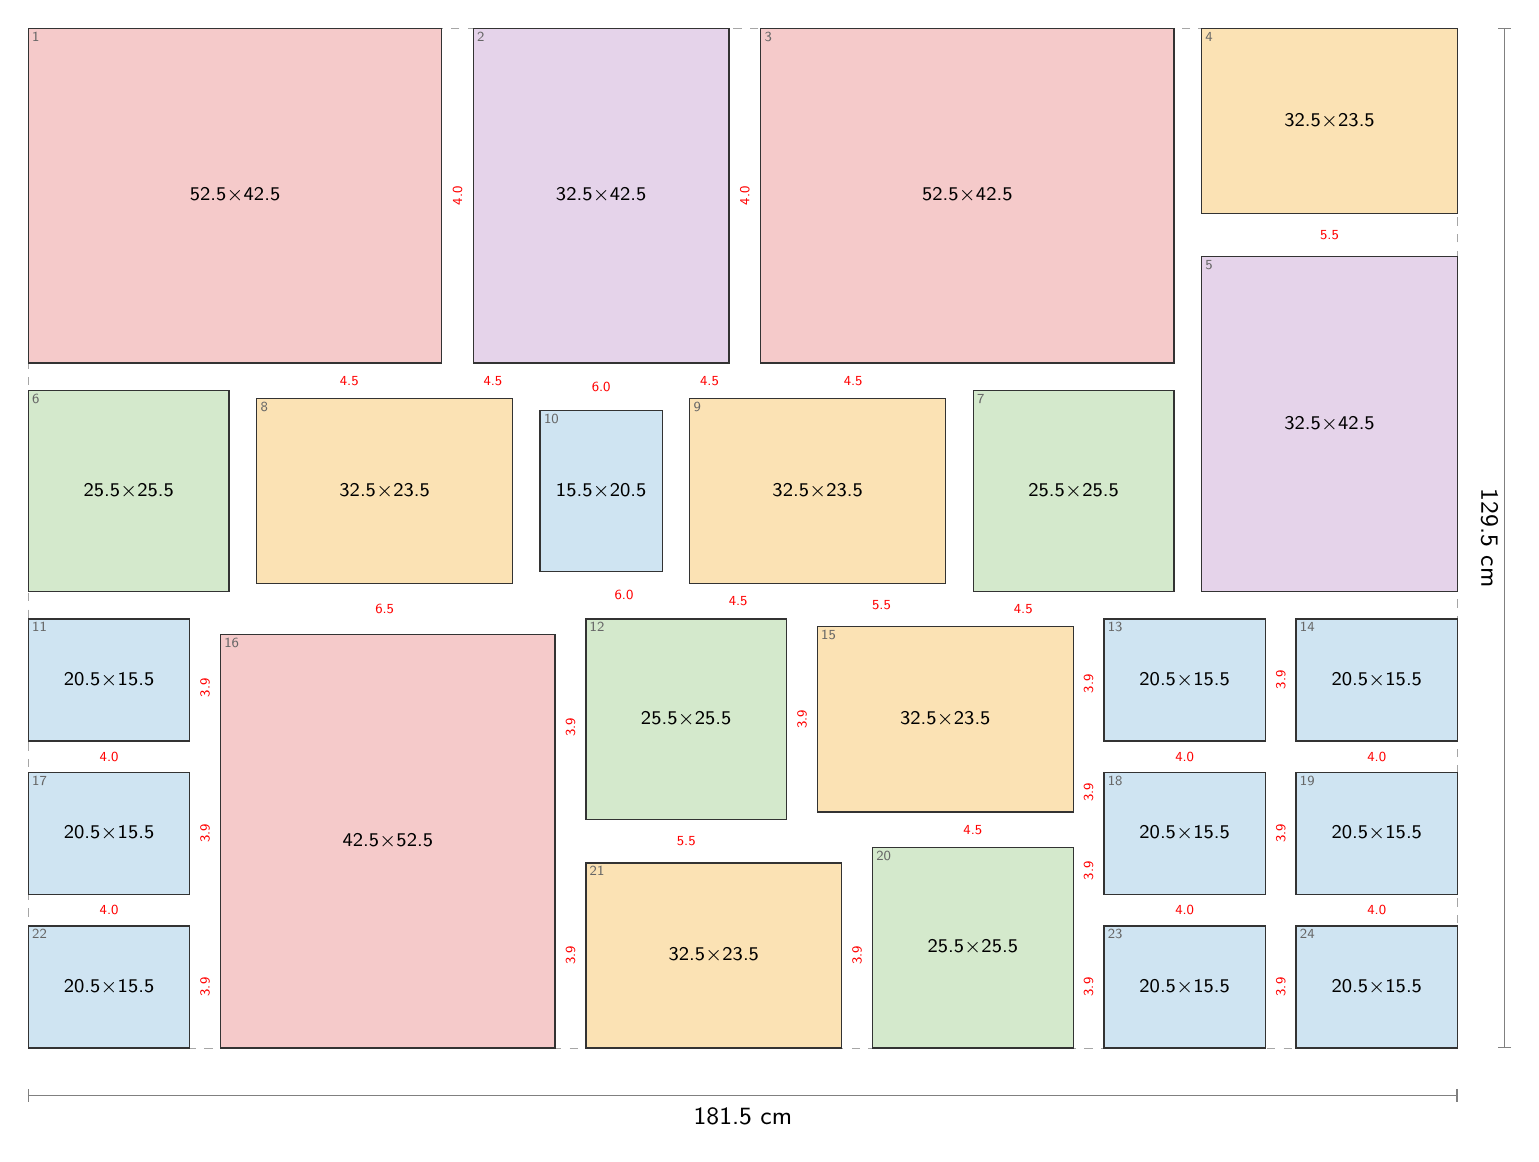
\begin{tikzpicture}[x=1mm, y=-1mm]
\draw[gray!70, dashed, line width=0.4pt] (0,0) rectangle (181.50,129.50);
\filldraw[fill=ft4, draw=black!80, line width=0.5pt] (0.00,0.00) rectangle (52.50,42.50);
\node[align=center, inner sep=0pt] at (26.25,21.25) {\scriptsize 52.5$\times$42.5};
\node[anchor=north west, inner sep=1.2pt, font=\tiny, text=black!60] at (0.00,0.00) {1};
\filldraw[fill=ft3, draw=black!80, line width=0.5pt] (56.50,0.00) rectangle (89.00,42.50);
\node[align=center, inner sep=0pt] at (72.75,21.25) {\scriptsize 32.5$\times$42.5};
\node[anchor=north west, inner sep=1.2pt, font=\tiny, text=black!60] at (56.50,0.00) {2};
\filldraw[fill=ft4, draw=black!80, line width=0.5pt] (93.00,0.00) rectangle (145.50,42.50);
\node[align=center, inner sep=0pt] at (119.25,21.25) {\scriptsize 52.5$\times$42.5};
\node[anchor=north west, inner sep=1.2pt, font=\tiny, text=black!60] at (93.00,0.00) {3};
\filldraw[fill=ft1, draw=black!80, line width=0.5pt] (149.00,0.00) rectangle (181.50,23.50);
\node[align=center, inner sep=0pt] at (165.25,11.75) {\scriptsize 32.5$\times$23.5};
\node[anchor=north west, inner sep=1.2pt, font=\tiny, text=black!60] at (149.00,0.00) {4};
\filldraw[fill=ft3, draw=black!80, line width=0.5pt] (149.00,29.00) rectangle (181.50,71.50);
\node[align=center, inner sep=0pt] at (165.25,50.25) {\scriptsize 32.5$\times$42.5};
\node[anchor=north west, inner sep=1.2pt, font=\tiny, text=black!60] at (149.00,29.00) {5};
\filldraw[fill=ft2, draw=black!80, line width=0.5pt] (0.00,46.00) rectangle (25.50,71.50);
\node[align=center, inner sep=0pt] at (12.75,58.75) {\scriptsize 25.5$\times$25.5};
\node[anchor=north west, inner sep=1.2pt, font=\tiny, text=black!60] at (0.00,46.00) {6};
\filldraw[fill=ft2, draw=black!80, line width=0.5pt] (120.00,46.00) rectangle (145.50,71.50);
\node[align=center, inner sep=0pt] at (132.75,58.75) {\scriptsize 25.5$\times$25.5};
\node[anchor=north west, inner sep=1.2pt, font=\tiny, text=black!60] at (120.00,46.00) {7};
\filldraw[fill=ft1, draw=black!80, line width=0.5pt] (29.00,47.00) rectangle (61.50,70.50);
\node[align=center, inner sep=0pt] at (45.25,58.75) {\scriptsize 32.5$\times$23.5};
\node[anchor=north west, inner sep=1.2pt, font=\tiny, text=black!60] at (29.00,47.00) {8};
\filldraw[fill=ft1, draw=black!80, line width=0.5pt] (84.00,47.00) rectangle (116.50,70.50);
\node[align=center, inner sep=0pt] at (100.25,58.75) {\scriptsize 32.5$\times$23.5};
\node[anchor=north west, inner sep=1.2pt, font=\tiny, text=black!60] at (84.00,47.00) {9};
\filldraw[fill=ft0, draw=black!80, line width=0.5pt] (65.00,48.50) rectangle (80.50,69.00);
\node[align=center, inner sep=0pt] at (72.75,58.75) {\scriptsize 15.5$\times$20.5};
\node[anchor=north west, inner sep=1.2pt, font=\tiny, text=black!60] at (65.00,48.50) {10};
\filldraw[fill=ft0, draw=black!80, line width=0.5pt] (0.00,75.00) rectangle (20.50,90.50);
\node[align=center, inner sep=0pt] at (10.25,82.75) {\scriptsize 20.5$\times$15.5};
\node[anchor=north west, inner sep=1.2pt, font=\tiny, text=black!60] at (0.00,75.00) {11};
\filldraw[fill=ft2, draw=black!80, line width=0.5pt] (70.80,75.00) rectangle (96.30,100.50);
\node[align=center, inner sep=0pt] at (83.55,87.75) {\scriptsize 25.5$\times$25.5};
\node[anchor=north west, inner sep=1.2pt, font=\tiny, text=black!60] at (70.80,75.00) {12};
\filldraw[fill=ft0, draw=black!80, line width=0.5pt] (136.60,75.00) rectangle (157.10,90.50);
\node[align=center, inner sep=0pt] at (146.85,82.75) {\scriptsize 20.5$\times$15.5};
\node[anchor=north west, inner sep=1.2pt, font=\tiny, text=black!60] at (136.60,75.00) {13};
\filldraw[fill=ft0, draw=black!80, line width=0.5pt] (161.00,75.00) rectangle (181.50,90.50);
\node[align=center, inner sep=0pt] at (171.25,82.75) {\scriptsize 20.5$\times$15.5};
\node[anchor=north west, inner sep=1.2pt, font=\tiny, text=black!60] at (161.00,75.00) {14};
\filldraw[fill=ft1, draw=black!80, line width=0.5pt] (100.20,76.00) rectangle (132.70,99.50);
\node[align=center, inner sep=0pt] at (116.45,87.75) {\scriptsize 32.5$\times$23.5};
\node[anchor=north west, inner sep=1.2pt, font=\tiny, text=black!60] at (100.20,76.00) {15};
\filldraw[fill=ft4, draw=black!80, line width=0.5pt] (24.40,77.00) rectangle (66.90,129.50);
\node[align=center, inner sep=0pt] at (45.65,103.25) {\scriptsize 42.5$\times$52.5};
\node[anchor=north west, inner sep=1.2pt, font=\tiny, text=black!60] at (24.40,77.00) {16};
\filldraw[fill=ft0, draw=black!80, line width=0.5pt] (0.00,94.50) rectangle (20.50,110.00);
\node[align=center, inner sep=0pt] at (10.25,102.25) {\scriptsize 20.5$\times$15.5};
\node[anchor=north west, inner sep=1.2pt, font=\tiny, text=black!60] at (0.00,94.50) {17};
\filldraw[fill=ft0, draw=black!80, line width=0.5pt] (136.60,94.50) rectangle (157.10,110.00);
\node[align=center, inner sep=0pt] at (146.85,102.25) {\scriptsize 20.5$\times$15.5};
\node[anchor=north west, inner sep=1.2pt, font=\tiny, text=black!60] at (136.60,94.50) {18};
\filldraw[fill=ft0, draw=black!80, line width=0.5pt] (161.00,94.50) rectangle (181.50,110.00);
\node[align=center, inner sep=0pt] at (171.25,102.25) {\scriptsize 20.5$\times$15.5};
\node[anchor=north west, inner sep=1.2pt, font=\tiny, text=black!60] at (161.00,94.50) {19};
\filldraw[fill=ft2, draw=black!80, line width=0.5pt] (107.20,104.00) rectangle (132.70,129.50);
\node[align=center, inner sep=0pt] at (119.95,116.75) {\scriptsize 25.5$\times$25.5};
\node[anchor=north west, inner sep=1.2pt, font=\tiny, text=black!60] at (107.20,104.00) {20};
\filldraw[fill=ft1, draw=black!80, line width=0.5pt] (70.80,106.00) rectangle (103.30,129.50);
\node[align=center, inner sep=0pt] at (87.05,117.75) {\scriptsize 32.5$\times$23.5};
\node[anchor=north west, inner sep=1.2pt, font=\tiny, text=black!60] at (70.80,106.00) {21};
\filldraw[fill=ft0, draw=black!80, line width=0.5pt] (0.00,114.00) rectangle (20.50,129.50);
\node[align=center, inner sep=0pt] at (10.25,121.75) {\scriptsize 20.5$\times$15.5};
\node[anchor=north west, inner sep=1.2pt, font=\tiny, text=black!60] at (0.00,114.00) {22};
\filldraw[fill=ft0, draw=black!80, line width=0.5pt] (136.60,114.00) rectangle (157.10,129.50);
\node[align=center, inner sep=0pt] at (146.85,121.75) {\scriptsize 20.5$\times$15.5};
\node[anchor=north west, inner sep=1.2pt, font=\tiny, text=black!60] at (136.60,114.00) {23};
\filldraw[fill=ft0, draw=black!80, line width=0.5pt] (161.00,114.00) rectangle (181.50,129.50);
\node[align=center, inner sep=0pt] at (171.25,121.75) {\scriptsize 20.5$\times$15.5};
\node[anchor=north west, inner sep=1.2pt, font=\tiny, text=black!60] at (161.00,114.00) {24};
\node[font=\tiny, text=red, fill=white, inner sep=0.3pt, rotate=90] at (54.50,21.25) {4.0};
\node[font=\tiny, text=red, fill=white, inner sep=0.3pt] at (40.75,44.75) {4.5};
\node[font=\tiny, text=red, fill=white, inner sep=0.3pt, rotate=90] at (91.00,21.25) {4.0};
\node[font=\tiny, text=red, fill=white, inner sep=0.3pt] at (59.00,44.75) {4.5};
\node[font=\tiny, text=red, fill=white, inner sep=0.3pt] at (86.50,44.75) {4.5};
\node[font=\tiny, text=red, fill=white, inner sep=0.3pt] at (72.75,45.50) {6.0};
\node[font=\tiny, text=red, fill=white, inner sep=0.3pt] at (104.75,44.75) {4.5};
\node[font=\tiny, text=red, fill=white, inner sep=0.3pt] at (165.25,26.25) {5.5};
\node[font=\tiny, text=red, fill=white, inner sep=0.3pt] at (126.35,73.75) {4.5};
\node[font=\tiny, text=red, fill=white, inner sep=0.3pt] at (45.25,73.75) {6.5};
\node[font=\tiny, text=red, fill=white, inner sep=0.3pt] at (90.15,72.75) {4.5};
\node[font=\tiny, text=red, fill=white, inner sep=0.3pt] at (108.35,73.25) {5.5};
\node[font=\tiny, text=red, fill=white, inner sep=0.3pt] at (75.65,72.00) {6.0};
\node[font=\tiny, text=red, fill=white, inner sep=0.3pt, rotate=90] at (22.45,83.75) {3.9};
\node[font=\tiny, text=red, fill=white, inner sep=0.3pt] at (10.25,92.50) {4.0};
\node[font=\tiny, text=red, fill=white, inner sep=0.3pt, rotate=90] at (98.25,87.75) {3.9};
\node[font=\tiny, text=red, fill=white, inner sep=0.3pt] at (83.55,103.25) {5.5};
\node[font=\tiny, text=red, fill=white, inner sep=0.3pt, rotate=90] at (159.05,82.75) {3.9};
\node[font=\tiny, text=red, fill=white, inner sep=0.3pt] at (146.85,92.50) {4.0};
\node[font=\tiny, text=red, fill=white, inner sep=0.3pt] at (171.25,92.50) {4.0};
\node[font=\tiny, text=red, fill=white, inner sep=0.3pt, rotate=90] at (134.65,83.25) {3.9};
\node[font=\tiny, text=red, fill=white, inner sep=0.3pt, rotate=90] at (134.65,97.00) {3.9};
\node[font=\tiny, text=red, fill=white, inner sep=0.3pt] at (119.95,101.75) {4.5};
\node[font=\tiny, text=red, fill=white, inner sep=0.3pt, rotate=90] at (68.85,88.75) {3.9};
\node[font=\tiny, text=red, fill=white, inner sep=0.3pt, rotate=90] at (68.85,117.75) {3.9};
\node[font=\tiny, text=red, fill=white, inner sep=0.3pt, rotate=90] at (22.45,102.25) {3.9};
\node[font=\tiny, text=red, fill=white, inner sep=0.3pt] at (10.25,112.00) {4.0};
\node[font=\tiny, text=red, fill=white, inner sep=0.3pt, rotate=90] at (159.05,102.25) {3.9};
\node[font=\tiny, text=red, fill=white, inner sep=0.3pt] at (146.85,112.00) {4.0};
\node[font=\tiny, text=red, fill=white, inner sep=0.3pt] at (171.25,112.00) {4.0};
\node[font=\tiny, text=red, fill=white, inner sep=0.3pt, rotate=90] at (134.65,107.00) {3.9};
\node[font=\tiny, text=red, fill=white, inner sep=0.3pt, rotate=90] at (134.65,121.75) {3.9};
\node[font=\tiny, text=red, fill=white, inner sep=0.3pt, rotate=90] at (105.25,117.75) {3.9};
\node[font=\tiny, text=red, fill=white, inner sep=0.3pt, rotate=90] at (22.45,121.75) {3.9};
\node[font=\tiny, text=red, fill=white, inner sep=0.3pt, rotate=90] at (159.05,121.75) {3.9};
\draw[Bar-Bar, gray] (0,135.50) -- (181.50,135.50) node[midway, below=1pt, font=\small, text=black] {181.5 cm};
\draw[Bar-Bar, gray] (187.50,0) -- (187.50,129.50) node[midway, right=1pt, font=\small, text=black, rotate=-90, anchor=north] {129.5 cm};
\end{tikzpicture}\\[4pt]
{\scriptsize Scale 1:10 (1 mm = 1 cm). Red numbers mark gaps that deviate from the nominal gap by more than 0.25 cm. Small grey numbers index the coordinate table.}
\end{minipage}\hfill
\begin{minipage}[t]{0.25\textwidth}\vspace{0pt}
\small
\begin{tabular}{@{}l l@{}}
\toprule
Outer size & 181.5 $\times$ 129.5 cm \\
Nominal gap & 3.5 cm \\
Actual gaps & 3.5 -- 6.5 cm \\
Max.\ deviation & 3.0 cm \\
Mean deviation & 0.64 cm \\
Border notches & right 6 cm \\
Corners filled & 4 / 4 \\
Frames used & 24 of 28 \\
Large frames & {\scriptsize 3, not touching, min.\ dist.\ 84 cm} \\
Entropy & 0.77 \\
\quad {\scriptsize mix / variety} & {\scriptsize 0.76 / 0.79} \\
\quad {\scriptsize stagger / lines} & {\scriptsize 0.52 / 1.00 (1 through)} \\
\bottomrule
\end{tabular}

\vspace{8pt}
\scriptsize
\begin{tabular}{@{}c l l r r@{}}
\toprule
 & outer w $\times$ h (cm) &  & used & have \\
\midrule
\tikz[baseline=-0.6ex]\fill[ft0,draw=black!60] (0,0) rectangle (1.2ex,1.2ex); & 20.5$\times$15.5 & L & 9 & 9 \\
\tikz[baseline=-0.6ex]\fill[ft0,draw=black!60] (0,0) rectangle (1.2ex,1.2ex); & 15.5$\times$20.5 & P & 1 & 2 \\
\tikz[baseline=-0.6ex]\fill[ft3,draw=black!60] (0,0) rectangle (1.2ex,1.2ex); & 32.5$\times$42.5 & P & 2 & 2 \\
\tikz[baseline=-0.6ex]\fill[ft3,draw=black!60] (0,0) rectangle (1.2ex,1.2ex); & 42.5$\times$32.5 & L & 0 & 1 \\
\tikz[baseline=-0.6ex]\fill[ft1,draw=black!60] (0,0) rectangle (1.2ex,1.2ex); & 32.5$\times$23.5 & L & 5 & 5 \\
\tikz[baseline=-0.6ex]\fill[ft1,draw=black!60] (0,0) rectangle (1.2ex,1.2ex); & 23.5$\times$32.5 & P & 0 & 1 \\
\tikz[baseline=-0.6ex]\fill[ft2,draw=black!60] (0,0) rectangle (1.2ex,1.2ex); & 25.5$\times$25.5 &  & 4 & 5 \\
\tikz[baseline=-0.6ex]\fill[ft4,draw=black!60] (0,0) rectangle (1.2ex,1.2ex); & 42.5$\times$52.5 & P & 1 & 1 \\
\tikz[baseline=-0.6ex]\fill[ft4,draw=black!60] (0,0) rectangle (1.2ex,1.2ex); & 52.5$\times$42.5 & L & 2 & 2 \\
\bottomrule
\end{tabular}

\vspace{8pt}
{\bfseries Positions} (top-left corner, cm)\\[2pt]
\tiny
\begin{tabular}{@{}r l r r@{}}
\toprule
\# & frame w $\times$ h & x & y \\
\midrule
1 & 52.5 $\times$ 42.5 & 0.0 & 0.0 \\
2 & 32.5 $\times$ 42.5 & 56.5 & 0.0 \\
3 & 52.5 $\times$ 42.5 & 93.0 & 0.0 \\
4 & 32.5 $\times$ 23.5 & 149.0 & 0.0 \\
5 & 32.5 $\times$ 42.5 & 149.0 & 29.0 \\
6 & 25.5 $\times$ 25.5 & 0.0 & 46.0 \\
7 & 25.5 $\times$ 25.5 & 120.0 & 46.0 \\
8 & 32.5 $\times$ 23.5 & 29.0 & 47.0 \\
9 & 32.5 $\times$ 23.5 & 84.0 & 47.0 \\
10 & 15.5 $\times$ 20.5 & 65.0 & 48.5 \\
11 & 20.5 $\times$ 15.5 & 0.0 & 75.0 \\
12 & 25.5 $\times$ 25.5 & 70.8 & 75.0 \\
13 & 20.5 $\times$ 15.5 & 136.6 & 75.0 \\
14 & 20.5 $\times$ 15.5 & 161.0 & 75.0 \\
15 & 32.5 $\times$ 23.5 & 100.2 & 76.0 \\
16 & 42.5 $\times$ 52.5 & 24.4 & 77.0 \\
17 & 20.5 $\times$ 15.5 & 0.0 & 94.5 \\
18 & 20.5 $\times$ 15.5 & 136.6 & 94.5 \\
19 & 20.5 $\times$ 15.5 & 161.0 & 94.5 \\
20 & 25.5 $\times$ 25.5 & 107.2 & 104.0 \\
21 & 32.5 $\times$ 23.5 & 70.8 & 106.0 \\
22 & 20.5 $\times$ 15.5 & 0.0 & 114.0 \\
23 & 20.5 $\times$ 15.5 & 136.6 & 114.0 \\
24 & 20.5 $\times$ 15.5 & 161.0 & 114.0 \\
\bottomrule
\end{tabular}
\end{minipage}
\clearpage

\begin{minipage}[t]{0.74\textwidth}\vspace{0pt}
{\LARGE\bfseries Layout 9}\hspace{1.5em}{\large 176.5 $\times$ 113.5 cm \quad gap 1.5 cm \quad 23 frames}\\[8pt]
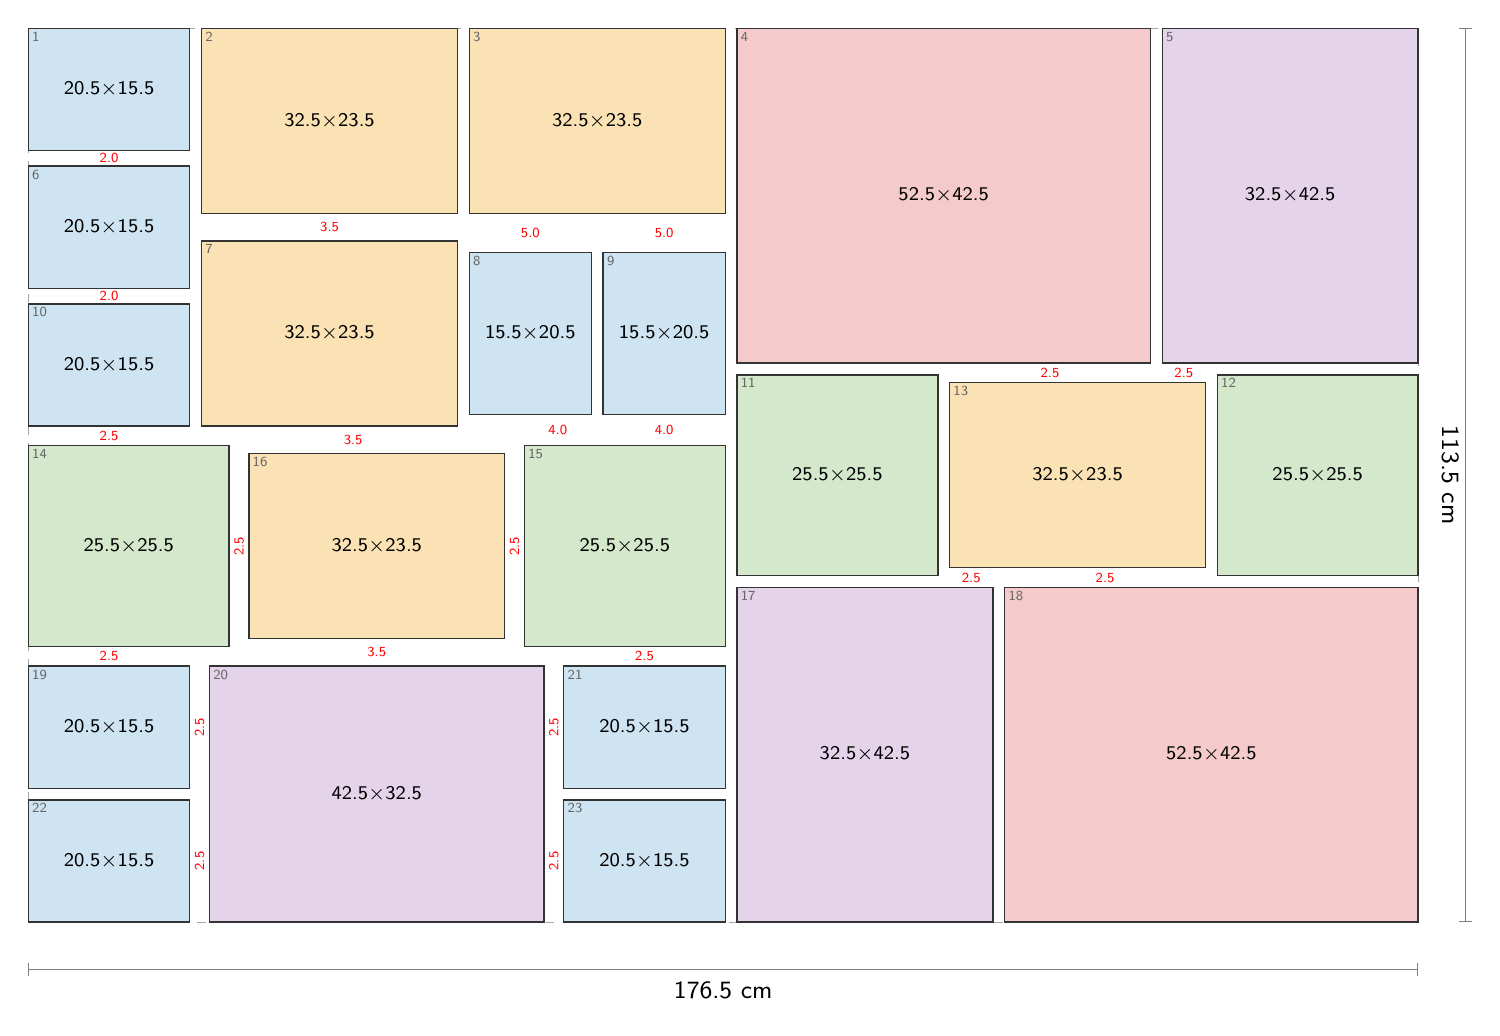
\begin{tikzpicture}[x=1mm, y=-1mm]
\draw[gray!70, dashed, line width=0.4pt] (0,0) rectangle (176.50,113.50);
\filldraw[fill=ft0, draw=black!80, line width=0.5pt] (0.00,0.00) rectangle (20.50,15.50);
\node[align=center, inner sep=0pt] at (10.25,7.75) {\scriptsize 20.5$\times$15.5};
\node[anchor=north west, inner sep=1.2pt, font=\tiny, text=black!60] at (0.00,0.00) {1};
\filldraw[fill=ft1, draw=black!80, line width=0.5pt] (22.00,0.00) rectangle (54.50,23.50);
\node[align=center, inner sep=0pt] at (38.25,11.75) {\scriptsize 32.5$\times$23.5};
\node[anchor=north west, inner sep=1.2pt, font=\tiny, text=black!60] at (22.00,0.00) {2};
\filldraw[fill=ft1, draw=black!80, line width=0.5pt] (56.00,0.00) rectangle (88.50,23.50);
\node[align=center, inner sep=0pt] at (72.25,11.75) {\scriptsize 32.5$\times$23.5};
\node[anchor=north west, inner sep=1.2pt, font=\tiny, text=black!60] at (56.00,0.00) {3};
\filldraw[fill=ft4, draw=black!80, line width=0.5pt] (90.00,0.00) rectangle (142.50,42.50);
\node[align=center, inner sep=0pt] at (116.25,21.25) {\scriptsize 52.5$\times$42.5};
\node[anchor=north west, inner sep=1.2pt, font=\tiny, text=black!60] at (90.00,0.00) {4};
\filldraw[fill=ft3, draw=black!80, line width=0.5pt] (144.00,0.00) rectangle (176.50,42.50);
\node[align=center, inner sep=0pt] at (160.25,21.25) {\scriptsize 32.5$\times$42.5};
\node[anchor=north west, inner sep=1.2pt, font=\tiny, text=black!60] at (144.00,0.00) {5};
\filldraw[fill=ft0, draw=black!80, line width=0.5pt] (0.00,17.50) rectangle (20.50,33.00);
\node[align=center, inner sep=0pt] at (10.25,25.25) {\scriptsize 20.5$\times$15.5};
\node[anchor=north west, inner sep=1.2pt, font=\tiny, text=black!60] at (0.00,17.50) {6};
\filldraw[fill=ft1, draw=black!80, line width=0.5pt] (22.00,27.00) rectangle (54.50,50.50);
\node[align=center, inner sep=0pt] at (38.25,38.75) {\scriptsize 32.5$\times$23.5};
\node[anchor=north west, inner sep=1.2pt, font=\tiny, text=black!60] at (22.00,27.00) {7};
\filldraw[fill=ft0, draw=black!80, line width=0.5pt] (56.00,28.50) rectangle (71.50,49.00);
\node[align=center, inner sep=0pt] at (63.75,38.75) {\scriptsize 15.5$\times$20.5};
\node[anchor=north west, inner sep=1.2pt, font=\tiny, text=black!60] at (56.00,28.50) {8};
\filldraw[fill=ft0, draw=black!80, line width=0.5pt] (73.00,28.50) rectangle (88.50,49.00);
\node[align=center, inner sep=0pt] at (80.75,38.75) {\scriptsize 15.5$\times$20.5};
\node[anchor=north west, inner sep=1.2pt, font=\tiny, text=black!60] at (73.00,28.50) {9};
\filldraw[fill=ft0, draw=black!80, line width=0.5pt] (0.00,35.00) rectangle (20.50,50.50);
\node[align=center, inner sep=0pt] at (10.25,42.75) {\scriptsize 20.5$\times$15.5};
\node[anchor=north west, inner sep=1.2pt, font=\tiny, text=black!60] at (0.00,35.00) {10};
\filldraw[fill=ft2, draw=black!80, line width=0.5pt] (90.00,44.00) rectangle (115.50,69.50);
\node[align=center, inner sep=0pt] at (102.75,56.75) {\scriptsize 25.5$\times$25.5};
\node[anchor=north west, inner sep=1.2pt, font=\tiny, text=black!60] at (90.00,44.00) {11};
\filldraw[fill=ft2, draw=black!80, line width=0.5pt] (151.00,44.00) rectangle (176.50,69.50);
\node[align=center, inner sep=0pt] at (163.75,56.75) {\scriptsize 25.5$\times$25.5};
\node[anchor=north west, inner sep=1.2pt, font=\tiny, text=black!60] at (151.00,44.00) {12};
\filldraw[fill=ft1, draw=black!80, line width=0.5pt] (117.00,45.00) rectangle (149.50,68.50);
\node[align=center, inner sep=0pt] at (133.25,56.75) {\scriptsize 32.5$\times$23.5};
\node[anchor=north west, inner sep=1.2pt, font=\tiny, text=black!60] at (117.00,45.00) {13};
\filldraw[fill=ft2, draw=black!80, line width=0.5pt] (0.00,53.00) rectangle (25.50,78.50);
\node[align=center, inner sep=0pt] at (12.75,65.75) {\scriptsize 25.5$\times$25.5};
\node[anchor=north west, inner sep=1.2pt, font=\tiny, text=black!60] at (0.00,53.00) {14};
\filldraw[fill=ft2, draw=black!80, line width=0.5pt] (63.00,53.00) rectangle (88.50,78.50);
\node[align=center, inner sep=0pt] at (75.75,65.75) {\scriptsize 25.5$\times$25.5};
\node[anchor=north west, inner sep=1.2pt, font=\tiny, text=black!60] at (63.00,53.00) {15};
\filldraw[fill=ft1, draw=black!80, line width=0.5pt] (28.00,54.00) rectangle (60.50,77.50);
\node[align=center, inner sep=0pt] at (44.25,65.75) {\scriptsize 32.5$\times$23.5};
\node[anchor=north west, inner sep=1.2pt, font=\tiny, text=black!60] at (28.00,54.00) {16};
\filldraw[fill=ft3, draw=black!80, line width=0.5pt] (90.00,71.00) rectangle (122.50,113.50);
\node[align=center, inner sep=0pt] at (106.25,92.25) {\scriptsize 32.5$\times$42.5};
\node[anchor=north west, inner sep=1.2pt, font=\tiny, text=black!60] at (90.00,71.00) {17};
\filldraw[fill=ft4, draw=black!80, line width=0.5pt] (124.00,71.00) rectangle (176.50,113.50);
\node[align=center, inner sep=0pt] at (150.25,92.25) {\scriptsize 52.5$\times$42.5};
\node[anchor=north west, inner sep=1.2pt, font=\tiny, text=black!60] at (124.00,71.00) {18};
\filldraw[fill=ft0, draw=black!80, line width=0.5pt] (0.00,81.00) rectangle (20.50,96.50);
\node[align=center, inner sep=0pt] at (10.25,88.75) {\scriptsize 20.5$\times$15.5};
\node[anchor=north west, inner sep=1.2pt, font=\tiny, text=black!60] at (0.00,81.00) {19};
\filldraw[fill=ft3, draw=black!80, line width=0.5pt] (23.00,81.00) rectangle (65.50,113.50);
\node[align=center, inner sep=0pt] at (44.25,97.25) {\scriptsize 42.5$\times$32.5};
\node[anchor=north west, inner sep=1.2pt, font=\tiny, text=black!60] at (23.00,81.00) {20};
\filldraw[fill=ft0, draw=black!80, line width=0.5pt] (68.00,81.00) rectangle (88.50,96.50);
\node[align=center, inner sep=0pt] at (78.25,88.75) {\scriptsize 20.5$\times$15.5};
\node[anchor=north west, inner sep=1.2pt, font=\tiny, text=black!60] at (68.00,81.00) {21};
\filldraw[fill=ft0, draw=black!80, line width=0.5pt] (0.00,98.00) rectangle (20.50,113.50);
\node[align=center, inner sep=0pt] at (10.25,105.75) {\scriptsize 20.5$\times$15.5};
\node[anchor=north west, inner sep=1.2pt, font=\tiny, text=black!60] at (0.00,98.00) {22};
\filldraw[fill=ft0, draw=black!80, line width=0.5pt] (68.00,98.00) rectangle (88.50,113.50);
\node[align=center, inner sep=0pt] at (78.25,105.75) {\scriptsize 20.5$\times$15.5};
\node[anchor=north west, inner sep=1.2pt, font=\tiny, text=black!60] at (68.00,98.00) {23};
\node[font=\tiny, text=red, fill=white, inner sep=0.3pt] at (10.25,16.50) {2.0};
\node[font=\tiny, text=red, fill=white, inner sep=0.3pt] at (38.25,25.25) {3.5};
\node[font=\tiny, text=red, fill=white, inner sep=0.3pt] at (63.75,26.00) {5.0};
\node[font=\tiny, text=red, fill=white, inner sep=0.3pt] at (80.75,26.00) {5.0};
\node[font=\tiny, text=red, fill=white, inner sep=0.3pt] at (129.75,43.75) {2.5};
\node[font=\tiny, text=red, fill=white, inner sep=0.3pt] at (146.75,43.75) {2.5};
\node[font=\tiny, text=red, fill=white, inner sep=0.3pt] at (10.25,34.00) {2.0};
\node[font=\tiny, text=red, fill=white, inner sep=0.3pt] at (41.25,52.25) {3.5};
\node[font=\tiny, text=red, fill=white, inner sep=0.3pt] at (67.25,51.00) {4.0};
\node[font=\tiny, text=red, fill=white, inner sep=0.3pt] at (80.75,51.00) {4.0};
\node[font=\tiny, text=red, fill=white, inner sep=0.3pt] at (10.25,51.75) {2.5};
\node[font=\tiny, text=red, fill=white, inner sep=0.3pt] at (119.75,69.75) {2.5};
\node[font=\tiny, text=red, fill=white, inner sep=0.3pt] at (136.75,69.75) {2.5};
\node[font=\tiny, text=red, fill=white, inner sep=0.3pt, rotate=90] at (26.75,65.75) {2.5};
\node[font=\tiny, text=red, fill=white, inner sep=0.3pt] at (10.25,79.75) {2.5};
\node[font=\tiny, text=red, fill=white, inner sep=0.3pt] at (78.25,79.75) {2.5};
\node[font=\tiny, text=red, fill=white, inner sep=0.3pt, rotate=90] at (61.75,65.75) {2.5};
\node[font=\tiny, text=red, fill=white, inner sep=0.3pt] at (44.25,79.25) {3.5};
\node[font=\tiny, text=red, fill=white, inner sep=0.3pt, rotate=90] at (21.75,88.75) {2.5};
\node[font=\tiny, text=red, fill=white, inner sep=0.3pt, rotate=90] at (66.75,88.75) {2.5};
\node[font=\tiny, text=red, fill=white, inner sep=0.3pt, rotate=90] at (66.75,105.75) {2.5};
\node[font=\tiny, text=red, fill=white, inner sep=0.3pt, rotate=90] at (21.75,105.75) {2.5};
\draw[Bar-Bar, gray] (0,119.50) -- (176.50,119.50) node[midway, below=1pt, font=\small, text=black] {176.5 cm};
\draw[Bar-Bar, gray] (182.50,0) -- (182.50,113.50) node[midway, right=1pt, font=\small, text=black, rotate=-90, anchor=north] {113.5 cm};
\end{tikzpicture}\\[4pt]
{\scriptsize Scale 1:10 (1 mm = 1 cm). Red numbers mark gaps that deviate from the nominal gap by more than 0.25 cm. Small grey numbers index the coordinate table.}
\end{minipage}\hfill
\begin{minipage}[t]{0.25\textwidth}\vspace{0pt}
\small
\begin{tabular}{@{}l l@{}}
\toprule
Outer size & 176.5 $\times$ 113.5 cm \\
Nominal gap & 1.5 cm \\
Actual gaps & 1.5 -- 5.0 cm \\
Max.\ deviation & 3.5 cm \\
Mean deviation & 0.70 cm \\
Border notches & none \\
Corners filled & 4 / 4 \\
Frames used & 23 of 28 \\
Large frames & {\scriptsize 2, not touching, min.\ dist.\ 79 cm} \\
Entropy & 0.79 \\
\quad {\scriptsize mix / variety} & {\scriptsize 0.81 / 0.82} \\
\quad {\scriptsize stagger / lines} & {\scriptsize 0.53 / 1.00 (1 through)} \\
\bottomrule
\end{tabular}

\vspace{8pt}
\scriptsize
\begin{tabular}{@{}c l l r r@{}}
\toprule
 & outer w $\times$ h (cm) &  & used & have \\
\midrule
\tikz[baseline=-0.6ex]\fill[ft0,draw=black!60] (0,0) rectangle (1.2ex,1.2ex); & 20.5$\times$15.5 & L & 7 & 9 \\
\tikz[baseline=-0.6ex]\fill[ft0,draw=black!60] (0,0) rectangle (1.2ex,1.2ex); & 15.5$\times$20.5 & P & 2 & 2 \\
\tikz[baseline=-0.6ex]\fill[ft3,draw=black!60] (0,0) rectangle (1.2ex,1.2ex); & 32.5$\times$42.5 & P & 2 & 2 \\
\tikz[baseline=-0.6ex]\fill[ft3,draw=black!60] (0,0) rectangle (1.2ex,1.2ex); & 42.5$\times$32.5 & L & 1 & 1 \\
\tikz[baseline=-0.6ex]\fill[ft1,draw=black!60] (0,0) rectangle (1.2ex,1.2ex); & 32.5$\times$23.5 & L & 5 & 5 \\
\tikz[baseline=-0.6ex]\fill[ft1,draw=black!60] (0,0) rectangle (1.2ex,1.2ex); & 23.5$\times$32.5 & P & 0 & 1 \\
\tikz[baseline=-0.6ex]\fill[ft2,draw=black!60] (0,0) rectangle (1.2ex,1.2ex); & 25.5$\times$25.5 &  & 4 & 5 \\
\tikz[baseline=-0.6ex]\fill[ft4,draw=black!60] (0,0) rectangle (1.2ex,1.2ex); & 42.5$\times$52.5 & P & 0 & 1 \\
\tikz[baseline=-0.6ex]\fill[ft4,draw=black!60] (0,0) rectangle (1.2ex,1.2ex); & 52.5$\times$42.5 & L & 2 & 2 \\
\bottomrule
\end{tabular}

\vspace{8pt}
{\bfseries Positions} (top-left corner, cm)\\[2pt]
\tiny
\begin{tabular}{@{}r l r r@{}}
\toprule
\# & frame w $\times$ h & x & y \\
\midrule
1 & 20.5 $\times$ 15.5 & 0.0 & 0.0 \\
2 & 32.5 $\times$ 23.5 & 22.0 & 0.0 \\
3 & 32.5 $\times$ 23.5 & 56.0 & 0.0 \\
4 & 52.5 $\times$ 42.5 & 90.0 & 0.0 \\
5 & 32.5 $\times$ 42.5 & 144.0 & 0.0 \\
6 & 20.5 $\times$ 15.5 & 0.0 & 17.5 \\
7 & 32.5 $\times$ 23.5 & 22.0 & 27.0 \\
8 & 15.5 $\times$ 20.5 & 56.0 & 28.5 \\
9 & 15.5 $\times$ 20.5 & 73.0 & 28.5 \\
10 & 20.5 $\times$ 15.5 & 0.0 & 35.0 \\
11 & 25.5 $\times$ 25.5 & 90.0 & 44.0 \\
12 & 25.5 $\times$ 25.5 & 151.0 & 44.0 \\
13 & 32.5 $\times$ 23.5 & 117.0 & 45.0 \\
14 & 25.5 $\times$ 25.5 & 0.0 & 53.0 \\
15 & 25.5 $\times$ 25.5 & 63.0 & 53.0 \\
16 & 32.5 $\times$ 23.5 & 28.0 & 54.0 \\
17 & 32.5 $\times$ 42.5 & 90.0 & 71.0 \\
18 & 52.5 $\times$ 42.5 & 124.0 & 71.0 \\
19 & 20.5 $\times$ 15.5 & 0.0 & 81.0 \\
20 & 42.5 $\times$ 32.5 & 23.0 & 81.0 \\
21 & 20.5 $\times$ 15.5 & 68.0 & 81.0 \\
22 & 20.5 $\times$ 15.5 & 0.0 & 98.0 \\
23 & 20.5 $\times$ 15.5 & 68.0 & 98.0 \\
\bottomrule
\end{tabular}
\end{minipage}
\clearpage

\begin{minipage}[t]{0.74\textwidth}\vspace{0pt}
{\LARGE\bfseries Layout 10}\hspace{1.5em}{\large 182.5 $\times$ 129.5 cm \quad gap 3.5 cm \quad 23 frames}\\[8pt]
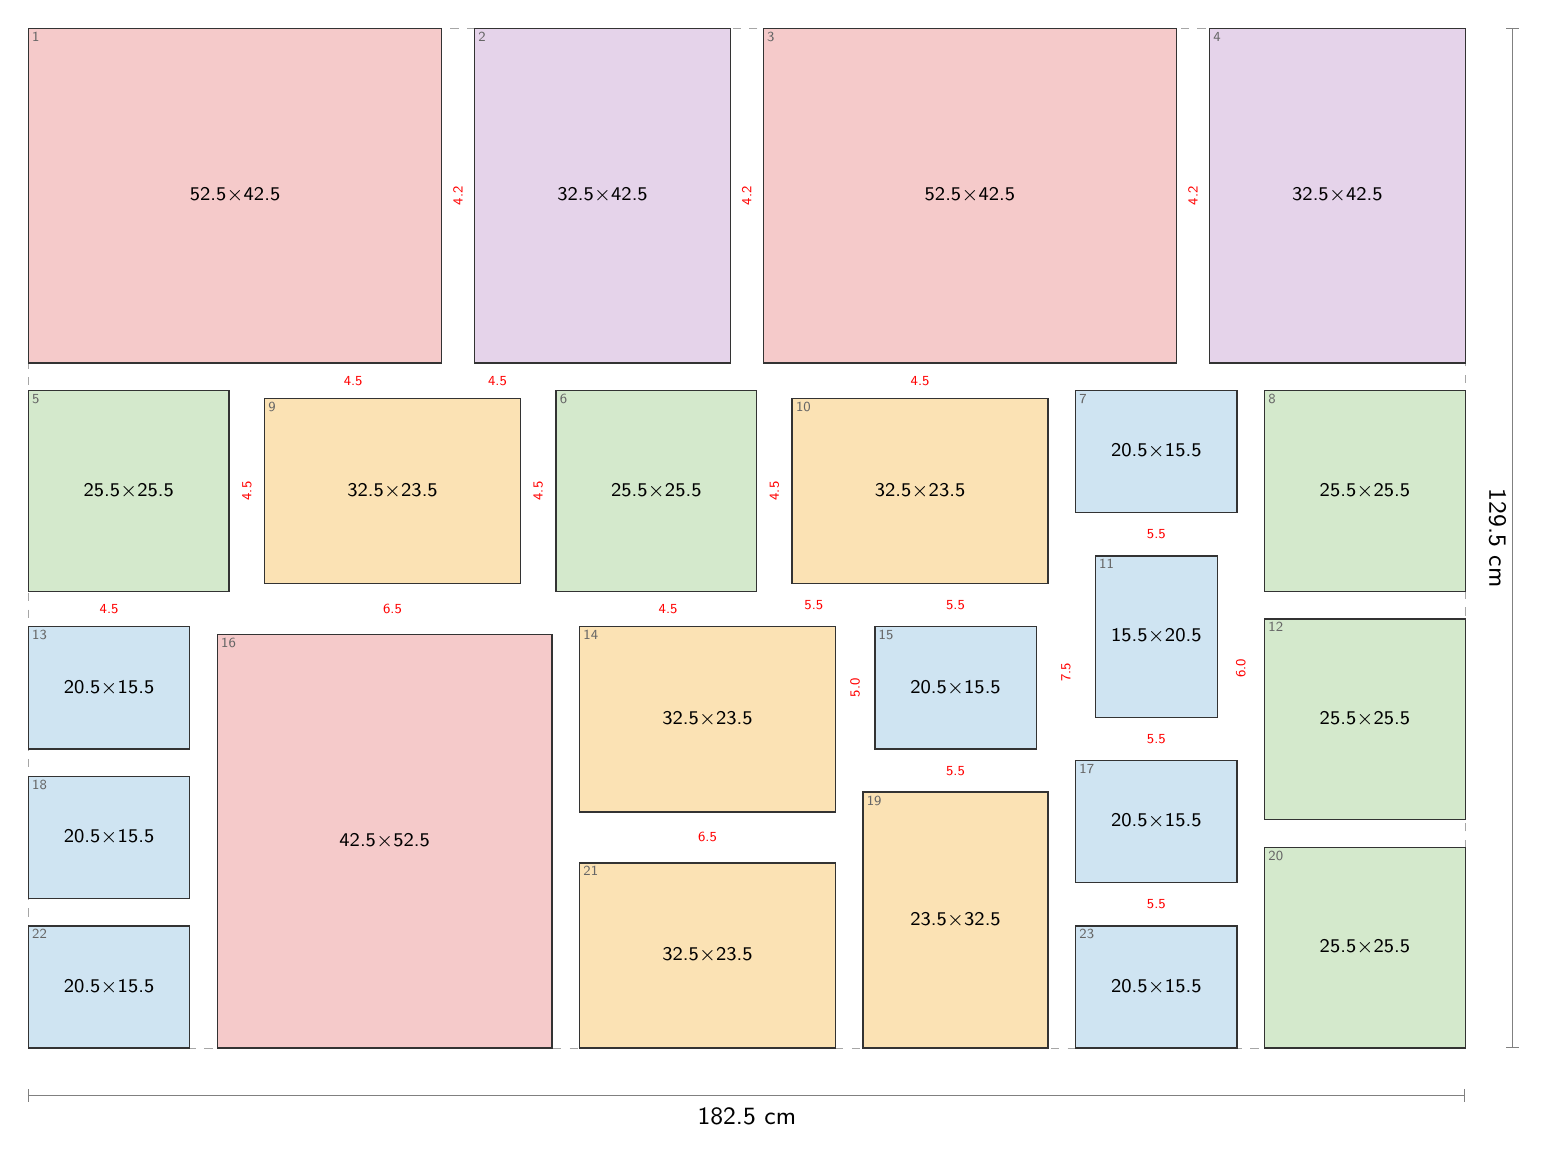
\begin{tikzpicture}[x=1mm, y=-1mm]
\draw[gray!70, dashed, line width=0.4pt] (0,0) rectangle (182.50,129.50);
\filldraw[fill=ft4, draw=black!80, line width=0.5pt] (0.00,0.00) rectangle (52.50,42.50);
\node[align=center, inner sep=0pt] at (26.25,21.25) {\scriptsize 52.5$\times$42.5};
\node[anchor=north west, inner sep=1.2pt, font=\tiny, text=black!60] at (0.00,0.00) {1};
\filldraw[fill=ft3, draw=black!80, line width=0.5pt] (56.67,0.00) rectangle (89.17,42.50);
\node[align=center, inner sep=0pt] at (72.92,21.25) {\scriptsize 32.5$\times$42.5};
\node[anchor=north west, inner sep=1.2pt, font=\tiny, text=black!60] at (56.67,0.00) {2};
\filldraw[fill=ft4, draw=black!80, line width=0.5pt] (93.33,0.00) rectangle (145.83,42.50);
\node[align=center, inner sep=0pt] at (119.58,21.25) {\scriptsize 52.5$\times$42.5};
\node[anchor=north west, inner sep=1.2pt, font=\tiny, text=black!60] at (93.33,0.00) {3};
\filldraw[fill=ft3, draw=black!80, line width=0.5pt] (150.00,0.00) rectangle (182.50,42.50);
\node[align=center, inner sep=0pt] at (166.25,21.25) {\scriptsize 32.5$\times$42.5};
\node[anchor=north west, inner sep=1.2pt, font=\tiny, text=black!60] at (150.00,0.00) {4};
\filldraw[fill=ft2, draw=black!80, line width=0.5pt] (0.00,46.00) rectangle (25.50,71.50);
\node[align=center, inner sep=0pt] at (12.75,58.75) {\scriptsize 25.5$\times$25.5};
\node[anchor=north west, inner sep=1.2pt, font=\tiny, text=black!60] at (0.00,46.00) {5};
\filldraw[fill=ft2, draw=black!80, line width=0.5pt] (67.00,46.00) rectangle (92.50,71.50);
\node[align=center, inner sep=0pt] at (79.75,58.75) {\scriptsize 25.5$\times$25.5};
\node[anchor=north west, inner sep=1.2pt, font=\tiny, text=black!60] at (67.00,46.00) {6};
\filldraw[fill=ft0, draw=black!80, line width=0.5pt] (133.00,46.00) rectangle (153.50,61.50);
\node[align=center, inner sep=0pt] at (143.25,53.75) {\scriptsize 20.5$\times$15.5};
\node[anchor=north west, inner sep=1.2pt, font=\tiny, text=black!60] at (133.00,46.00) {7};
\filldraw[fill=ft2, draw=black!80, line width=0.5pt] (157.00,46.00) rectangle (182.50,71.50);
\node[align=center, inner sep=0pt] at (169.75,58.75) {\scriptsize 25.5$\times$25.5};
\node[anchor=north west, inner sep=1.2pt, font=\tiny, text=black!60] at (157.00,46.00) {8};
\filldraw[fill=ft1, draw=black!80, line width=0.5pt] (30.00,47.00) rectangle (62.50,70.50);
\node[align=center, inner sep=0pt] at (46.25,58.75) {\scriptsize 32.5$\times$23.5};
\node[anchor=north west, inner sep=1.2pt, font=\tiny, text=black!60] at (30.00,47.00) {9};
\filldraw[fill=ft1, draw=black!80, line width=0.5pt] (97.00,47.00) rectangle (129.50,70.50);
\node[align=center, inner sep=0pt] at (113.25,58.75) {\scriptsize 32.5$\times$23.5};
\node[anchor=north west, inner sep=1.2pt, font=\tiny, text=black!60] at (97.00,47.00) {10};
\filldraw[fill=ft0, draw=black!80, line width=0.5pt] (135.50,67.00) rectangle (151.00,87.50);
\node[align=center, inner sep=0pt] at (143.25,77.25) {\scriptsize 15.5$\times$20.5};
\node[anchor=north west, inner sep=1.2pt, font=\tiny, text=black!60] at (135.50,67.00) {11};
\filldraw[fill=ft2, draw=black!80, line width=0.5pt] (157.00,75.00) rectangle (182.50,100.50);
\node[align=center, inner sep=0pt] at (169.75,87.75) {\scriptsize 25.5$\times$25.5};
\node[anchor=north west, inner sep=1.2pt, font=\tiny, text=black!60] at (157.00,75.00) {12};
\filldraw[fill=ft0, draw=black!80, line width=0.5pt] (0.00,76.00) rectangle (20.50,91.50);
\node[align=center, inner sep=0pt] at (10.25,83.75) {\scriptsize 20.5$\times$15.5};
\node[anchor=north west, inner sep=1.2pt, font=\tiny, text=black!60] at (0.00,76.00) {13};
\filldraw[fill=ft1, draw=black!80, line width=0.5pt] (70.00,76.00) rectangle (102.50,99.50);
\node[align=center, inner sep=0pt] at (86.25,87.75) {\scriptsize 32.5$\times$23.5};
\node[anchor=north west, inner sep=1.2pt, font=\tiny, text=black!60] at (70.00,76.00) {14};
\filldraw[fill=ft0, draw=black!80, line width=0.5pt] (107.50,76.00) rectangle (128.00,91.50);
\node[align=center, inner sep=0pt] at (117.75,83.75) {\scriptsize 20.5$\times$15.5};
\node[anchor=north west, inner sep=1.2pt, font=\tiny, text=black!60] at (107.50,76.00) {15};
\filldraw[fill=ft4, draw=black!80, line width=0.5pt] (24.00,77.00) rectangle (66.50,129.50);
\node[align=center, inner sep=0pt] at (45.25,103.25) {\scriptsize 42.5$\times$52.5};
\node[anchor=north west, inner sep=1.2pt, font=\tiny, text=black!60] at (24.00,77.00) {16};
\filldraw[fill=ft0, draw=black!80, line width=0.5pt] (133.00,93.00) rectangle (153.50,108.50);
\node[align=center, inner sep=0pt] at (143.25,100.75) {\scriptsize 20.5$\times$15.5};
\node[anchor=north west, inner sep=1.2pt, font=\tiny, text=black!60] at (133.00,93.00) {17};
\filldraw[fill=ft0, draw=black!80, line width=0.5pt] (0.00,95.00) rectangle (20.50,110.50);
\node[align=center, inner sep=0pt] at (10.25,102.75) {\scriptsize 20.5$\times$15.5};
\node[anchor=north west, inner sep=1.2pt, font=\tiny, text=black!60] at (0.00,95.00) {18};
\filldraw[fill=ft1, draw=black!80, line width=0.5pt] (106.00,97.00) rectangle (129.50,129.50);
\node[align=center, inner sep=0pt] at (117.75,113.25) {\scriptsize 23.5$\times$32.5};
\node[anchor=north west, inner sep=1.2pt, font=\tiny, text=black!60] at (106.00,97.00) {19};
\filldraw[fill=ft2, draw=black!80, line width=0.5pt] (157.00,104.00) rectangle (182.50,129.50);
\node[align=center, inner sep=0pt] at (169.75,116.75) {\scriptsize 25.5$\times$25.5};
\node[anchor=north west, inner sep=1.2pt, font=\tiny, text=black!60] at (157.00,104.00) {20};
\filldraw[fill=ft1, draw=black!80, line width=0.5pt] (70.00,106.00) rectangle (102.50,129.50);
\node[align=center, inner sep=0pt] at (86.25,117.75) {\scriptsize 32.5$\times$23.5};
\node[anchor=north west, inner sep=1.2pt, font=\tiny, text=black!60] at (70.00,106.00) {21};
\filldraw[fill=ft0, draw=black!80, line width=0.5pt] (0.00,114.00) rectangle (20.50,129.50);
\node[align=center, inner sep=0pt] at (10.25,121.75) {\scriptsize 20.5$\times$15.5};
\node[anchor=north west, inner sep=1.2pt, font=\tiny, text=black!60] at (0.00,114.00) {22};
\filldraw[fill=ft0, draw=black!80, line width=0.5pt] (133.00,114.00) rectangle (153.50,129.50);
\node[align=center, inner sep=0pt] at (143.25,121.75) {\scriptsize 20.5$\times$15.5};
\node[anchor=north west, inner sep=1.2pt, font=\tiny, text=black!60] at (133.00,114.00) {23};
\node[font=\tiny, text=red, fill=white, inner sep=0.3pt, rotate=90] at (54.58,21.25) {4.2};
\node[font=\tiny, text=red, fill=white, inner sep=0.3pt] at (41.25,44.75) {4.5};
\node[font=\tiny, text=red, fill=white, inner sep=0.3pt, rotate=90] at (91.25,21.25) {4.2};
\node[font=\tiny, text=red, fill=white, inner sep=0.3pt] at (59.58,44.75) {4.5};
\node[font=\tiny, text=red, fill=white, inner sep=0.3pt, rotate=90] at (147.92,21.25) {4.2};
\node[font=\tiny, text=red, fill=white, inner sep=0.3pt] at (113.25,44.75) {4.5};
\node[font=\tiny, text=red, fill=white, inner sep=0.3pt, rotate=90] at (27.75,58.75) {4.5};
\node[font=\tiny, text=red, fill=white, inner sep=0.3pt] at (10.25,73.75) {4.5};
\node[font=\tiny, text=red, fill=white, inner sep=0.3pt, rotate=90] at (94.75,58.75) {4.5};
\node[font=\tiny, text=red, fill=white, inner sep=0.3pt] at (81.25,73.75) {4.5};
\node[font=\tiny, text=red, fill=white, inner sep=0.3pt] at (143.25,64.25) {5.5};
\node[font=\tiny, text=red, fill=white, inner sep=0.3pt, rotate=90] at (64.75,58.75) {4.5};
\node[font=\tiny, text=red, fill=white, inner sep=0.3pt] at (46.25,73.75) {6.5};
\node[font=\tiny, text=red, fill=white, inner sep=0.3pt] at (99.75,73.25) {5.5};
\node[font=\tiny, text=red, fill=white, inner sep=0.3pt] at (117.75,73.25) {5.5};
\node[font=\tiny, text=red, fill=white, inner sep=0.3pt, rotate=90] at (154.00,81.25) {6.0};
\node[font=\tiny, text=red, fill=white, inner sep=0.3pt] at (143.25,90.25) {5.5};
\node[font=\tiny, text=red, fill=white, inner sep=0.3pt, rotate=90] at (105.00,83.75) {5.0};
\node[font=\tiny, text=red, fill=white, inner sep=0.3pt] at (86.25,102.75) {6.5};
\node[font=\tiny, text=red, fill=white, inner sep=0.3pt, rotate=90] at (131.75,81.75) {7.5};
\node[font=\tiny, text=red, fill=white, inner sep=0.3pt] at (117.75,94.25) {5.5};
\node[font=\tiny, text=red, fill=white, inner sep=0.3pt] at (143.25,111.25) {5.5};
\draw[Bar-Bar, gray] (0,135.50) -- (182.50,135.50) node[midway, below=1pt, font=\small, text=black] {182.5 cm};
\draw[Bar-Bar, gray] (188.50,0) -- (188.50,129.50) node[midway, right=1pt, font=\small, text=black, rotate=-90, anchor=north] {129.5 cm};
\end{tikzpicture}\\[4pt]
{\scriptsize Scale 1:10 (1 mm = 1 cm). Red numbers mark gaps that deviate from the nominal gap by more than 0.25 cm. Small grey numbers index the coordinate table.}
\end{minipage}\hfill
\begin{minipage}[t]{0.25\textwidth}\vspace{0pt}
\small
\begin{tabular}{@{}l l@{}}
\toprule
Outer size & 182.5 $\times$ 129.5 cm \\
Nominal gap & 3.5 cm \\
Actual gaps & 3.5 -- 7.5 cm \\
Max.\ deviation & 4.0 cm \\
Mean deviation & 0.86 cm \\
Border notches & none \\
Corners filled & 4 / 4 \\
Frames used & 23 of 28 \\
Large frames & {\scriptsize 3, not touching, min.\ dist.\ 84 cm} \\
Entropy & 0.82 \\
\quad {\scriptsize mix / variety} & {\scriptsize 0.83 / 0.87} \\
\quad {\scriptsize stagger / lines} & {\scriptsize 0.57 / 1.00 (1 through)} \\
\bottomrule
\end{tabular}

\vspace{8pt}
\scriptsize
\begin{tabular}{@{}c l l r r@{}}
\toprule
 & outer w $\times$ h (cm) &  & used & have \\
\midrule
\tikz[baseline=-0.6ex]\fill[ft0,draw=black!60] (0,0) rectangle (1.2ex,1.2ex); & 20.5$\times$15.5 & L & 7 & 9 \\
\tikz[baseline=-0.6ex]\fill[ft0,draw=black!60] (0,0) rectangle (1.2ex,1.2ex); & 15.5$\times$20.5 & P & 1 & 2 \\
\tikz[baseline=-0.6ex]\fill[ft3,draw=black!60] (0,0) rectangle (1.2ex,1.2ex); & 32.5$\times$42.5 & P & 2 & 2 \\
\tikz[baseline=-0.6ex]\fill[ft3,draw=black!60] (0,0) rectangle (1.2ex,1.2ex); & 42.5$\times$32.5 & L & 0 & 1 \\
\tikz[baseline=-0.6ex]\fill[ft1,draw=black!60] (0,0) rectangle (1.2ex,1.2ex); & 32.5$\times$23.5 & L & 4 & 5 \\
\tikz[baseline=-0.6ex]\fill[ft1,draw=black!60] (0,0) rectangle (1.2ex,1.2ex); & 23.5$\times$32.5 & P & 1 & 1 \\
\tikz[baseline=-0.6ex]\fill[ft2,draw=black!60] (0,0) rectangle (1.2ex,1.2ex); & 25.5$\times$25.5 &  & 5 & 5 \\
\tikz[baseline=-0.6ex]\fill[ft4,draw=black!60] (0,0) rectangle (1.2ex,1.2ex); & 42.5$\times$52.5 & P & 1 & 1 \\
\tikz[baseline=-0.6ex]\fill[ft4,draw=black!60] (0,0) rectangle (1.2ex,1.2ex); & 52.5$\times$42.5 & L & 2 & 2 \\
\bottomrule
\end{tabular}

\vspace{8pt}
{\bfseries Positions} (top-left corner, cm)\\[2pt]
\tiny
\begin{tabular}{@{}r l r r@{}}
\toprule
\# & frame w $\times$ h & x & y \\
\midrule
1 & 52.5 $\times$ 42.5 & 0.0 & 0.0 \\
2 & 32.5 $\times$ 42.5 & 56.7 & 0.0 \\
3 & 52.5 $\times$ 42.5 & 93.3 & 0.0 \\
4 & 32.5 $\times$ 42.5 & 150.0 & 0.0 \\
5 & 25.5 $\times$ 25.5 & 0.0 & 46.0 \\
6 & 25.5 $\times$ 25.5 & 67.0 & 46.0 \\
7 & 20.5 $\times$ 15.5 & 133.0 & 46.0 \\
8 & 25.5 $\times$ 25.5 & 157.0 & 46.0 \\
9 & 32.5 $\times$ 23.5 & 30.0 & 47.0 \\
10 & 32.5 $\times$ 23.5 & 97.0 & 47.0 \\
11 & 15.5 $\times$ 20.5 & 135.5 & 67.0 \\
12 & 25.5 $\times$ 25.5 & 157.0 & 75.0 \\
13 & 20.5 $\times$ 15.5 & 0.0 & 76.0 \\
14 & 32.5 $\times$ 23.5 & 70.0 & 76.0 \\
15 & 20.5 $\times$ 15.5 & 107.5 & 76.0 \\
16 & 42.5 $\times$ 52.5 & 24.0 & 77.0 \\
17 & 20.5 $\times$ 15.5 & 133.0 & 93.0 \\
18 & 20.5 $\times$ 15.5 & 0.0 & 95.0 \\
19 & 23.5 $\times$ 32.5 & 106.0 & 97.0 \\
20 & 25.5 $\times$ 25.5 & 157.0 & 104.0 \\
21 & 32.5 $\times$ 23.5 & 70.0 & 106.0 \\
22 & 20.5 $\times$ 15.5 & 0.0 & 114.0 \\
23 & 20.5 $\times$ 15.5 & 133.0 & 114.0 \\
\bottomrule
\end{tabular}
\end{minipage}
\clearpage

\begin{minipage}[t]{0.74\textwidth}\vspace{0pt}
{\LARGE\bfseries Layout 11}\hspace{1.5em}{\large 184.5 $\times$ 113.5 cm \quad gap 1.5 cm \quad 23 frames}\\[8pt]
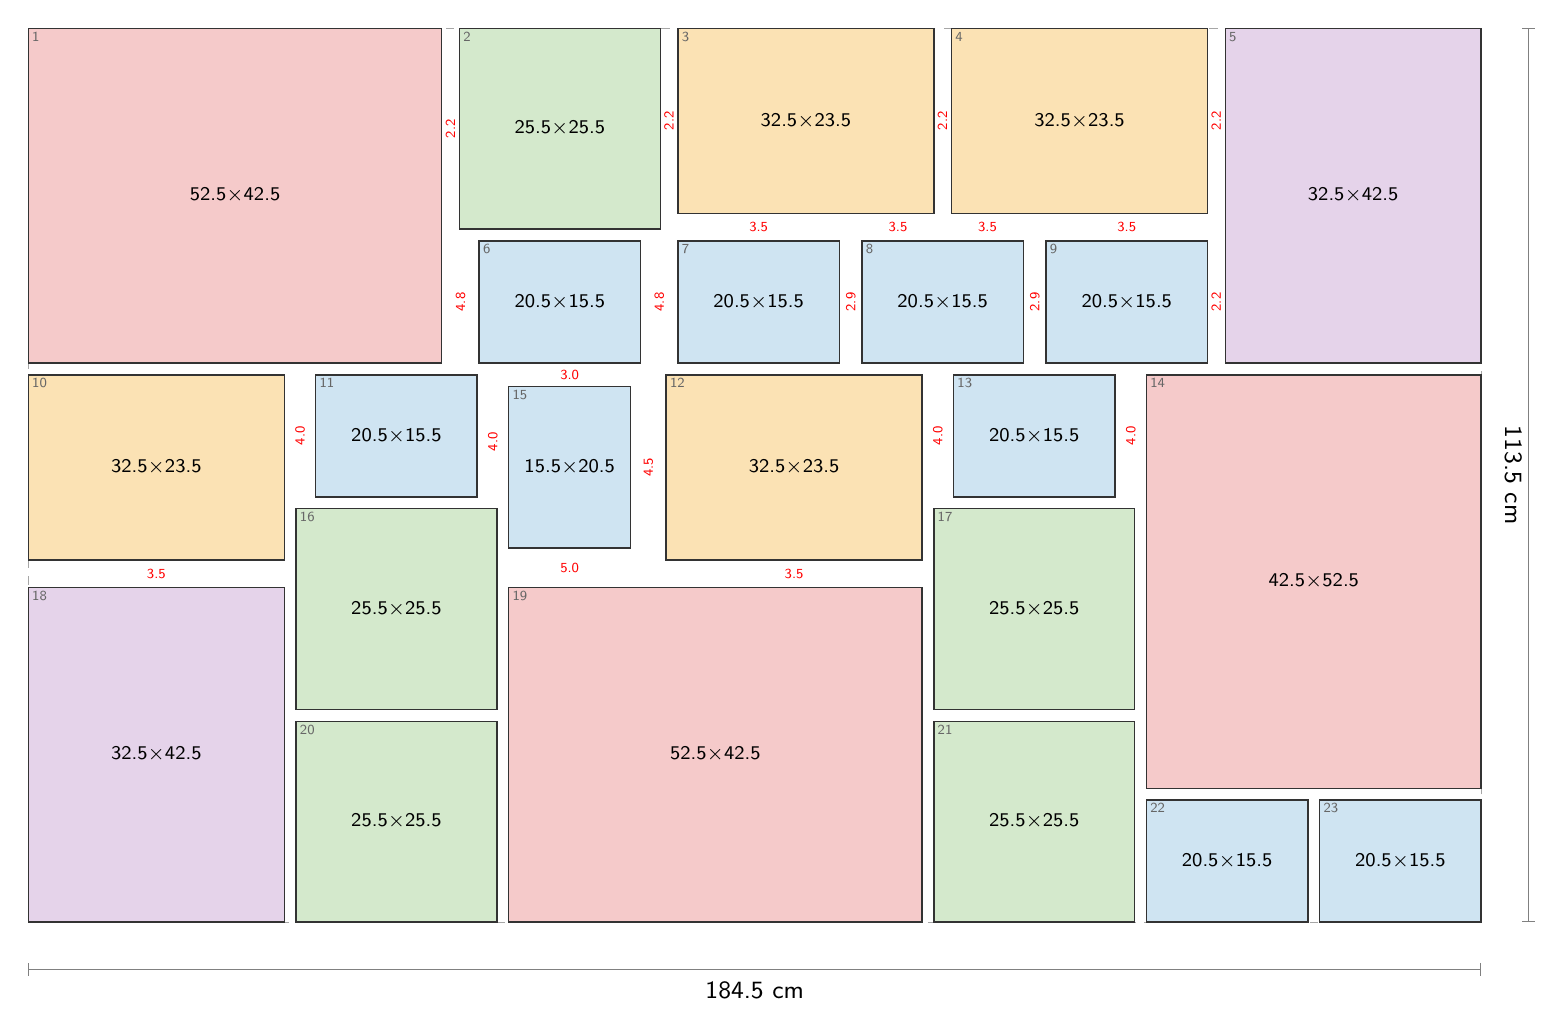
\begin{tikzpicture}[x=1mm, y=-1mm]
\draw[gray!70, dashed, line width=0.4pt] (0,0) rectangle (184.50,113.50);
\filldraw[fill=ft4, draw=black!80, line width=0.5pt] (0.00,0.00) rectangle (52.50,42.50);
\node[align=center, inner sep=0pt] at (26.25,21.25) {\scriptsize 52.5$\times$42.5};
\node[anchor=north west, inner sep=1.2pt, font=\tiny, text=black!60] at (0.00,0.00) {1};
\filldraw[fill=ft2, draw=black!80, line width=0.5pt] (54.75,0.00) rectangle (80.25,25.50);
\node[align=center, inner sep=0pt] at (67.50,12.75) {\scriptsize 25.5$\times$25.5};
\node[anchor=north west, inner sep=1.2pt, font=\tiny, text=black!60] at (54.75,0.00) {2};
\filldraw[fill=ft1, draw=black!80, line width=0.5pt] (82.50,0.00) rectangle (115.00,23.50);
\node[align=center, inner sep=0pt] at (98.75,11.75) {\scriptsize 32.5$\times$23.5};
\node[anchor=north west, inner sep=1.2pt, font=\tiny, text=black!60] at (82.50,0.00) {3};
\filldraw[fill=ft1, draw=black!80, line width=0.5pt] (117.25,0.00) rectangle (149.75,23.50);
\node[align=center, inner sep=0pt] at (133.50,11.75) {\scriptsize 32.5$\times$23.5};
\node[anchor=north west, inner sep=1.2pt, font=\tiny, text=black!60] at (117.25,0.00) {4};
\filldraw[fill=ft3, draw=black!80, line width=0.5pt] (152.00,0.00) rectangle (184.50,42.50);
\node[align=center, inner sep=0pt] at (168.25,21.25) {\scriptsize 32.5$\times$42.5};
\node[anchor=north west, inner sep=1.2pt, font=\tiny, text=black!60] at (152.00,0.00) {5};
\filldraw[fill=ft0, draw=black!80, line width=0.5pt] (57.25,27.00) rectangle (77.75,42.50);
\node[align=center, inner sep=0pt] at (67.50,34.75) {\scriptsize 20.5$\times$15.5};
\node[anchor=north west, inner sep=1.2pt, font=\tiny, text=black!60] at (57.25,27.00) {6};
\filldraw[fill=ft0, draw=black!80, line width=0.5pt] (82.50,27.00) rectangle (103.00,42.50);
\node[align=center, inner sep=0pt] at (92.75,34.75) {\scriptsize 20.5$\times$15.5};
\node[anchor=north west, inner sep=1.2pt, font=\tiny, text=black!60] at (82.50,27.00) {7};
\filldraw[fill=ft0, draw=black!80, line width=0.5pt] (105.88,27.00) rectangle (126.38,42.50);
\node[align=center, inner sep=0pt] at (116.12,34.75) {\scriptsize 20.5$\times$15.5};
\node[anchor=north west, inner sep=1.2pt, font=\tiny, text=black!60] at (105.88,27.00) {8};
\filldraw[fill=ft0, draw=black!80, line width=0.5pt] (129.25,27.00) rectangle (149.75,42.50);
\node[align=center, inner sep=0pt] at (139.50,34.75) {\scriptsize 20.5$\times$15.5};
\node[anchor=north west, inner sep=1.2pt, font=\tiny, text=black!60] at (129.25,27.00) {9};
\filldraw[fill=ft1, draw=black!80, line width=0.5pt] (0.00,44.00) rectangle (32.50,67.50);
\node[align=center, inner sep=0pt] at (16.25,55.75) {\scriptsize 32.5$\times$23.5};
\node[anchor=north west, inner sep=1.2pt, font=\tiny, text=black!60] at (0.00,44.00) {10};
\filldraw[fill=ft0, draw=black!80, line width=0.5pt] (36.50,44.00) rectangle (57.00,59.50);
\node[align=center, inner sep=0pt] at (46.75,51.75) {\scriptsize 20.5$\times$15.5};
\node[anchor=north west, inner sep=1.2pt, font=\tiny, text=black!60] at (36.50,44.00) {11};
\filldraw[fill=ft1, draw=black!80, line width=0.5pt] (81.00,44.00) rectangle (113.50,67.50);
\node[align=center, inner sep=0pt] at (97.25,55.75) {\scriptsize 32.5$\times$23.5};
\node[anchor=north west, inner sep=1.2pt, font=\tiny, text=black!60] at (81.00,44.00) {12};
\filldraw[fill=ft0, draw=black!80, line width=0.5pt] (117.50,44.00) rectangle (138.00,59.50);
\node[align=center, inner sep=0pt] at (127.75,51.75) {\scriptsize 20.5$\times$15.5};
\node[anchor=north west, inner sep=1.2pt, font=\tiny, text=black!60] at (117.50,44.00) {13};
\filldraw[fill=ft4, draw=black!80, line width=0.5pt] (142.00,44.00) rectangle (184.50,96.50);
\node[align=center, inner sep=0pt] at (163.25,70.25) {\scriptsize 42.5$\times$52.5};
\node[anchor=north west, inner sep=1.2pt, font=\tiny, text=black!60] at (142.00,44.00) {14};
\filldraw[fill=ft0, draw=black!80, line width=0.5pt] (61.00,45.50) rectangle (76.50,66.00);
\node[align=center, inner sep=0pt] at (68.75,55.75) {\scriptsize 15.5$\times$20.5};
\node[anchor=north west, inner sep=1.2pt, font=\tiny, text=black!60] at (61.00,45.50) {15};
\filldraw[fill=ft2, draw=black!80, line width=0.5pt] (34.00,61.00) rectangle (59.50,86.50);
\node[align=center, inner sep=0pt] at (46.75,73.75) {\scriptsize 25.5$\times$25.5};
\node[anchor=north west, inner sep=1.2pt, font=\tiny, text=black!60] at (34.00,61.00) {16};
\filldraw[fill=ft2, draw=black!80, line width=0.5pt] (115.00,61.00) rectangle (140.50,86.50);
\node[align=center, inner sep=0pt] at (127.75,73.75) {\scriptsize 25.5$\times$25.5};
\node[anchor=north west, inner sep=1.2pt, font=\tiny, text=black!60] at (115.00,61.00) {17};
\filldraw[fill=ft3, draw=black!80, line width=0.5pt] (0.00,71.00) rectangle (32.50,113.50);
\node[align=center, inner sep=0pt] at (16.25,92.25) {\scriptsize 32.5$\times$42.5};
\node[anchor=north west, inner sep=1.2pt, font=\tiny, text=black!60] at (0.00,71.00) {18};
\filldraw[fill=ft4, draw=black!80, line width=0.5pt] (61.00,71.00) rectangle (113.50,113.50);
\node[align=center, inner sep=0pt] at (87.25,92.25) {\scriptsize 52.5$\times$42.5};
\node[anchor=north west, inner sep=1.2pt, font=\tiny, text=black!60] at (61.00,71.00) {19};
\filldraw[fill=ft2, draw=black!80, line width=0.5pt] (34.00,88.00) rectangle (59.50,113.50);
\node[align=center, inner sep=0pt] at (46.75,100.75) {\scriptsize 25.5$\times$25.5};
\node[anchor=north west, inner sep=1.2pt, font=\tiny, text=black!60] at (34.00,88.00) {20};
\filldraw[fill=ft2, draw=black!80, line width=0.5pt] (115.00,88.00) rectangle (140.50,113.50);
\node[align=center, inner sep=0pt] at (127.75,100.75) {\scriptsize 25.5$\times$25.5};
\node[anchor=north west, inner sep=1.2pt, font=\tiny, text=black!60] at (115.00,88.00) {21};
\filldraw[fill=ft0, draw=black!80, line width=0.5pt] (142.00,98.00) rectangle (162.50,113.50);
\node[align=center, inner sep=0pt] at (152.25,105.75) {\scriptsize 20.5$\times$15.5};
\node[anchor=north west, inner sep=1.2pt, font=\tiny, text=black!60] at (142.00,98.00) {22};
\filldraw[fill=ft0, draw=black!80, line width=0.5pt] (164.00,98.00) rectangle (184.50,113.50);
\node[align=center, inner sep=0pt] at (174.25,105.75) {\scriptsize 20.5$\times$15.5};
\node[anchor=north west, inner sep=1.2pt, font=\tiny, text=black!60] at (164.00,98.00) {23};
\node[font=\tiny, text=red, fill=white, inner sep=0.3pt, rotate=90] at (53.62,12.75) {2.2};
\node[font=\tiny, text=red, fill=white, inner sep=0.3pt, rotate=90] at (54.88,34.75) {4.8};
\node[font=\tiny, text=red, fill=white, inner sep=0.3pt, rotate=90] at (81.38,11.75) {2.2};
\node[font=\tiny, text=red, fill=white, inner sep=0.3pt, rotate=90] at (116.12,11.75) {2.2};
\node[font=\tiny, text=red, fill=white, inner sep=0.3pt] at (92.75,25.25) {3.5};
\node[font=\tiny, text=red, fill=white, inner sep=0.3pt] at (110.44,25.25) {3.5};
\node[font=\tiny, text=red, fill=white, inner sep=0.3pt, rotate=90] at (150.88,11.75) {2.2};
\node[font=\tiny, text=red, fill=white, inner sep=0.3pt] at (121.81,25.25) {3.5};
\node[font=\tiny, text=red, fill=white, inner sep=0.3pt] at (139.50,25.25) {3.5};
\node[font=\tiny, text=red, fill=white, inner sep=0.3pt, rotate=90] at (80.12,34.75) {4.8};
\node[font=\tiny, text=red, fill=white, inner sep=0.3pt] at (68.75,44.00) {3.0};
\node[font=\tiny, text=red, fill=white, inner sep=0.3pt, rotate=90] at (104.44,34.75) {2.9};
\node[font=\tiny, text=red, fill=white, inner sep=0.3pt, rotate=90] at (127.81,34.75) {2.9};
\node[font=\tiny, text=red, fill=white, inner sep=0.3pt, rotate=90] at (150.88,34.75) {2.2};
\node[font=\tiny, text=red, fill=white, inner sep=0.3pt, rotate=90] at (34.50,51.75) {4.0};
\node[font=\tiny, text=red, fill=white, inner sep=0.3pt] at (16.25,69.25) {3.5};
\node[font=\tiny, text=red, fill=white, inner sep=0.3pt, rotate=90] at (59.00,52.50) {4.0};
\node[font=\tiny, text=red, fill=white, inner sep=0.3pt, rotate=90] at (115.50,51.75) {4.0};
\node[font=\tiny, text=red, fill=white, inner sep=0.3pt] at (97.25,69.25) {3.5};
\node[font=\tiny, text=red, fill=white, inner sep=0.3pt, rotate=90] at (140.00,51.75) {4.0};
\node[font=\tiny, text=red, fill=white, inner sep=0.3pt, rotate=90] at (78.75,55.75) {4.5};
\node[font=\tiny, text=red, fill=white, inner sep=0.3pt] at (68.75,68.50) {5.0};
\draw[Bar-Bar, gray] (0,119.50) -- (184.50,119.50) node[midway, below=1pt, font=\small, text=black] {184.5 cm};
\draw[Bar-Bar, gray] (190.50,0) -- (190.50,113.50) node[midway, right=1pt, font=\small, text=black, rotate=-90, anchor=north] {113.5 cm};
\end{tikzpicture}\\[4pt]
{\scriptsize Scale 1:10 (1 mm = 1 cm). Red numbers mark gaps that deviate from the nominal gap by more than 0.25 cm. Small grey numbers index the coordinate table.}
\end{minipage}\hfill
\begin{minipage}[t]{0.25\textwidth}\vspace{0pt}
\small
\begin{tabular}{@{}l l@{}}
\toprule
Outer size & 184.5 $\times$ 113.5 cm \\
Nominal gap & 1.5 cm \\
Actual gaps & 1.5 -- 5.0 cm \\
Max.\ deviation & 3.5 cm \\
Mean deviation & 0.86 cm \\
Border notches & left 4 cm \\
Corners filled & 4 / 4 \\
Frames used & 23 of 28 \\
Large frames & {\scriptsize 3, not touching, min.\ dist.\ 79 cm} \\
Entropy & 0.78 \\
\quad {\scriptsize mix / variety} & {\scriptsize 0.77 / 0.82} \\
\quad {\scriptsize stagger / lines} & {\scriptsize 0.52 / 1.00 (1 through)} \\
\bottomrule
\end{tabular}

\vspace{8pt}
\scriptsize
\begin{tabular}{@{}c l l r r@{}}
\toprule
 & outer w $\times$ h (cm) &  & used & have \\
\midrule
\tikz[baseline=-0.6ex]\fill[ft0,draw=black!60] (0,0) rectangle (1.2ex,1.2ex); & 20.5$\times$15.5 & L & 8 & 9 \\
\tikz[baseline=-0.6ex]\fill[ft0,draw=black!60] (0,0) rectangle (1.2ex,1.2ex); & 15.5$\times$20.5 & P & 1 & 2 \\
\tikz[baseline=-0.6ex]\fill[ft3,draw=black!60] (0,0) rectangle (1.2ex,1.2ex); & 32.5$\times$42.5 & P & 2 & 2 \\
\tikz[baseline=-0.6ex]\fill[ft3,draw=black!60] (0,0) rectangle (1.2ex,1.2ex); & 42.5$\times$32.5 & L & 0 & 1 \\
\tikz[baseline=-0.6ex]\fill[ft1,draw=black!60] (0,0) rectangle (1.2ex,1.2ex); & 32.5$\times$23.5 & L & 4 & 5 \\
\tikz[baseline=-0.6ex]\fill[ft1,draw=black!60] (0,0) rectangle (1.2ex,1.2ex); & 23.5$\times$32.5 & P & 0 & 1 \\
\tikz[baseline=-0.6ex]\fill[ft2,draw=black!60] (0,0) rectangle (1.2ex,1.2ex); & 25.5$\times$25.5 &  & 5 & 5 \\
\tikz[baseline=-0.6ex]\fill[ft4,draw=black!60] (0,0) rectangle (1.2ex,1.2ex); & 42.5$\times$52.5 & P & 1 & 1 \\
\tikz[baseline=-0.6ex]\fill[ft4,draw=black!60] (0,0) rectangle (1.2ex,1.2ex); & 52.5$\times$42.5 & L & 2 & 2 \\
\bottomrule
\end{tabular}

\vspace{8pt}
{\bfseries Positions} (top-left corner, cm)\\[2pt]
\tiny
\begin{tabular}{@{}r l r r@{}}
\toprule
\# & frame w $\times$ h & x & y \\
\midrule
1 & 52.5 $\times$ 42.5 & 0.0 & 0.0 \\
2 & 25.5 $\times$ 25.5 & 54.8 & 0.0 \\
3 & 32.5 $\times$ 23.5 & 82.5 & 0.0 \\
4 & 32.5 $\times$ 23.5 & 117.2 & 0.0 \\
5 & 32.5 $\times$ 42.5 & 152.0 & 0.0 \\
6 & 20.5 $\times$ 15.5 & 57.2 & 27.0 \\
7 & 20.5 $\times$ 15.5 & 82.5 & 27.0 \\
8 & 20.5 $\times$ 15.5 & 105.9 & 27.0 \\
9 & 20.5 $\times$ 15.5 & 129.2 & 27.0 \\
10 & 32.5 $\times$ 23.5 & 0.0 & 44.0 \\
11 & 20.5 $\times$ 15.5 & 36.5 & 44.0 \\
12 & 32.5 $\times$ 23.5 & 81.0 & 44.0 \\
13 & 20.5 $\times$ 15.5 & 117.5 & 44.0 \\
14 & 42.5 $\times$ 52.5 & 142.0 & 44.0 \\
15 & 15.5 $\times$ 20.5 & 61.0 & 45.5 \\
16 & 25.5 $\times$ 25.5 & 34.0 & 61.0 \\
17 & 25.5 $\times$ 25.5 & 115.0 & 61.0 \\
18 & 32.5 $\times$ 42.5 & 0.0 & 71.0 \\
19 & 52.5 $\times$ 42.5 & 61.0 & 71.0 \\
20 & 25.5 $\times$ 25.5 & 34.0 & 88.0 \\
21 & 25.5 $\times$ 25.5 & 115.0 & 88.0 \\
22 & 20.5 $\times$ 15.5 & 142.0 & 98.0 \\
23 & 20.5 $\times$ 15.5 & 164.0 & 98.0 \\
\bottomrule
\end{tabular}
\end{minipage}
\clearpage

\begin{minipage}[t]{0.74\textwidth}\vspace{0pt}
{\LARGE\bfseries Layout 12}\hspace{1.5em}{\large 177.5 $\times$ 118.5 cm \quad gap 2.5 cm \quad 22 frames}\\[8pt]
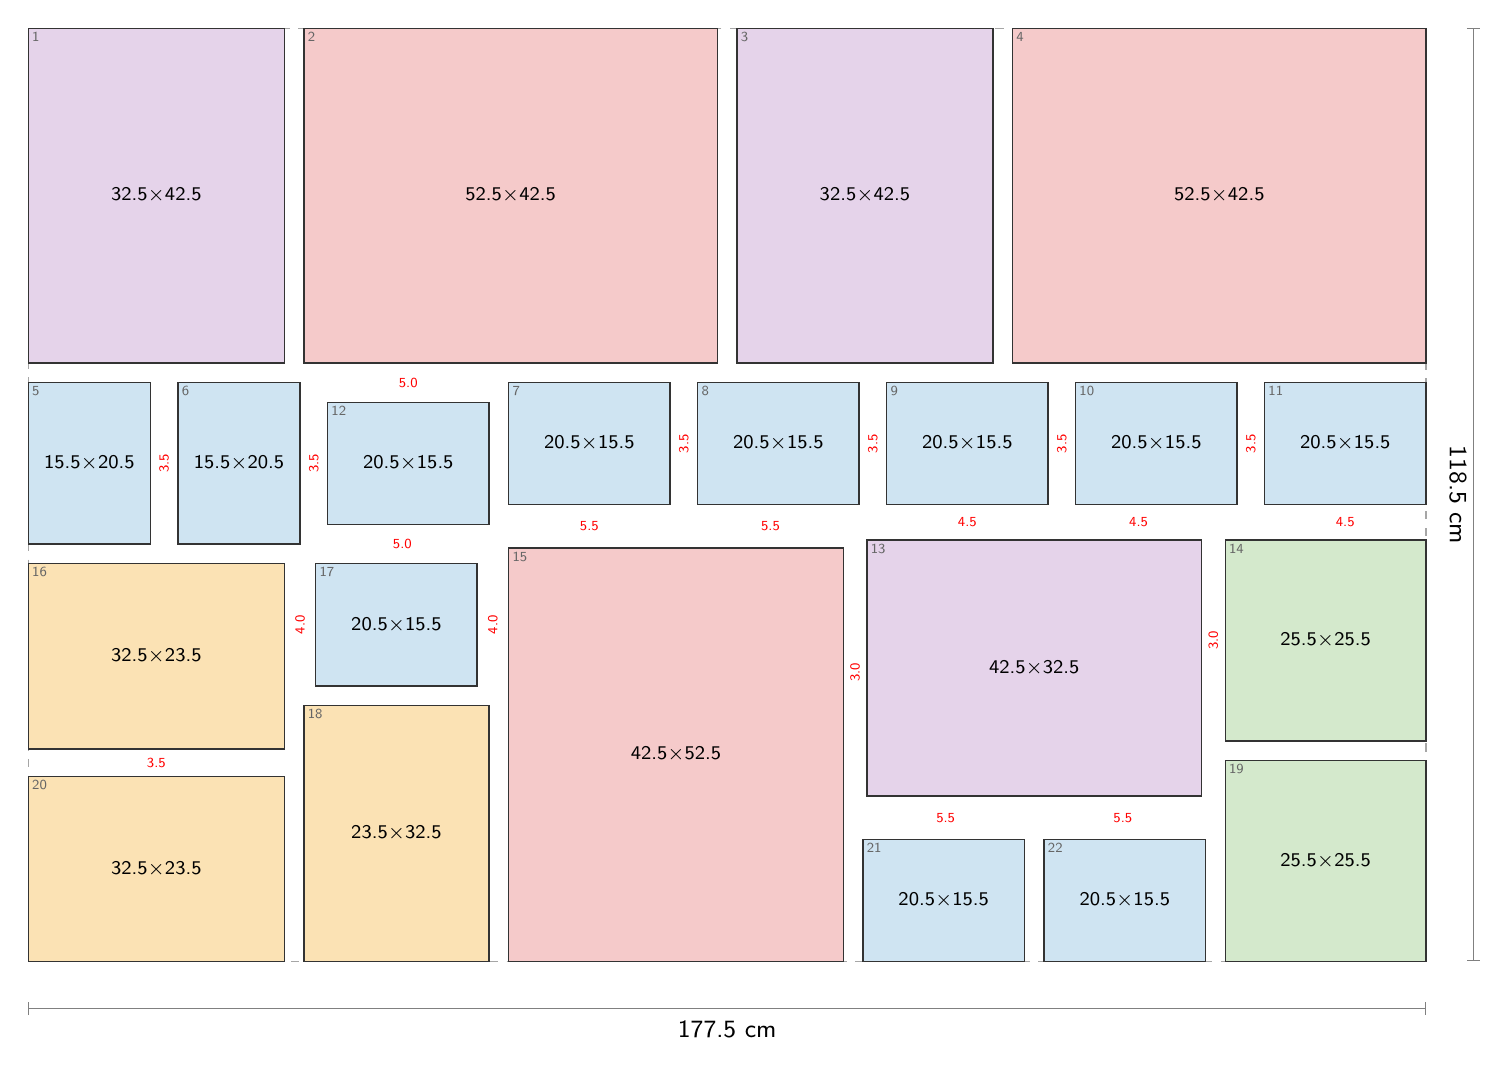
\begin{tikzpicture}[x=1mm, y=-1mm]
\draw[gray!70, dashed, line width=0.4pt] (0,0) rectangle (177.50,118.50);
\filldraw[fill=ft3, draw=black!80, line width=0.5pt] (0.00,0.00) rectangle (32.50,42.50);
\node[align=center, inner sep=0pt] at (16.25,21.25) {\scriptsize 32.5$\times$42.5};
\node[anchor=north west, inner sep=1.2pt, font=\tiny, text=black!60] at (0.00,0.00) {1};
\filldraw[fill=ft4, draw=black!80, line width=0.5pt] (35.00,0.00) rectangle (87.50,42.50);
\node[align=center, inner sep=0pt] at (61.25,21.25) {\scriptsize 52.5$\times$42.5};
\node[anchor=north west, inner sep=1.2pt, font=\tiny, text=black!60] at (35.00,0.00) {2};
\filldraw[fill=ft3, draw=black!80, line width=0.5pt] (90.00,0.00) rectangle (122.50,42.50);
\node[align=center, inner sep=0pt] at (106.25,21.25) {\scriptsize 32.5$\times$42.5};
\node[anchor=north west, inner sep=1.2pt, font=\tiny, text=black!60] at (90.00,0.00) {3};
\filldraw[fill=ft4, draw=black!80, line width=0.5pt] (125.00,0.00) rectangle (177.50,42.50);
\node[align=center, inner sep=0pt] at (151.25,21.25) {\scriptsize 52.5$\times$42.5};
\node[anchor=north west, inner sep=1.2pt, font=\tiny, text=black!60] at (125.00,0.00) {4};
\filldraw[fill=ft0, draw=black!80, line width=0.5pt] (0.00,45.00) rectangle (15.50,65.50);
\node[align=center, inner sep=0pt] at (7.75,55.25) {\scriptsize 15.5$\times$20.5};
\node[anchor=north west, inner sep=1.2pt, font=\tiny, text=black!60] at (0.00,45.00) {5};
\filldraw[fill=ft0, draw=black!80, line width=0.5pt] (19.00,45.00) rectangle (34.50,65.50);
\node[align=center, inner sep=0pt] at (26.75,55.25) {\scriptsize 15.5$\times$20.5};
\node[anchor=north west, inner sep=1.2pt, font=\tiny, text=black!60] at (19.00,45.00) {6};
\filldraw[fill=ft0, draw=black!80, line width=0.5pt] (61.00,45.00) rectangle (81.50,60.50);
\node[align=center, inner sep=0pt] at (71.25,52.75) {\scriptsize 20.5$\times$15.5};
\node[anchor=north west, inner sep=1.2pt, font=\tiny, text=black!60] at (61.00,45.00) {7};
\filldraw[fill=ft0, draw=black!80, line width=0.5pt] (85.00,45.00) rectangle (105.50,60.50);
\node[align=center, inner sep=0pt] at (95.25,52.75) {\scriptsize 20.5$\times$15.5};
\node[anchor=north west, inner sep=1.2pt, font=\tiny, text=black!60] at (85.00,45.00) {8};
\filldraw[fill=ft0, draw=black!80, line width=0.5pt] (109.00,45.00) rectangle (129.50,60.50);
\node[align=center, inner sep=0pt] at (119.25,52.75) {\scriptsize 20.5$\times$15.5};
\node[anchor=north west, inner sep=1.2pt, font=\tiny, text=black!60] at (109.00,45.00) {9};
\filldraw[fill=ft0, draw=black!80, line width=0.5pt] (133.00,45.00) rectangle (153.50,60.50);
\node[align=center, inner sep=0pt] at (143.25,52.75) {\scriptsize 20.5$\times$15.5};
\node[anchor=north west, inner sep=1.2pt, font=\tiny, text=black!60] at (133.00,45.00) {10};
\filldraw[fill=ft0, draw=black!80, line width=0.5pt] (157.00,45.00) rectangle (177.50,60.50);
\node[align=center, inner sep=0pt] at (167.25,52.75) {\scriptsize 20.5$\times$15.5};
\node[anchor=north west, inner sep=1.2pt, font=\tiny, text=black!60] at (157.00,45.00) {11};
\filldraw[fill=ft0, draw=black!80, line width=0.5pt] (38.00,47.50) rectangle (58.50,63.00);
\node[align=center, inner sep=0pt] at (48.25,55.25) {\scriptsize 20.5$\times$15.5};
\node[anchor=north west, inner sep=1.2pt, font=\tiny, text=black!60] at (38.00,47.50) {12};
\filldraw[fill=ft3, draw=black!80, line width=0.5pt] (106.50,65.00) rectangle (149.00,97.50);
\node[align=center, inner sep=0pt] at (127.75,81.25) {\scriptsize 42.5$\times$32.5};
\node[anchor=north west, inner sep=1.2pt, font=\tiny, text=black!60] at (106.50,65.00) {13};
\filldraw[fill=ft2, draw=black!80, line width=0.5pt] (152.00,65.00) rectangle (177.50,90.50);
\node[align=center, inner sep=0pt] at (164.75,77.75) {\scriptsize 25.5$\times$25.5};
\node[anchor=north west, inner sep=1.2pt, font=\tiny, text=black!60] at (152.00,65.00) {14};
\filldraw[fill=ft4, draw=black!80, line width=0.5pt] (61.00,66.00) rectangle (103.50,118.50);
\node[align=center, inner sep=0pt] at (82.25,92.25) {\scriptsize 42.5$\times$52.5};
\node[anchor=north west, inner sep=1.2pt, font=\tiny, text=black!60] at (61.00,66.00) {15};
\filldraw[fill=ft1, draw=black!80, line width=0.5pt] (0.00,68.00) rectangle (32.50,91.50);
\node[align=center, inner sep=0pt] at (16.25,79.75) {\scriptsize 32.5$\times$23.5};
\node[anchor=north west, inner sep=1.2pt, font=\tiny, text=black!60] at (0.00,68.00) {16};
\filldraw[fill=ft0, draw=black!80, line width=0.5pt] (36.50,68.00) rectangle (57.00,83.50);
\node[align=center, inner sep=0pt] at (46.75,75.75) {\scriptsize 20.5$\times$15.5};
\node[anchor=north west, inner sep=1.2pt, font=\tiny, text=black!60] at (36.50,68.00) {17};
\filldraw[fill=ft1, draw=black!80, line width=0.5pt] (35.00,86.00) rectangle (58.50,118.50);
\node[align=center, inner sep=0pt] at (46.75,102.25) {\scriptsize 23.5$\times$32.5};
\node[anchor=north west, inner sep=1.2pt, font=\tiny, text=black!60] at (35.00,86.00) {18};
\filldraw[fill=ft2, draw=black!80, line width=0.5pt] (152.00,93.00) rectangle (177.50,118.50);
\node[align=center, inner sep=0pt] at (164.75,105.75) {\scriptsize 25.5$\times$25.5};
\node[anchor=north west, inner sep=1.2pt, font=\tiny, text=black!60] at (152.00,93.00) {19};
\filldraw[fill=ft1, draw=black!80, line width=0.5pt] (0.00,95.00) rectangle (32.50,118.50);
\node[align=center, inner sep=0pt] at (16.25,106.75) {\scriptsize 32.5$\times$23.5};
\node[anchor=north west, inner sep=1.2pt, font=\tiny, text=black!60] at (0.00,95.00) {20};
\filldraw[fill=ft0, draw=black!80, line width=0.5pt] (106.00,103.00) rectangle (126.50,118.50);
\node[align=center, inner sep=0pt] at (116.25,110.75) {\scriptsize 20.5$\times$15.5};
\node[anchor=north west, inner sep=1.2pt, font=\tiny, text=black!60] at (106.00,103.00) {21};
\filldraw[fill=ft0, draw=black!80, line width=0.5pt] (129.00,103.00) rectangle (149.50,118.50);
\node[align=center, inner sep=0pt] at (139.25,110.75) {\scriptsize 20.5$\times$15.5};
\node[anchor=north west, inner sep=1.2pt, font=\tiny, text=black!60] at (129.00,103.00) {22};
\node[font=\tiny, text=red, fill=white, inner sep=0.3pt] at (48.25,45.00) {5.0};
\node[font=\tiny, text=red, fill=white, inner sep=0.3pt, rotate=90] at (17.25,55.25) {3.5};
\node[font=\tiny, text=red, fill=white, inner sep=0.3pt, rotate=90] at (36.25,55.25) {3.5};
\node[font=\tiny, text=red, fill=white, inner sep=0.3pt, rotate=90] at (83.25,52.75) {3.5};
\node[font=\tiny, text=red, fill=white, inner sep=0.3pt] at (71.25,63.25) {5.5};
\node[font=\tiny, text=red, fill=white, inner sep=0.3pt, rotate=90] at (107.25,52.75) {3.5};
\node[font=\tiny, text=red, fill=white, inner sep=0.3pt] at (94.25,63.25) {5.5};
\node[font=\tiny, text=red, fill=white, inner sep=0.3pt, rotate=90] at (131.25,52.75) {3.5};
\node[font=\tiny, text=red, fill=white, inner sep=0.3pt] at (119.25,62.75) {4.5};
\node[font=\tiny, text=red, fill=white, inner sep=0.3pt, rotate=90] at (155.25,52.75) {3.5};
\node[font=\tiny, text=red, fill=white, inner sep=0.3pt] at (141.00,62.75) {4.5};
\node[font=\tiny, text=red, fill=white, inner sep=0.3pt] at (167.25,62.75) {4.5};
\node[font=\tiny, text=red, fill=white, inner sep=0.3pt] at (47.50,65.50) {5.0};
\node[font=\tiny, text=red, fill=white, inner sep=0.3pt, rotate=90] at (150.50,77.75) {3.0};
\node[font=\tiny, text=red, fill=white, inner sep=0.3pt] at (116.50,100.25) {5.5};
\node[font=\tiny, text=red, fill=white, inner sep=0.3pt] at (139.00,100.25) {5.5};
\node[font=\tiny, text=red, fill=white, inner sep=0.3pt, rotate=90] at (105.00,81.75) {3.0};
\node[font=\tiny, text=red, fill=white, inner sep=0.3pt, rotate=90] at (34.50,75.75) {4.0};
\node[font=\tiny, text=red, fill=white, inner sep=0.3pt] at (16.25,93.25) {3.5};
\node[font=\tiny, text=red, fill=white, inner sep=0.3pt, rotate=90] at (59.00,75.75) {4.0};
\draw[Bar-Bar, gray] (0,124.50) -- (177.50,124.50) node[midway, below=1pt, font=\small, text=black] {177.5 cm};
\draw[Bar-Bar, gray] (183.50,0) -- (183.50,118.50) node[midway, right=1pt, font=\small, text=black, rotate=-90, anchor=north] {118.5 cm};
\end{tikzpicture}\\[4pt]
{\scriptsize Scale 1:10 (1 mm = 1 cm). Red numbers mark gaps that deviate from the nominal gap by more than 0.25 cm. Small grey numbers index the coordinate table.}
\end{minipage}\hfill
\begin{minipage}[t]{0.25\textwidth}\vspace{0pt}
\small
\begin{tabular}{@{}l l@{}}
\toprule
Outer size & 177.5 $\times$ 118.5 cm \\
Nominal gap & 2.5 cm \\
Actual gaps & 2.5 -- 5.5 cm \\
Max.\ deviation & 3.0 cm \\
Mean deviation & 0.83 cm \\
Border notches & right 4 cm \\
Corners filled & 4 / 4 \\
Frames used & 22 of 28 \\
Large frames & {\scriptsize 3, not touching, min.\ dist.\ 74 cm} \\
Entropy & 0.72 \\
\quad {\scriptsize mix / variety} & {\scriptsize 0.85 / 0.70} \\
\quad {\scriptsize stagger / lines} & {\scriptsize 0.58 / 0.75 (2 through)} \\
\bottomrule
\end{tabular}

\vspace{8pt}
\scriptsize
\begin{tabular}{@{}c l l r r@{}}
\toprule
 & outer w $\times$ h (cm) &  & used & have \\
\midrule
\tikz[baseline=-0.6ex]\fill[ft0,draw=black!60] (0,0) rectangle (1.2ex,1.2ex); & 20.5$\times$15.5 & L & 9 & 9 \\
\tikz[baseline=-0.6ex]\fill[ft0,draw=black!60] (0,0) rectangle (1.2ex,1.2ex); & 15.5$\times$20.5 & P & 2 & 2 \\
\tikz[baseline=-0.6ex]\fill[ft3,draw=black!60] (0,0) rectangle (1.2ex,1.2ex); & 32.5$\times$42.5 & P & 2 & 2 \\
\tikz[baseline=-0.6ex]\fill[ft3,draw=black!60] (0,0) rectangle (1.2ex,1.2ex); & 42.5$\times$32.5 & L & 1 & 1 \\
\tikz[baseline=-0.6ex]\fill[ft1,draw=black!60] (0,0) rectangle (1.2ex,1.2ex); & 32.5$\times$23.5 & L & 2 & 5 \\
\tikz[baseline=-0.6ex]\fill[ft1,draw=black!60] (0,0) rectangle (1.2ex,1.2ex); & 23.5$\times$32.5 & P & 1 & 1 \\
\tikz[baseline=-0.6ex]\fill[ft2,draw=black!60] (0,0) rectangle (1.2ex,1.2ex); & 25.5$\times$25.5 &  & 2 & 5 \\
\tikz[baseline=-0.6ex]\fill[ft4,draw=black!60] (0,0) rectangle (1.2ex,1.2ex); & 42.5$\times$52.5 & P & 1 & 1 \\
\tikz[baseline=-0.6ex]\fill[ft4,draw=black!60] (0,0) rectangle (1.2ex,1.2ex); & 52.5$\times$42.5 & L & 2 & 2 \\
\bottomrule
\end{tabular}

\vspace{8pt}
{\bfseries Positions} (top-left corner, cm)\\[2pt]
\tiny
\begin{tabular}{@{}r l r r@{}}
\toprule
\# & frame w $\times$ h & x & y \\
\midrule
1 & 32.5 $\times$ 42.5 & 0.0 & 0.0 \\
2 & 52.5 $\times$ 42.5 & 35.0 & 0.0 \\
3 & 32.5 $\times$ 42.5 & 90.0 & 0.0 \\
4 & 52.5 $\times$ 42.5 & 125.0 & 0.0 \\
5 & 15.5 $\times$ 20.5 & 0.0 & 45.0 \\
6 & 15.5 $\times$ 20.5 & 19.0 & 45.0 \\
7 & 20.5 $\times$ 15.5 & 61.0 & 45.0 \\
8 & 20.5 $\times$ 15.5 & 85.0 & 45.0 \\
9 & 20.5 $\times$ 15.5 & 109.0 & 45.0 \\
10 & 20.5 $\times$ 15.5 & 133.0 & 45.0 \\
11 & 20.5 $\times$ 15.5 & 157.0 & 45.0 \\
12 & 20.5 $\times$ 15.5 & 38.0 & 47.5 \\
13 & 42.5 $\times$ 32.5 & 106.5 & 65.0 \\
14 & 25.5 $\times$ 25.5 & 152.0 & 65.0 \\
15 & 42.5 $\times$ 52.5 & 61.0 & 66.0 \\
16 & 32.5 $\times$ 23.5 & 0.0 & 68.0 \\
17 & 20.5 $\times$ 15.5 & 36.5 & 68.0 \\
18 & 23.5 $\times$ 32.5 & 35.0 & 86.0 \\
19 & 25.5 $\times$ 25.5 & 152.0 & 93.0 \\
20 & 32.5 $\times$ 23.5 & 0.0 & 95.0 \\
21 & 20.5 $\times$ 15.5 & 106.0 & 103.0 \\
22 & 20.5 $\times$ 15.5 & 129.0 & 103.0 \\
\bottomrule
\end{tabular}
\end{minipage}
\clearpage

\begin{minipage}[t]{0.74\textwidth}\vspace{0pt}
{\LARGE\bfseries Layout 13}\hspace{1.5em}{\large 173.5 $\times$ 116.5 cm \quad gap 3 cm \quad 21 frames}\\[8pt]
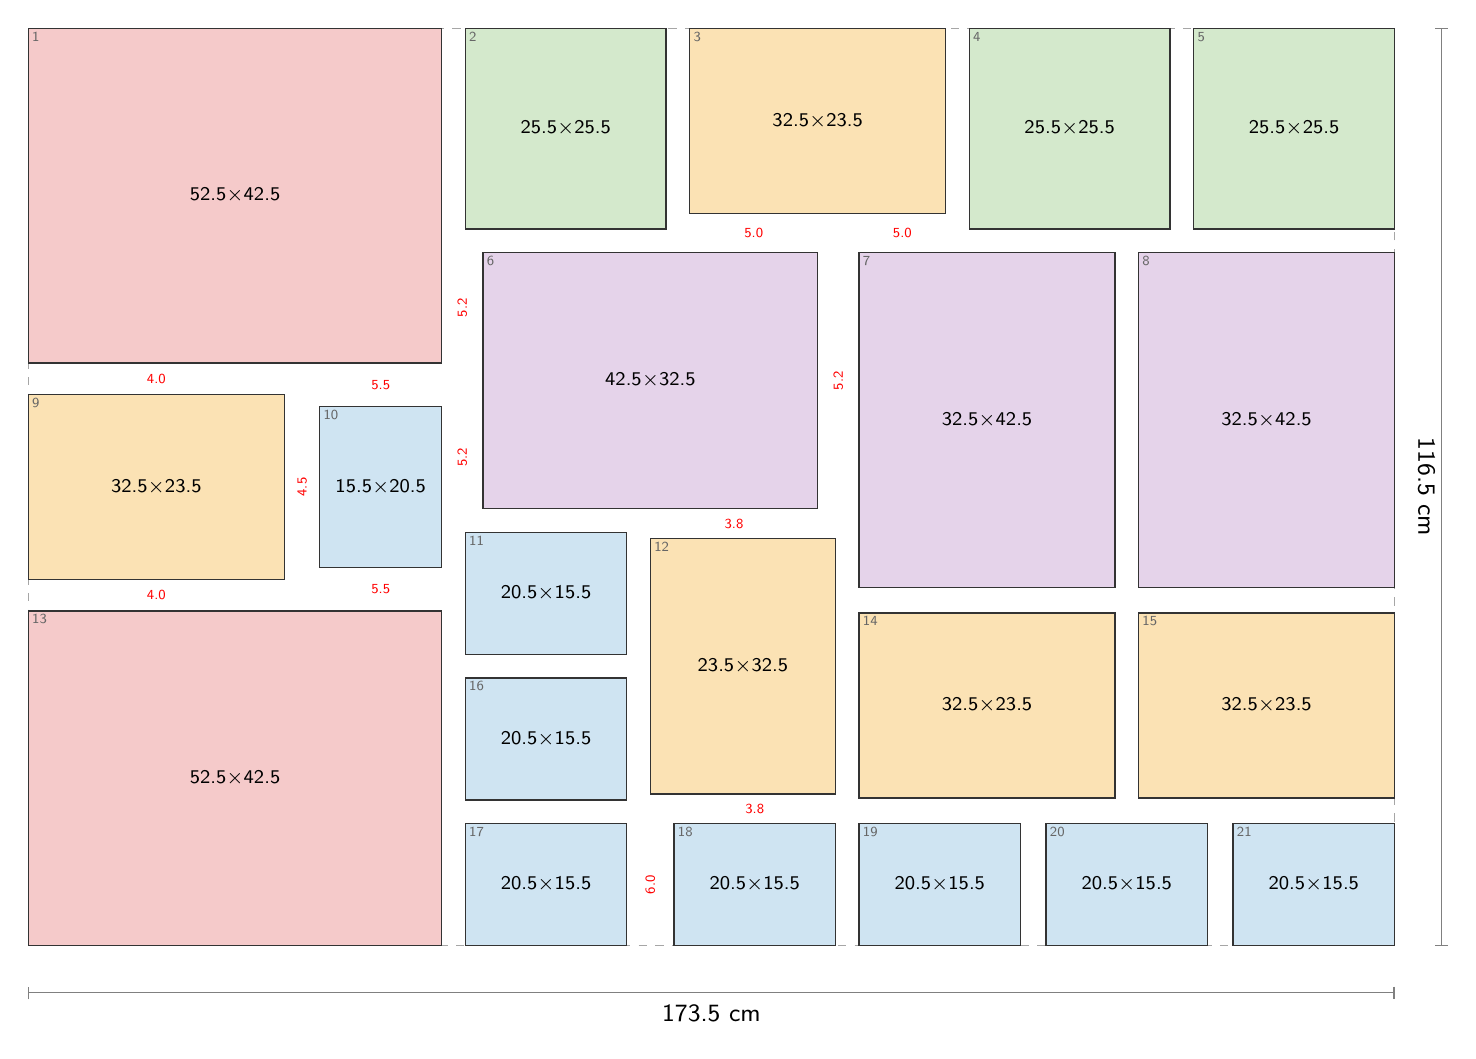
\begin{tikzpicture}[x=1mm, y=-1mm]
\draw[gray!70, dashed, line width=0.4pt] (0,0) rectangle (173.50,116.50);
\filldraw[fill=ft4, draw=black!80, line width=0.5pt] (0.00,0.00) rectangle (52.50,42.50);
\node[align=center, inner sep=0pt] at (26.25,21.25) {\scriptsize 52.5$\times$42.5};
\node[anchor=north west, inner sep=1.2pt, font=\tiny, text=black!60] at (0.00,0.00) {1};
\filldraw[fill=ft2, draw=black!80, line width=0.5pt] (55.50,0.00) rectangle (81.00,25.50);
\node[align=center, inner sep=0pt] at (68.25,12.75) {\scriptsize 25.5$\times$25.5};
\node[anchor=north west, inner sep=1.2pt, font=\tiny, text=black!60] at (55.50,0.00) {2};
\filldraw[fill=ft1, draw=black!80, line width=0.5pt] (84.00,0.00) rectangle (116.50,23.50);
\node[align=center, inner sep=0pt] at (100.25,11.75) {\scriptsize 32.5$\times$23.5};
\node[anchor=north west, inner sep=1.2pt, font=\tiny, text=black!60] at (84.00,0.00) {3};
\filldraw[fill=ft2, draw=black!80, line width=0.5pt] (119.50,0.00) rectangle (145.00,25.50);
\node[align=center, inner sep=0pt] at (132.25,12.75) {\scriptsize 25.5$\times$25.5};
\node[anchor=north west, inner sep=1.2pt, font=\tiny, text=black!60] at (119.50,0.00) {4};
\filldraw[fill=ft2, draw=black!80, line width=0.5pt] (148.00,0.00) rectangle (173.50,25.50);
\node[align=center, inner sep=0pt] at (160.75,12.75) {\scriptsize 25.5$\times$25.5};
\node[anchor=north west, inner sep=1.2pt, font=\tiny, text=black!60] at (148.00,0.00) {5};
\filldraw[fill=ft3, draw=black!80, line width=0.5pt] (57.75,28.50) rectangle (100.25,61.00);
\node[align=center, inner sep=0pt] at (79.00,44.75) {\scriptsize 42.5$\times$32.5};
\node[anchor=north west, inner sep=1.2pt, font=\tiny, text=black!60] at (57.75,28.50) {6};
\filldraw[fill=ft3, draw=black!80, line width=0.5pt] (105.50,28.50) rectangle (138.00,71.00);
\node[align=center, inner sep=0pt] at (121.75,49.75) {\scriptsize 32.5$\times$42.5};
\node[anchor=north west, inner sep=1.2pt, font=\tiny, text=black!60] at (105.50,28.50) {7};
\filldraw[fill=ft3, draw=black!80, line width=0.5pt] (141.00,28.50) rectangle (173.50,71.00);
\node[align=center, inner sep=0pt] at (157.25,49.75) {\scriptsize 32.5$\times$42.5};
\node[anchor=north west, inner sep=1.2pt, font=\tiny, text=black!60] at (141.00,28.50) {8};
\filldraw[fill=ft1, draw=black!80, line width=0.5pt] (0.00,46.50) rectangle (32.50,70.00);
\node[align=center, inner sep=0pt] at (16.25,58.25) {\scriptsize 32.5$\times$23.5};
\node[anchor=north west, inner sep=1.2pt, font=\tiny, text=black!60] at (0.00,46.50) {9};
\filldraw[fill=ft0, draw=black!80, line width=0.5pt] (37.00,48.00) rectangle (52.50,68.50);
\node[align=center, inner sep=0pt] at (44.75,58.25) {\scriptsize 15.5$\times$20.5};
\node[anchor=north west, inner sep=1.2pt, font=\tiny, text=black!60] at (37.00,48.00) {10};
\filldraw[fill=ft0, draw=black!80, line width=0.5pt] (55.50,64.00) rectangle (76.00,79.50);
\node[align=center, inner sep=0pt] at (65.75,71.75) {\scriptsize 20.5$\times$15.5};
\node[anchor=north west, inner sep=1.2pt, font=\tiny, text=black!60] at (55.50,64.00) {11};
\filldraw[fill=ft1, draw=black!80, line width=0.5pt] (79.00,64.75) rectangle (102.50,97.25);
\node[align=center, inner sep=0pt] at (90.75,81.00) {\scriptsize 23.5$\times$32.5};
\node[anchor=north west, inner sep=1.2pt, font=\tiny, text=black!60] at (79.00,64.75) {12};
\filldraw[fill=ft4, draw=black!80, line width=0.5pt] (0.00,74.00) rectangle (52.50,116.50);
\node[align=center, inner sep=0pt] at (26.25,95.25) {\scriptsize 52.5$\times$42.5};
\node[anchor=north west, inner sep=1.2pt, font=\tiny, text=black!60] at (0.00,74.00) {13};
\filldraw[fill=ft1, draw=black!80, line width=0.5pt] (105.50,74.25) rectangle (138.00,97.75);
\node[align=center, inner sep=0pt] at (121.75,86.00) {\scriptsize 32.5$\times$23.5};
\node[anchor=north west, inner sep=1.2pt, font=\tiny, text=black!60] at (105.50,74.25) {14};
\filldraw[fill=ft1, draw=black!80, line width=0.5pt] (141.00,74.25) rectangle (173.50,97.75);
\node[align=center, inner sep=0pt] at (157.25,86.00) {\scriptsize 32.5$\times$23.5};
\node[anchor=north west, inner sep=1.2pt, font=\tiny, text=black!60] at (141.00,74.25) {15};
\filldraw[fill=ft0, draw=black!80, line width=0.5pt] (55.50,82.50) rectangle (76.00,98.00);
\node[align=center, inner sep=0pt] at (65.75,90.25) {\scriptsize 20.5$\times$15.5};
\node[anchor=north west, inner sep=1.2pt, font=\tiny, text=black!60] at (55.50,82.50) {16};
\filldraw[fill=ft0, draw=black!80, line width=0.5pt] (55.50,101.00) rectangle (76.00,116.50);
\node[align=center, inner sep=0pt] at (65.75,108.75) {\scriptsize 20.5$\times$15.5};
\node[anchor=north west, inner sep=1.2pt, font=\tiny, text=black!60] at (55.50,101.00) {17};
\filldraw[fill=ft0, draw=black!80, line width=0.5pt] (82.00,101.00) rectangle (102.50,116.50);
\node[align=center, inner sep=0pt] at (92.25,108.75) {\scriptsize 20.5$\times$15.5};
\node[anchor=north west, inner sep=1.2pt, font=\tiny, text=black!60] at (82.00,101.00) {18};
\filldraw[fill=ft0, draw=black!80, line width=0.5pt] (105.50,101.00) rectangle (126.00,116.50);
\node[align=center, inner sep=0pt] at (115.75,108.75) {\scriptsize 20.5$\times$15.5};
\node[anchor=north west, inner sep=1.2pt, font=\tiny, text=black!60] at (105.50,101.00) {19};
\filldraw[fill=ft0, draw=black!80, line width=0.5pt] (129.25,101.00) rectangle (149.75,116.50);
\node[align=center, inner sep=0pt] at (139.50,108.75) {\scriptsize 20.5$\times$15.5};
\node[anchor=north west, inner sep=1.2pt, font=\tiny, text=black!60] at (129.25,101.00) {20};
\filldraw[fill=ft0, draw=black!80, line width=0.5pt] (153.00,101.00) rectangle (173.50,116.50);
\node[align=center, inner sep=0pt] at (163.25,108.75) {\scriptsize 20.5$\times$15.5};
\node[anchor=north west, inner sep=1.2pt, font=\tiny, text=black!60] at (153.00,101.00) {21};
\node[font=\tiny, text=red, fill=white, inner sep=0.3pt, rotate=90] at (55.12,35.50) {5.2};
\node[font=\tiny, text=red, fill=white, inner sep=0.3pt] at (16.25,44.50) {4.0};
\node[font=\tiny, text=red, fill=white, inner sep=0.3pt] at (44.75,45.25) {5.5};
\node[font=\tiny, text=red, fill=white, inner sep=0.3pt] at (92.12,26.00) {5.0};
\node[font=\tiny, text=red, fill=white, inner sep=0.3pt] at (111.00,26.00) {5.0};
\node[font=\tiny, text=red, fill=white, inner sep=0.3pt, rotate=90] at (102.88,44.75) {5.2};
\node[font=\tiny, text=red, fill=white, inner sep=0.3pt] at (89.62,62.88) {3.8};
\node[font=\tiny, text=red, fill=white, inner sep=0.3pt, rotate=90] at (34.75,58.25) {4.5};
\node[font=\tiny, text=red, fill=white, inner sep=0.3pt] at (16.25,72.00) {4.0};
\node[font=\tiny, text=red, fill=white, inner sep=0.3pt, rotate=90] at (55.12,54.50) {5.2};
\node[font=\tiny, text=red, fill=white, inner sep=0.3pt] at (44.75,71.25) {5.5};
\node[font=\tiny, text=red, fill=white, inner sep=0.3pt] at (92.25,99.12) {3.8};
\node[font=\tiny, text=red, fill=white, inner sep=0.3pt, rotate=90] at (79.00,108.75) {6.0};
\draw[Bar-Bar, gray] (0,122.50) -- (173.50,122.50) node[midway, below=1pt, font=\small, text=black] {173.5 cm};
\draw[Bar-Bar, gray] (179.50,0) -- (179.50,116.50) node[midway, right=1pt, font=\small, text=black, rotate=-90, anchor=north] {116.5 cm};
\end{tikzpicture}\\[4pt]
{\scriptsize Scale 1:10 (1 mm = 1 cm). Red numbers mark gaps that deviate from the nominal gap by more than 0.25 cm. Small grey numbers index the coordinate table.}
\end{minipage}\hfill
\begin{minipage}[t]{0.25\textwidth}\vspace{0pt}
\small
\begin{tabular}{@{}l l@{}}
\toprule
Outer size & 173.5 $\times$ 116.5 cm \\
Nominal gap & 3 cm \\
Actual gaps & 3.0 -- 6.0 cm \\
Max.\ deviation & 3.0 cm \\
Mean deviation & 0.63 cm \\
Border notches & bottom 6 cm \\
Corners filled & 4 / 4 \\
Frames used & 21 of 28 \\
Large frames & {\scriptsize 2, not touching, min.\ dist.\ 74 cm} \\
Entropy & 0.79 \\
\quad {\scriptsize mix / variety} & {\scriptsize 0.84 / 0.75} \\
\quad {\scriptsize stagger / lines} & {\scriptsize 0.56 / 1.00 (1 through)} \\
\bottomrule
\end{tabular}

\vspace{8pt}
\scriptsize
\begin{tabular}{@{}c l l r r@{}}
\toprule
 & outer w $\times$ h (cm) &  & used & have \\
\midrule
\tikz[baseline=-0.6ex]\fill[ft0,draw=black!60] (0,0) rectangle (1.2ex,1.2ex); & 20.5$\times$15.5 & L & 7 & 9 \\
\tikz[baseline=-0.6ex]\fill[ft0,draw=black!60] (0,0) rectangle (1.2ex,1.2ex); & 15.5$\times$20.5 & P & 1 & 2 \\
\tikz[baseline=-0.6ex]\fill[ft3,draw=black!60] (0,0) rectangle (1.2ex,1.2ex); & 32.5$\times$42.5 & P & 2 & 2 \\
\tikz[baseline=-0.6ex]\fill[ft3,draw=black!60] (0,0) rectangle (1.2ex,1.2ex); & 42.5$\times$32.5 & L & 1 & 1 \\
\tikz[baseline=-0.6ex]\fill[ft1,draw=black!60] (0,0) rectangle (1.2ex,1.2ex); & 32.5$\times$23.5 & L & 4 & 5 \\
\tikz[baseline=-0.6ex]\fill[ft1,draw=black!60] (0,0) rectangle (1.2ex,1.2ex); & 23.5$\times$32.5 & P & 1 & 1 \\
\tikz[baseline=-0.6ex]\fill[ft2,draw=black!60] (0,0) rectangle (1.2ex,1.2ex); & 25.5$\times$25.5 &  & 3 & 5 \\
\tikz[baseline=-0.6ex]\fill[ft4,draw=black!60] (0,0) rectangle (1.2ex,1.2ex); & 42.5$\times$52.5 & P & 0 & 1 \\
\tikz[baseline=-0.6ex]\fill[ft4,draw=black!60] (0,0) rectangle (1.2ex,1.2ex); & 52.5$\times$42.5 & L & 2 & 2 \\
\bottomrule
\end{tabular}

\vspace{8pt}
{\bfseries Positions} (top-left corner, cm)\\[2pt]
\tiny
\begin{tabular}{@{}r l r r@{}}
\toprule
\# & frame w $\times$ h & x & y \\
\midrule
1 & 52.5 $\times$ 42.5 & 0.0 & 0.0 \\
2 & 25.5 $\times$ 25.5 & 55.5 & 0.0 \\
3 & 32.5 $\times$ 23.5 & 84.0 & 0.0 \\
4 & 25.5 $\times$ 25.5 & 119.5 & 0.0 \\
5 & 25.5 $\times$ 25.5 & 148.0 & 0.0 \\
6 & 42.5 $\times$ 32.5 & 57.8 & 28.5 \\
7 & 32.5 $\times$ 42.5 & 105.5 & 28.5 \\
8 & 32.5 $\times$ 42.5 & 141.0 & 28.5 \\
9 & 32.5 $\times$ 23.5 & 0.0 & 46.5 \\
10 & 15.5 $\times$ 20.5 & 37.0 & 48.0 \\
11 & 20.5 $\times$ 15.5 & 55.5 & 64.0 \\
12 & 23.5 $\times$ 32.5 & 79.0 & 64.8 \\
13 & 52.5 $\times$ 42.5 & 0.0 & 74.0 \\
14 & 32.5 $\times$ 23.5 & 105.5 & 74.2 \\
15 & 32.5 $\times$ 23.5 & 141.0 & 74.2 \\
16 & 20.5 $\times$ 15.5 & 55.5 & 82.5 \\
17 & 20.5 $\times$ 15.5 & 55.5 & 101.0 \\
18 & 20.5 $\times$ 15.5 & 82.0 & 101.0 \\
19 & 20.5 $\times$ 15.5 & 105.5 & 101.0 \\
20 & 20.5 $\times$ 15.5 & 129.2 & 101.0 \\
21 & 20.5 $\times$ 15.5 & 153.0 & 101.0 \\
\bottomrule
\end{tabular}
\end{minipage}
\clearpage

\begin{minipage}[t]{0.74\textwidth}\vspace{0pt}
{\LARGE\bfseries Layout 14}\hspace{1.5em}{\large 176.0 $\times$ 125.0 cm \quad gap 2 cm \quad 20 frames}\\[8pt]
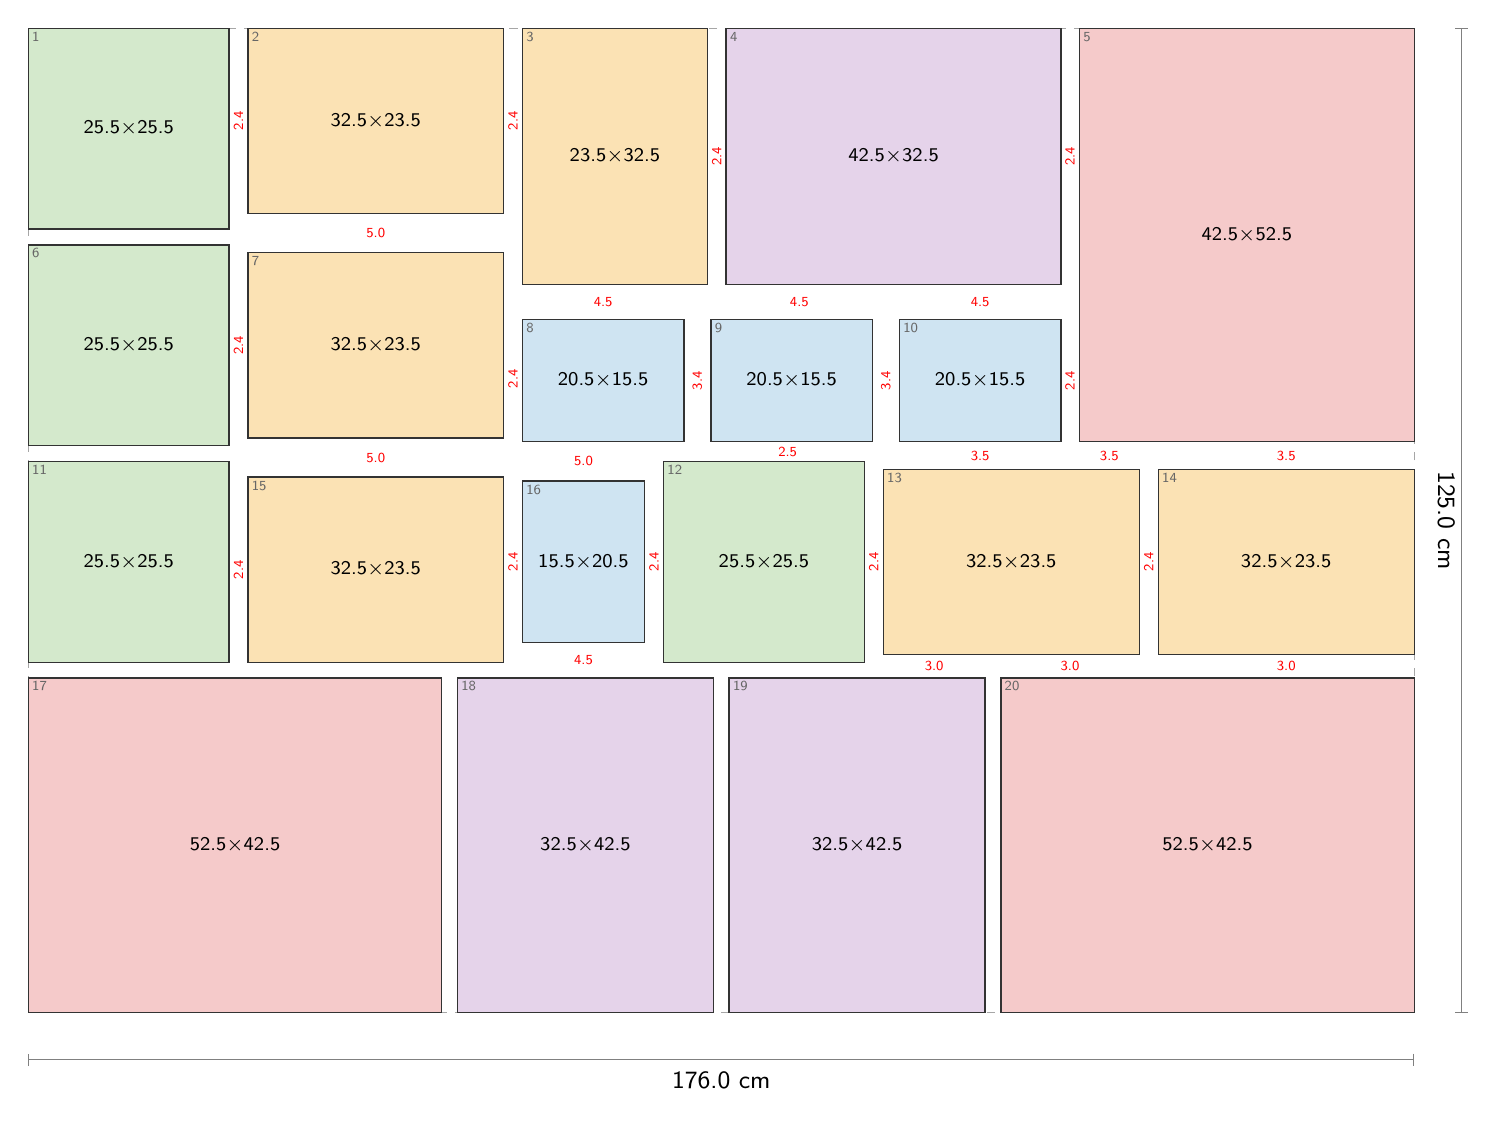
\begin{tikzpicture}[x=1mm, y=-1mm]
\draw[gray!70, dashed, line width=0.4pt] (0,0) rectangle (176.00,125.00);
\filldraw[fill=ft2, draw=black!80, line width=0.5pt] (0.00,0.00) rectangle (25.50,25.50);
\node[align=center, inner sep=0pt] at (12.75,12.75) {\scriptsize 25.5$\times$25.5};
\node[anchor=north west, inner sep=1.2pt, font=\tiny, text=black!60] at (0.00,0.00) {1};
\filldraw[fill=ft1, draw=black!80, line width=0.5pt] (27.88,0.00) rectangle (60.38,23.50);
\node[align=center, inner sep=0pt] at (44.12,11.75) {\scriptsize 32.5$\times$23.5};
\node[anchor=north west, inner sep=1.2pt, font=\tiny, text=black!60] at (27.88,0.00) {2};
\filldraw[fill=ft1, draw=black!80, line width=0.5pt] (62.75,0.00) rectangle (86.25,32.50);
\node[align=center, inner sep=0pt] at (74.50,16.25) {\scriptsize 23.5$\times$32.5};
\node[anchor=north west, inner sep=1.2pt, font=\tiny, text=black!60] at (62.75,0.00) {3};
\filldraw[fill=ft3, draw=black!80, line width=0.5pt] (88.62,0.00) rectangle (131.12,32.50);
\node[align=center, inner sep=0pt] at (109.88,16.25) {\scriptsize 42.5$\times$32.5};
\node[anchor=north west, inner sep=1.2pt, font=\tiny, text=black!60] at (88.62,0.00) {4};
\filldraw[fill=ft4, draw=black!80, line width=0.5pt] (133.50,0.00) rectangle (176.00,52.50);
\node[align=center, inner sep=0pt] at (154.75,26.25) {\scriptsize 42.5$\times$52.5};
\node[anchor=north west, inner sep=1.2pt, font=\tiny, text=black!60] at (133.50,0.00) {5};
\filldraw[fill=ft2, draw=black!80, line width=0.5pt] (0.00,27.50) rectangle (25.50,53.00);
\node[align=center, inner sep=0pt] at (12.75,40.25) {\scriptsize 25.5$\times$25.5};
\node[anchor=north west, inner sep=1.2pt, font=\tiny, text=black!60] at (0.00,27.50) {6};
\filldraw[fill=ft1, draw=black!80, line width=0.5pt] (27.88,28.50) rectangle (60.38,52.00);
\node[align=center, inner sep=0pt] at (44.12,40.25) {\scriptsize 32.5$\times$23.5};
\node[anchor=north west, inner sep=1.2pt, font=\tiny, text=black!60] at (27.88,28.50) {7};
\filldraw[fill=ft0, draw=black!80, line width=0.5pt] (62.75,37.00) rectangle (83.25,52.50);
\node[align=center, inner sep=0pt] at (73.00,44.75) {\scriptsize 20.5$\times$15.5};
\node[anchor=north west, inner sep=1.2pt, font=\tiny, text=black!60] at (62.75,37.00) {8};
\filldraw[fill=ft0, draw=black!80, line width=0.5pt] (86.69,37.00) rectangle (107.19,52.50);
\node[align=center, inner sep=0pt] at (96.94,44.75) {\scriptsize 20.5$\times$15.5};
\node[anchor=north west, inner sep=1.2pt, font=\tiny, text=black!60] at (86.69,37.00) {9};
\filldraw[fill=ft0, draw=black!80, line width=0.5pt] (110.62,37.00) rectangle (131.12,52.50);
\node[align=center, inner sep=0pt] at (120.88,44.75) {\scriptsize 20.5$\times$15.5};
\node[anchor=north west, inner sep=1.2pt, font=\tiny, text=black!60] at (110.62,37.00) {10};
\filldraw[fill=ft2, draw=black!80, line width=0.5pt] (0.00,55.00) rectangle (25.50,80.50);
\node[align=center, inner sep=0pt] at (12.75,67.75) {\scriptsize 25.5$\times$25.5};
\node[anchor=north west, inner sep=1.2pt, font=\tiny, text=black!60] at (0.00,55.00) {11};
\filldraw[fill=ft2, draw=black!80, line width=0.5pt] (80.67,55.00) rectangle (106.17,80.50);
\node[align=center, inner sep=0pt] at (93.42,67.75) {\scriptsize 25.5$\times$25.5};
\node[anchor=north west, inner sep=1.2pt, font=\tiny, text=black!60] at (80.67,55.00) {12};
\filldraw[fill=ft1, draw=black!80, line width=0.5pt] (108.58,56.00) rectangle (141.08,79.50);
\node[align=center, inner sep=0pt] at (124.83,67.75) {\scriptsize 32.5$\times$23.5};
\node[anchor=north west, inner sep=1.2pt, font=\tiny, text=black!60] at (108.58,56.00) {13};
\filldraw[fill=ft1, draw=black!80, line width=0.5pt] (143.50,56.00) rectangle (176.00,79.50);
\node[align=center, inner sep=0pt] at (159.75,67.75) {\scriptsize 32.5$\times$23.5};
\node[anchor=north west, inner sep=1.2pt, font=\tiny, text=black!60] at (143.50,56.00) {14};
\filldraw[fill=ft1, draw=black!80, line width=0.5pt] (27.88,57.00) rectangle (60.38,80.50);
\node[align=center, inner sep=0pt] at (44.12,68.75) {\scriptsize 32.5$\times$23.5};
\node[anchor=north west, inner sep=1.2pt, font=\tiny, text=black!60] at (27.88,57.00) {15};
\filldraw[fill=ft0, draw=black!80, line width=0.5pt] (62.75,57.50) rectangle (78.25,78.00);
\node[align=center, inner sep=0pt] at (70.50,67.75) {\scriptsize 15.5$\times$20.5};
\node[anchor=north west, inner sep=1.2pt, font=\tiny, text=black!60] at (62.75,57.50) {16};
\filldraw[fill=ft4, draw=black!80, line width=0.5pt] (0.00,82.50) rectangle (52.50,125.00);
\node[align=center, inner sep=0pt] at (26.25,103.75) {\scriptsize 52.5$\times$42.5};
\node[anchor=north west, inner sep=1.2pt, font=\tiny, text=black!60] at (0.00,82.50) {17};
\filldraw[fill=ft3, draw=black!80, line width=0.5pt] (54.50,82.50) rectangle (87.00,125.00);
\node[align=center, inner sep=0pt] at (70.75,103.75) {\scriptsize 32.5$\times$42.5};
\node[anchor=north west, inner sep=1.2pt, font=\tiny, text=black!60] at (54.50,82.50) {18};
\filldraw[fill=ft3, draw=black!80, line width=0.5pt] (89.00,82.50) rectangle (121.50,125.00);
\node[align=center, inner sep=0pt] at (105.25,103.75) {\scriptsize 32.5$\times$42.5};
\node[anchor=north west, inner sep=1.2pt, font=\tiny, text=black!60] at (89.00,82.50) {19};
\filldraw[fill=ft4, draw=black!80, line width=0.5pt] (123.50,82.50) rectangle (176.00,125.00);
\node[align=center, inner sep=0pt] at (149.75,103.75) {\scriptsize 52.5$\times$42.5};
\node[anchor=north west, inner sep=1.2pt, font=\tiny, text=black!60] at (123.50,82.50) {20};
\node[font=\tiny, text=red, fill=white, inner sep=0.3pt, rotate=90] at (26.69,11.75) {2.4};
\node[font=\tiny, text=red, fill=white, inner sep=0.3pt, rotate=90] at (61.56,11.75) {2.4};
\node[font=\tiny, text=red, fill=white, inner sep=0.3pt] at (44.12,26.00) {5.0};
\node[font=\tiny, text=red, fill=white, inner sep=0.3pt, rotate=90] at (87.44,16.25) {2.4};
\node[font=\tiny, text=red, fill=white, inner sep=0.3pt] at (73.00,34.75) {4.5};
\node[font=\tiny, text=red, fill=white, inner sep=0.3pt, rotate=90] at (132.31,16.25) {2.4};
\node[font=\tiny, text=red, fill=white, inner sep=0.3pt] at (97.91,34.75) {4.5};
\node[font=\tiny, text=red, fill=white, inner sep=0.3pt] at (120.88,34.75) {4.5};
\node[font=\tiny, text=red, fill=white, inner sep=0.3pt] at (137.29,54.25) {3.5};
\node[font=\tiny, text=red, fill=white, inner sep=0.3pt] at (159.75,54.25) {3.5};
\node[font=\tiny, text=red, fill=white, inner sep=0.3pt, rotate=90] at (26.69,40.25) {2.4};
\node[font=\tiny, text=red, fill=white, inner sep=0.3pt, rotate=90] at (61.56,44.50) {2.4};
\node[font=\tiny, text=red, fill=white, inner sep=0.3pt] at (44.12,54.50) {5.0};
\node[font=\tiny, text=red, fill=white, inner sep=0.3pt, rotate=90] at (84.97,44.75) {3.4};
\node[font=\tiny, text=red, fill=white, inner sep=0.3pt] at (70.50,55.00) {5.0};
\node[font=\tiny, text=red, fill=white, inner sep=0.3pt, rotate=90] at (108.91,44.75) {3.4};
\node[font=\tiny, text=red, fill=white, inner sep=0.3pt] at (96.43,53.75) {2.5};
\node[font=\tiny, text=red, fill=white, inner sep=0.3pt, rotate=90] at (132.31,44.75) {2.4};
\node[font=\tiny, text=red, fill=white, inner sep=0.3pt] at (120.88,54.25) {3.5};
\node[font=\tiny, text=red, fill=white, inner sep=0.3pt, rotate=90] at (26.69,68.75) {2.4};
\node[font=\tiny, text=red, fill=white, inner sep=0.3pt, rotate=90] at (107.38,67.75) {2.4};
\node[font=\tiny, text=red, fill=white, inner sep=0.3pt, rotate=90] at (142.29,67.75) {2.4};
\node[font=\tiny, text=red, fill=white, inner sep=0.3pt] at (115.04,81.00) {3.0};
\node[font=\tiny, text=red, fill=white, inner sep=0.3pt] at (132.29,81.00) {3.0};
\node[font=\tiny, text=red, fill=white, inner sep=0.3pt] at (159.75,81.00) {3.0};
\node[font=\tiny, text=red, fill=white, inner sep=0.3pt, rotate=90] at (61.56,67.75) {2.4};
\node[font=\tiny, text=red, fill=white, inner sep=0.3pt, rotate=90] at (79.46,67.75) {2.4};
\node[font=\tiny, text=red, fill=white, inner sep=0.3pt] at (70.50,80.25) {4.5};
\draw[Bar-Bar, gray] (0,131.00) -- (176.00,131.00) node[midway, below=1pt, font=\small, text=black] {176.0 cm};
\draw[Bar-Bar, gray] (182.00,0) -- (182.00,125.00) node[midway, right=1pt, font=\small, text=black, rotate=-90, anchor=north] {125.0 cm};
\end{tikzpicture}\\[4pt]
{\scriptsize Scale 1:10 (1 mm = 1 cm). Red numbers mark gaps that deviate from the nominal gap by more than 0.25 cm. Small grey numbers index the coordinate table.}
\end{minipage}\hfill
\begin{minipage}[t]{0.25\textwidth}\vspace{0pt}
\small
\begin{tabular}{@{}l l@{}}
\toprule
Outer size & 176.0 $\times$ 125.0 cm \\
Nominal gap & 2 cm \\
Actual gaps & 2.0 -- 5.0 cm \\
Max.\ deviation & 3.0 cm \\
Mean deviation & 0.91 cm \\
Border notches & right 4 cm \\
Corners filled & 4 / 4 \\
Frames used & 20 of 28 \\
Large frames & {\scriptsize 3, not touching, min.\ dist.\ 78 cm} \\
Entropy & 0.77 \\
\quad {\scriptsize mix / variety} & {\scriptsize 0.92 / 0.85} \\
\quad {\scriptsize stagger / lines} & {\scriptsize 0.56 / 0.75 (2 through)} \\
\bottomrule
\end{tabular}

\vspace{8pt}
\scriptsize
\begin{tabular}{@{}c l l r r@{}}
\toprule
 & outer w $\times$ h (cm) &  & used & have \\
\midrule
\tikz[baseline=-0.6ex]\fill[ft0,draw=black!60] (0,0) rectangle (1.2ex,1.2ex); & 20.5$\times$15.5 & L & 3 & 9 \\
\tikz[baseline=-0.6ex]\fill[ft0,draw=black!60] (0,0) rectangle (1.2ex,1.2ex); & 15.5$\times$20.5 & P & 1 & 2 \\
\tikz[baseline=-0.6ex]\fill[ft3,draw=black!60] (0,0) rectangle (1.2ex,1.2ex); & 32.5$\times$42.5 & P & 2 & 2 \\
\tikz[baseline=-0.6ex]\fill[ft3,draw=black!60] (0,0) rectangle (1.2ex,1.2ex); & 42.5$\times$32.5 & L & 1 & 1 \\
\tikz[baseline=-0.6ex]\fill[ft1,draw=black!60] (0,0) rectangle (1.2ex,1.2ex); & 32.5$\times$23.5 & L & 5 & 5 \\
\tikz[baseline=-0.6ex]\fill[ft1,draw=black!60] (0,0) rectangle (1.2ex,1.2ex); & 23.5$\times$32.5 & P & 1 & 1 \\
\tikz[baseline=-0.6ex]\fill[ft2,draw=black!60] (0,0) rectangle (1.2ex,1.2ex); & 25.5$\times$25.5 &  & 4 & 5 \\
\tikz[baseline=-0.6ex]\fill[ft4,draw=black!60] (0,0) rectangle (1.2ex,1.2ex); & 42.5$\times$52.5 & P & 1 & 1 \\
\tikz[baseline=-0.6ex]\fill[ft4,draw=black!60] (0,0) rectangle (1.2ex,1.2ex); & 52.5$\times$42.5 & L & 2 & 2 \\
\bottomrule
\end{tabular}

\vspace{8pt}
{\bfseries Positions} (top-left corner, cm)\\[2pt]
\tiny
\begin{tabular}{@{}r l r r@{}}
\toprule
\# & frame w $\times$ h & x & y \\
\midrule
1 & 25.5 $\times$ 25.5 & 0.0 & 0.0 \\
2 & 32.5 $\times$ 23.5 & 27.9 & 0.0 \\
3 & 23.5 $\times$ 32.5 & 62.8 & 0.0 \\
4 & 42.5 $\times$ 32.5 & 88.6 & 0.0 \\
5 & 42.5 $\times$ 52.5 & 133.5 & 0.0 \\
6 & 25.5 $\times$ 25.5 & 0.0 & 27.5 \\
7 & 32.5 $\times$ 23.5 & 27.9 & 28.5 \\
8 & 20.5 $\times$ 15.5 & 62.8 & 37.0 \\
9 & 20.5 $\times$ 15.5 & 86.7 & 37.0 \\
10 & 20.5 $\times$ 15.5 & 110.6 & 37.0 \\
11 & 25.5 $\times$ 25.5 & 0.0 & 55.0 \\
12 & 25.5 $\times$ 25.5 & 80.7 & 55.0 \\
13 & 32.5 $\times$ 23.5 & 108.6 & 56.0 \\
14 & 32.5 $\times$ 23.5 & 143.5 & 56.0 \\
15 & 32.5 $\times$ 23.5 & 27.9 & 57.0 \\
16 & 15.5 $\times$ 20.5 & 62.8 & 57.5 \\
17 & 52.5 $\times$ 42.5 & 0.0 & 82.5 \\
18 & 32.5 $\times$ 42.5 & 54.5 & 82.5 \\
19 & 32.5 $\times$ 42.5 & 89.0 & 82.5 \\
20 & 52.5 $\times$ 42.5 & 123.5 & 82.5 \\
\bottomrule
\end{tabular}
\end{minipage}
\clearpage

\begin{minipage}[t]{0.74\textwidth}\vspace{0pt}
{\LARGE\bfseries Layout 15}\hspace{1.5em}{\large 179.5 $\times$ 120.5 cm \quad gap 1.5 cm \quad 26 frames}\\[8pt]
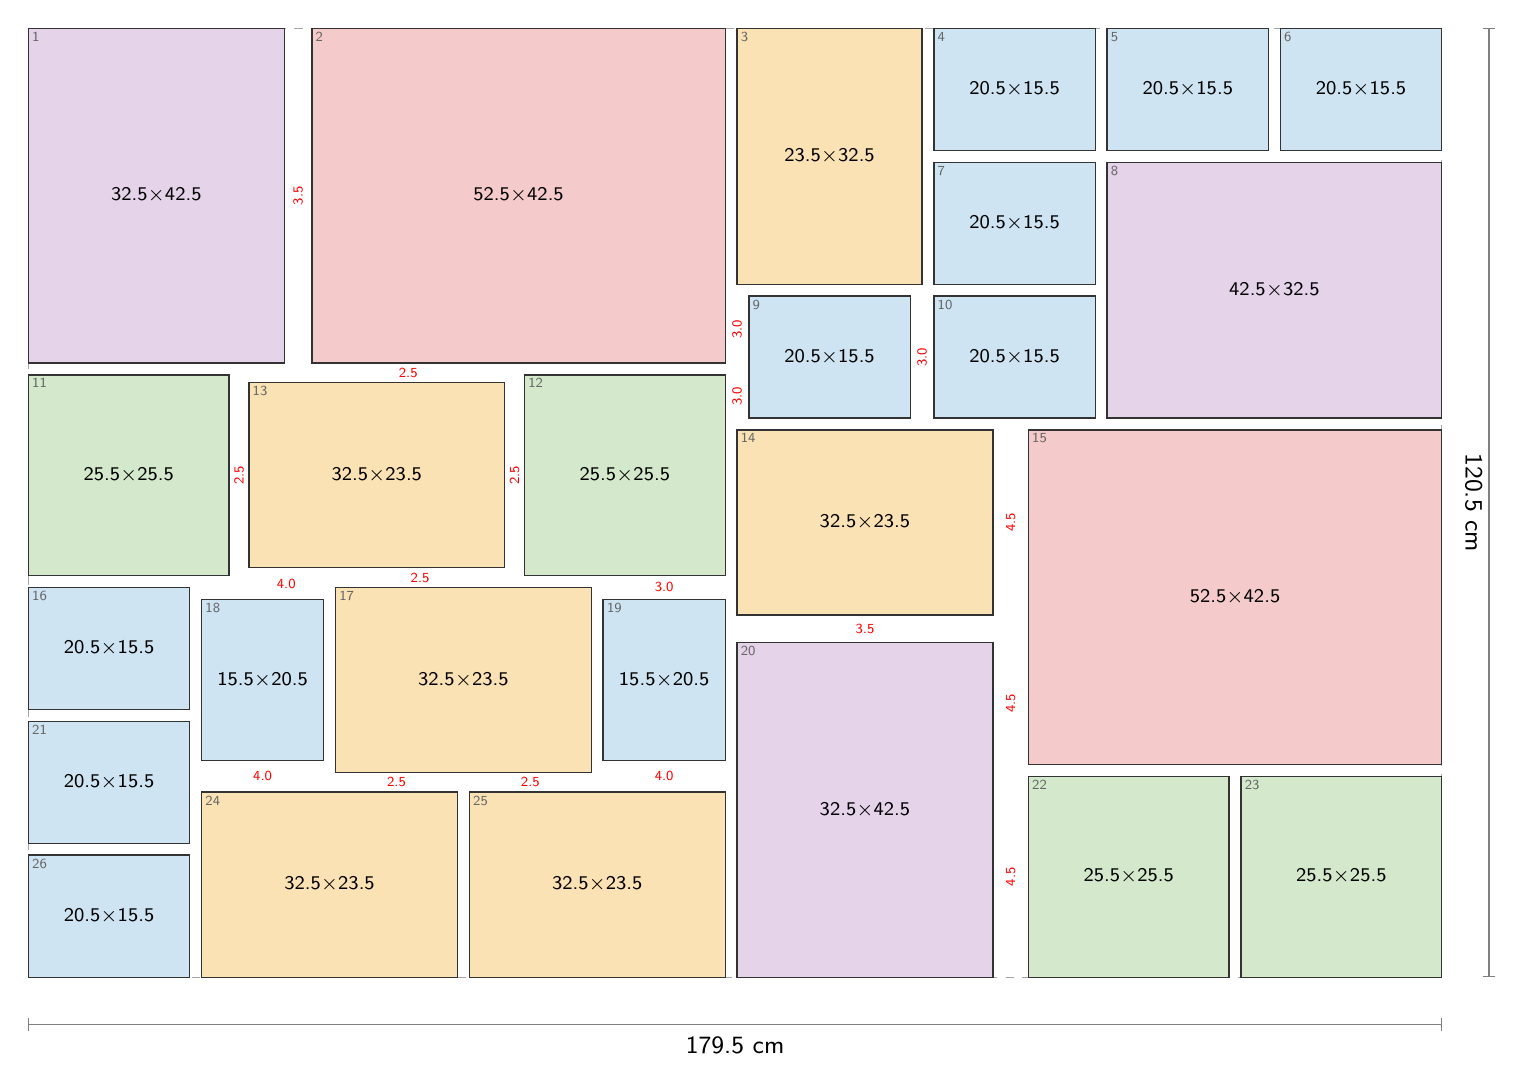
\begin{tikzpicture}[x=1mm, y=-1mm]
\draw[gray!70, dashed, line width=0.4pt] (0,0) rectangle (179.50,120.50);
\filldraw[fill=ft3, draw=black!80, line width=0.5pt] (0.00,0.00) rectangle (32.50,42.50);
\node[align=center, inner sep=0pt] at (16.25,21.25) {\scriptsize 32.5$\times$42.5};
\node[anchor=north west, inner sep=1.2pt, font=\tiny, text=black!60] at (0.00,0.00) {1};
\filldraw[fill=ft4, draw=black!80, line width=0.5pt] (36.00,0.00) rectangle (88.50,42.50);
\node[align=center, inner sep=0pt] at (62.25,21.25) {\scriptsize 52.5$\times$42.5};
\node[anchor=north west, inner sep=1.2pt, font=\tiny, text=black!60] at (36.00,0.00) {2};
\filldraw[fill=ft1, draw=black!80, line width=0.5pt] (90.00,0.00) rectangle (113.50,32.50);
\node[align=center, inner sep=0pt] at (101.75,16.25) {\scriptsize 23.5$\times$32.5};
\node[anchor=north west, inner sep=1.2pt, font=\tiny, text=black!60] at (90.00,0.00) {3};
\filldraw[fill=ft0, draw=black!80, line width=0.5pt] (115.00,0.00) rectangle (135.50,15.50);
\node[align=center, inner sep=0pt] at (125.25,7.75) {\scriptsize 20.5$\times$15.5};
\node[anchor=north west, inner sep=1.2pt, font=\tiny, text=black!60] at (115.00,0.00) {4};
\filldraw[fill=ft0, draw=black!80, line width=0.5pt] (137.00,0.00) rectangle (157.50,15.50);
\node[align=center, inner sep=0pt] at (147.25,7.75) {\scriptsize 20.5$\times$15.5};
\node[anchor=north west, inner sep=1.2pt, font=\tiny, text=black!60] at (137.00,0.00) {5};
\filldraw[fill=ft0, draw=black!80, line width=0.5pt] (159.00,0.00) rectangle (179.50,15.50);
\node[align=center, inner sep=0pt] at (169.25,7.75) {\scriptsize 20.5$\times$15.5};
\node[anchor=north west, inner sep=1.2pt, font=\tiny, text=black!60] at (159.00,0.00) {6};
\filldraw[fill=ft0, draw=black!80, line width=0.5pt] (115.00,17.00) rectangle (135.50,32.50);
\node[align=center, inner sep=0pt] at (125.25,24.75) {\scriptsize 20.5$\times$15.5};
\node[anchor=north west, inner sep=1.2pt, font=\tiny, text=black!60] at (115.00,17.00) {7};
\filldraw[fill=ft3, draw=black!80, line width=0.5pt] (137.00,17.00) rectangle (179.50,49.50);
\node[align=center, inner sep=0pt] at (158.25,33.25) {\scriptsize 42.5$\times$32.5};
\node[anchor=north west, inner sep=1.2pt, font=\tiny, text=black!60] at (137.00,17.00) {8};
\filldraw[fill=ft0, draw=black!80, line width=0.5pt] (91.50,34.00) rectangle (112.00,49.50);
\node[align=center, inner sep=0pt] at (101.75,41.75) {\scriptsize 20.5$\times$15.5};
\node[anchor=north west, inner sep=1.2pt, font=\tiny, text=black!60] at (91.50,34.00) {9};
\filldraw[fill=ft0, draw=black!80, line width=0.5pt] (115.00,34.00) rectangle (135.50,49.50);
\node[align=center, inner sep=0pt] at (125.25,41.75) {\scriptsize 20.5$\times$15.5};
\node[anchor=north west, inner sep=1.2pt, font=\tiny, text=black!60] at (115.00,34.00) {10};
\filldraw[fill=ft2, draw=black!80, line width=0.5pt] (0.00,44.00) rectangle (25.50,69.50);
\node[align=center, inner sep=0pt] at (12.75,56.75) {\scriptsize 25.5$\times$25.5};
\node[anchor=north west, inner sep=1.2pt, font=\tiny, text=black!60] at (0.00,44.00) {11};
\filldraw[fill=ft2, draw=black!80, line width=0.5pt] (63.00,44.00) rectangle (88.50,69.50);
\node[align=center, inner sep=0pt] at (75.75,56.75) {\scriptsize 25.5$\times$25.5};
\node[anchor=north west, inner sep=1.2pt, font=\tiny, text=black!60] at (63.00,44.00) {12};
\filldraw[fill=ft1, draw=black!80, line width=0.5pt] (28.00,45.00) rectangle (60.50,68.50);
\node[align=center, inner sep=0pt] at (44.25,56.75) {\scriptsize 32.5$\times$23.5};
\node[anchor=north west, inner sep=1.2pt, font=\tiny, text=black!60] at (28.00,45.00) {13};
\filldraw[fill=ft1, draw=black!80, line width=0.5pt] (90.00,51.00) rectangle (122.50,74.50);
\node[align=center, inner sep=0pt] at (106.25,62.75) {\scriptsize 32.5$\times$23.5};
\node[anchor=north west, inner sep=1.2pt, font=\tiny, text=black!60] at (90.00,51.00) {14};
\filldraw[fill=ft4, draw=black!80, line width=0.5pt] (127.00,51.00) rectangle (179.50,93.50);
\node[align=center, inner sep=0pt] at (153.25,72.25) {\scriptsize 52.5$\times$42.5};
\node[anchor=north west, inner sep=1.2pt, font=\tiny, text=black!60] at (127.00,51.00) {15};
\filldraw[fill=ft0, draw=black!80, line width=0.5pt] (0.00,71.00) rectangle (20.50,86.50);
\node[align=center, inner sep=0pt] at (10.25,78.75) {\scriptsize 20.5$\times$15.5};
\node[anchor=north west, inner sep=1.2pt, font=\tiny, text=black!60] at (0.00,71.00) {16};
\filldraw[fill=ft1, draw=black!80, line width=0.5pt] (39.00,71.00) rectangle (71.50,94.50);
\node[align=center, inner sep=0pt] at (55.25,82.75) {\scriptsize 32.5$\times$23.5};
\node[anchor=north west, inner sep=1.2pt, font=\tiny, text=black!60] at (39.00,71.00) {17};
\filldraw[fill=ft0, draw=black!80, line width=0.5pt] (22.00,72.50) rectangle (37.50,93.00);
\node[align=center, inner sep=0pt] at (29.75,82.75) {\scriptsize 15.5$\times$20.5};
\node[anchor=north west, inner sep=1.2pt, font=\tiny, text=black!60] at (22.00,72.50) {18};
\filldraw[fill=ft0, draw=black!80, line width=0.5pt] (73.00,72.50) rectangle (88.50,93.00);
\node[align=center, inner sep=0pt] at (80.75,82.75) {\scriptsize 15.5$\times$20.5};
\node[anchor=north west, inner sep=1.2pt, font=\tiny, text=black!60] at (73.00,72.50) {19};
\filldraw[fill=ft3, draw=black!80, line width=0.5pt] (90.00,78.00) rectangle (122.50,120.50);
\node[align=center, inner sep=0pt] at (106.25,99.25) {\scriptsize 32.5$\times$42.5};
\node[anchor=north west, inner sep=1.2pt, font=\tiny, text=black!60] at (90.00,78.00) {20};
\filldraw[fill=ft0, draw=black!80, line width=0.5pt] (0.00,88.00) rectangle (20.50,103.50);
\node[align=center, inner sep=0pt] at (10.25,95.75) {\scriptsize 20.5$\times$15.5};
\node[anchor=north west, inner sep=1.2pt, font=\tiny, text=black!60] at (0.00,88.00) {21};
\filldraw[fill=ft2, draw=black!80, line width=0.5pt] (127.00,95.00) rectangle (152.50,120.50);
\node[align=center, inner sep=0pt] at (139.75,107.75) {\scriptsize 25.5$\times$25.5};
\node[anchor=north west, inner sep=1.2pt, font=\tiny, text=black!60] at (127.00,95.00) {22};
\filldraw[fill=ft2, draw=black!80, line width=0.5pt] (154.00,95.00) rectangle (179.50,120.50);
\node[align=center, inner sep=0pt] at (166.75,107.75) {\scriptsize 25.5$\times$25.5};
\node[anchor=north west, inner sep=1.2pt, font=\tiny, text=black!60] at (154.00,95.00) {23};
\filldraw[fill=ft1, draw=black!80, line width=0.5pt] (22.00,97.00) rectangle (54.50,120.50);
\node[align=center, inner sep=0pt] at (38.25,108.75) {\scriptsize 32.5$\times$23.5};
\node[anchor=north west, inner sep=1.2pt, font=\tiny, text=black!60] at (22.00,97.00) {24};
\filldraw[fill=ft1, draw=black!80, line width=0.5pt] (56.00,97.00) rectangle (88.50,120.50);
\node[align=center, inner sep=0pt] at (72.25,108.75) {\scriptsize 32.5$\times$23.5};
\node[anchor=north west, inner sep=1.2pt, font=\tiny, text=black!60] at (56.00,97.00) {25};
\filldraw[fill=ft0, draw=black!80, line width=0.5pt] (0.00,105.00) rectangle (20.50,120.50);
\node[align=center, inner sep=0pt] at (10.25,112.75) {\scriptsize 20.5$\times$15.5};
\node[anchor=north west, inner sep=1.2pt, font=\tiny, text=black!60] at (0.00,105.00) {26};
\node[font=\tiny, text=red, fill=white, inner sep=0.3pt, rotate=90] at (34.25,21.25) {3.5};
\node[font=\tiny, text=red, fill=white, inner sep=0.3pt, rotate=90] at (90.00,38.25) {3.0};
\node[font=\tiny, text=red, fill=white, inner sep=0.3pt] at (48.25,43.75) {2.5};
\node[font=\tiny, text=red, fill=white, inner sep=0.3pt, rotate=90] at (113.50,41.75) {3.0};
\node[font=\tiny, text=red, fill=white, inner sep=0.3pt, rotate=90] at (26.75,56.75) {2.5};
\node[font=\tiny, text=red, fill=white, inner sep=0.3pt, rotate=90] at (90.00,46.75) {3.0};
\node[font=\tiny, text=red, fill=white, inner sep=0.3pt] at (80.75,71.00) {3.0};
\node[font=\tiny, text=red, fill=white, inner sep=0.3pt, rotate=90] at (61.75,56.75) {2.5};
\node[font=\tiny, text=red, fill=white, inner sep=0.3pt] at (49.75,69.75) {2.5};
\node[font=\tiny, text=red, fill=white, inner sep=0.3pt] at (32.75,70.50) {4.0};
\node[font=\tiny, text=red, fill=white, inner sep=0.3pt, rotate=90] at (124.75,62.75) {4.5};
\node[font=\tiny, text=red, fill=white, inner sep=0.3pt] at (106.25,76.25) {3.5};
\node[font=\tiny, text=red, fill=white, inner sep=0.3pt] at (46.75,95.75) {2.5};
\node[font=\tiny, text=red, fill=white, inner sep=0.3pt] at (63.75,95.75) {2.5};
\node[font=\tiny, text=red, fill=white, inner sep=0.3pt] at (29.75,95.00) {4.0};
\node[font=\tiny, text=red, fill=white, inner sep=0.3pt] at (80.75,95.00) {4.0};
\node[font=\tiny, text=red, fill=white, inner sep=0.3pt, rotate=90] at (124.75,85.75) {4.5};
\node[font=\tiny, text=red, fill=white, inner sep=0.3pt, rotate=90] at (124.75,107.75) {4.5};
\draw[Bar-Bar, gray] (0,126.50) -- (179.50,126.50) node[midway, below=1pt, font=\small, text=black] {179.5 cm};
\draw[Bar-Bar, gray] (185.50,0) -- (185.50,120.50) node[midway, right=1pt, font=\small, text=black, rotate=-90, anchor=north] {120.5 cm};
\end{tikzpicture}\\[4pt]
{\scriptsize Scale 1:10 (1 mm = 1 cm). Red numbers mark gaps that deviate from the nominal gap by more than 0.25 cm. Small grey numbers index the coordinate table.}
\end{minipage}\hfill
\begin{minipage}[t]{0.25\textwidth}\vspace{0pt}
\small
\begin{tabular}{@{}l l@{}}
\toprule
Outer size & 179.5 $\times$ 120.5 cm \\
Nominal gap & 1.5 cm \\
Actual gaps & 1.5 -- 4.5 cm \\
Max.\ deviation & 3.0 cm \\
Mean deviation & 0.61 cm \\
Border notches & top 4 cm, bottom 4 cm \\
Corners filled & 4 / 4 \\
Frames used & 26 of 28 \\
Large frames & {\scriptsize 2, not touching, min.\ dist.\ 104 cm} \\
Entropy & 0.77 \\
\quad {\scriptsize mix / variety} & {\scriptsize 0.83 / 0.73} \\
\quad {\scriptsize stagger / lines} & {\scriptsize 0.54 / 1.00 (1 through)} \\
\bottomrule
\end{tabular}

\vspace{8pt}
\scriptsize
\begin{tabular}{@{}c l l r r@{}}
\toprule
 & outer w $\times$ h (cm) &  & used & have \\
\midrule
\tikz[baseline=-0.6ex]\fill[ft0,draw=black!60] (0,0) rectangle (1.2ex,1.2ex); & 20.5$\times$15.5 & L & 9 & 9 \\
\tikz[baseline=-0.6ex]\fill[ft0,draw=black!60] (0,0) rectangle (1.2ex,1.2ex); & 15.5$\times$20.5 & P & 2 & 2 \\
\tikz[baseline=-0.6ex]\fill[ft3,draw=black!60] (0,0) rectangle (1.2ex,1.2ex); & 32.5$\times$42.5 & P & 2 & 2 \\
\tikz[baseline=-0.6ex]\fill[ft3,draw=black!60] (0,0) rectangle (1.2ex,1.2ex); & 42.5$\times$32.5 & L & 1 & 1 \\
\tikz[baseline=-0.6ex]\fill[ft1,draw=black!60] (0,0) rectangle (1.2ex,1.2ex); & 32.5$\times$23.5 & L & 5 & 5 \\
\tikz[baseline=-0.6ex]\fill[ft1,draw=black!60] (0,0) rectangle (1.2ex,1.2ex); & 23.5$\times$32.5 & P & 1 & 1 \\
\tikz[baseline=-0.6ex]\fill[ft2,draw=black!60] (0,0) rectangle (1.2ex,1.2ex); & 25.5$\times$25.5 &  & 4 & 5 \\
\tikz[baseline=-0.6ex]\fill[ft4,draw=black!60] (0,0) rectangle (1.2ex,1.2ex); & 42.5$\times$52.5 & P & 0 & 1 \\
\tikz[baseline=-0.6ex]\fill[ft4,draw=black!60] (0,0) rectangle (1.2ex,1.2ex); & 52.5$\times$42.5 & L & 2 & 2 \\
\bottomrule
\end{tabular}

\vspace{8pt}
{\bfseries Positions} (top-left corner, cm)\\[2pt]
\tiny
\begin{tabular}{@{}r l r r@{}}
\toprule
\# & frame w $\times$ h & x & y \\
\midrule
1 & 32.5 $\times$ 42.5 & 0.0 & 0.0 \\
2 & 52.5 $\times$ 42.5 & 36.0 & 0.0 \\
3 & 23.5 $\times$ 32.5 & 90.0 & 0.0 \\
4 & 20.5 $\times$ 15.5 & 115.0 & 0.0 \\
5 & 20.5 $\times$ 15.5 & 137.0 & 0.0 \\
6 & 20.5 $\times$ 15.5 & 159.0 & 0.0 \\
7 & 20.5 $\times$ 15.5 & 115.0 & 17.0 \\
8 & 42.5 $\times$ 32.5 & 137.0 & 17.0 \\
9 & 20.5 $\times$ 15.5 & 91.5 & 34.0 \\
10 & 20.5 $\times$ 15.5 & 115.0 & 34.0 \\
11 & 25.5 $\times$ 25.5 & 0.0 & 44.0 \\
12 & 25.5 $\times$ 25.5 & 63.0 & 44.0 \\
13 & 32.5 $\times$ 23.5 & 28.0 & 45.0 \\
14 & 32.5 $\times$ 23.5 & 90.0 & 51.0 \\
15 & 52.5 $\times$ 42.5 & 127.0 & 51.0 \\
16 & 20.5 $\times$ 15.5 & 0.0 & 71.0 \\
17 & 32.5 $\times$ 23.5 & 39.0 & 71.0 \\
18 & 15.5 $\times$ 20.5 & 22.0 & 72.5 \\
19 & 15.5 $\times$ 20.5 & 73.0 & 72.5 \\
20 & 32.5 $\times$ 42.5 & 90.0 & 78.0 \\
21 & 20.5 $\times$ 15.5 & 0.0 & 88.0 \\
22 & 25.5 $\times$ 25.5 & 127.0 & 95.0 \\
23 & 25.5 $\times$ 25.5 & 154.0 & 95.0 \\
24 & 32.5 $\times$ 23.5 & 22.0 & 97.0 \\
25 & 32.5 $\times$ 23.5 & 56.0 & 97.0 \\
26 & 20.5 $\times$ 15.5 & 0.0 & 105.0 \\
\bottomrule
\end{tabular}
\end{minipage}
\clearpage

\begin{minipage}[t]{0.74\textwidth}\vspace{0pt}
{\LARGE\bfseries Layout 16}\hspace{1.5em}{\large 179.5 $\times$ 120.5 cm \quad gap 1.5 cm \quad 26 frames}\\[8pt]
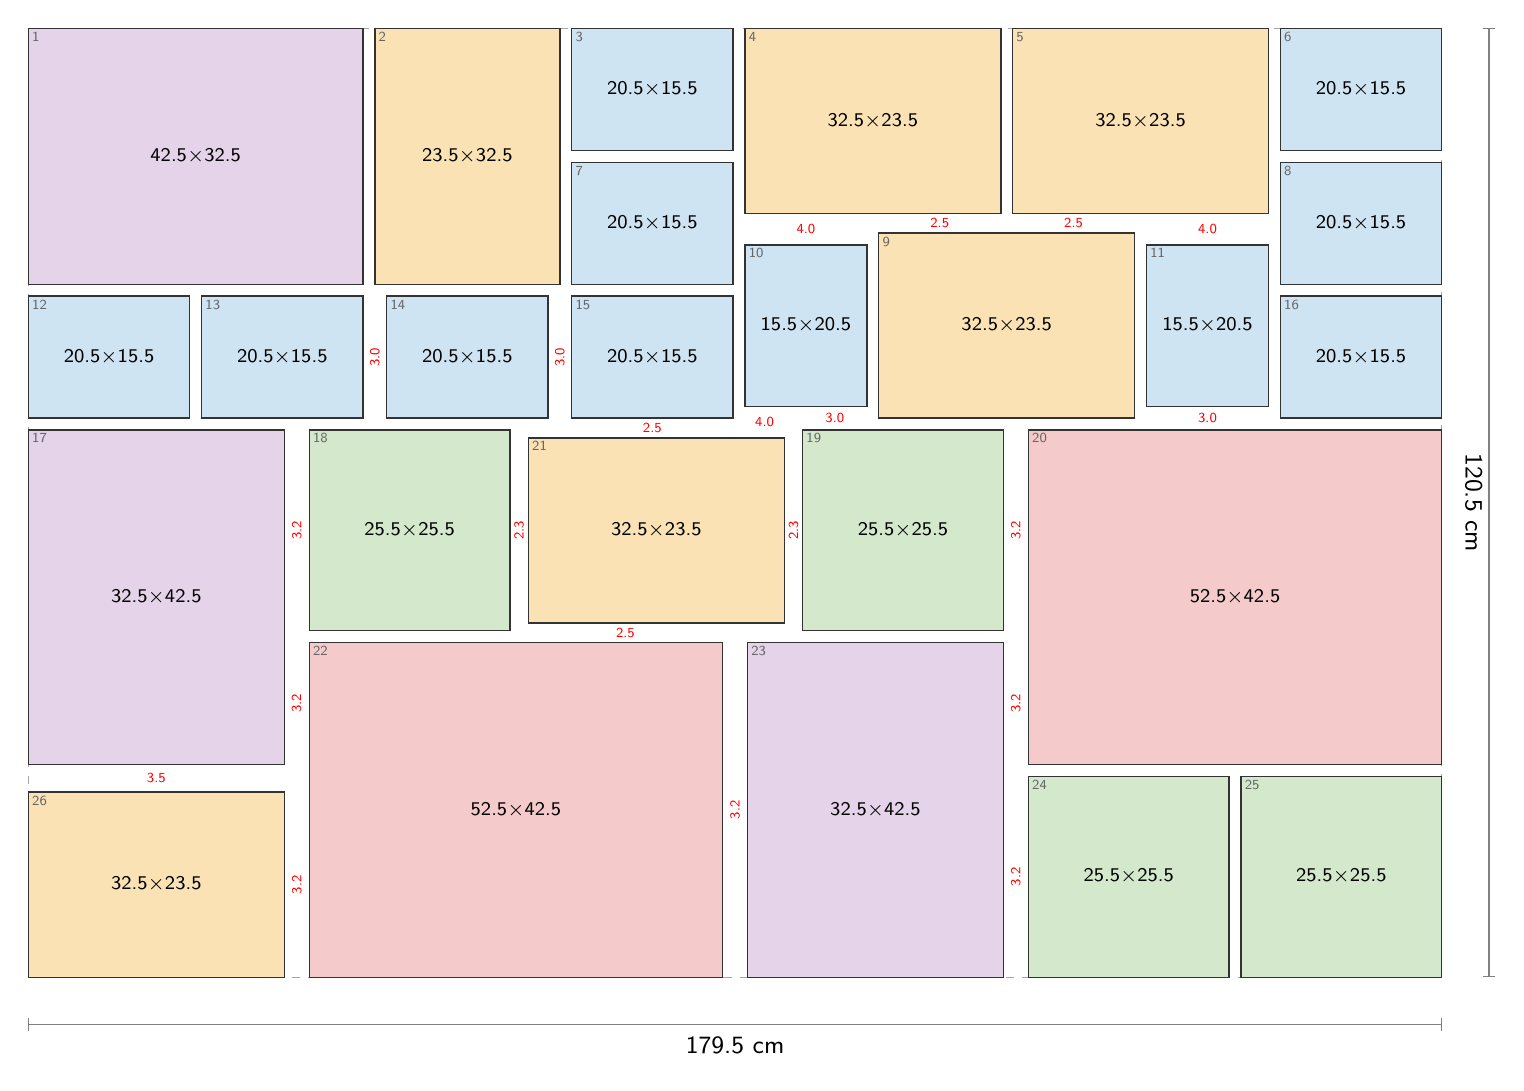
\begin{tikzpicture}[x=1mm, y=-1mm]
\draw[gray!70, dashed, line width=0.4pt] (0,0) rectangle (179.50,120.50);
\filldraw[fill=ft3, draw=black!80, line width=0.5pt] (0.00,0.00) rectangle (42.50,32.50);
\node[align=center, inner sep=0pt] at (21.25,16.25) {\scriptsize 42.5$\times$32.5};
\node[anchor=north west, inner sep=1.2pt, font=\tiny, text=black!60] at (0.00,0.00) {1};
\filldraw[fill=ft1, draw=black!80, line width=0.5pt] (44.00,0.00) rectangle (67.50,32.50);
\node[align=center, inner sep=0pt] at (55.75,16.25) {\scriptsize 23.5$\times$32.5};
\node[anchor=north west, inner sep=1.2pt, font=\tiny, text=black!60] at (44.00,0.00) {2};
\filldraw[fill=ft0, draw=black!80, line width=0.5pt] (69.00,0.00) rectangle (89.50,15.50);
\node[align=center, inner sep=0pt] at (79.25,7.75) {\scriptsize 20.5$\times$15.5};
\node[anchor=north west, inner sep=1.2pt, font=\tiny, text=black!60] at (69.00,0.00) {3};
\filldraw[fill=ft1, draw=black!80, line width=0.5pt] (91.00,0.00) rectangle (123.50,23.50);
\node[align=center, inner sep=0pt] at (107.25,11.75) {\scriptsize 32.5$\times$23.5};
\node[anchor=north west, inner sep=1.2pt, font=\tiny, text=black!60] at (91.00,0.00) {4};
\filldraw[fill=ft1, draw=black!80, line width=0.5pt] (125.00,0.00) rectangle (157.50,23.50);
\node[align=center, inner sep=0pt] at (141.25,11.75) {\scriptsize 32.5$\times$23.5};
\node[anchor=north west, inner sep=1.2pt, font=\tiny, text=black!60] at (125.00,0.00) {5};
\filldraw[fill=ft0, draw=black!80, line width=0.5pt] (159.00,0.00) rectangle (179.50,15.50);
\node[align=center, inner sep=0pt] at (169.25,7.75) {\scriptsize 20.5$\times$15.5};
\node[anchor=north west, inner sep=1.2pt, font=\tiny, text=black!60] at (159.00,0.00) {6};
\filldraw[fill=ft0, draw=black!80, line width=0.5pt] (69.00,17.00) rectangle (89.50,32.50);
\node[align=center, inner sep=0pt] at (79.25,24.75) {\scriptsize 20.5$\times$15.5};
\node[anchor=north west, inner sep=1.2pt, font=\tiny, text=black!60] at (69.00,17.00) {7};
\filldraw[fill=ft0, draw=black!80, line width=0.5pt] (159.00,17.00) rectangle (179.50,32.50);
\node[align=center, inner sep=0pt] at (169.25,24.75) {\scriptsize 20.5$\times$15.5};
\node[anchor=north west, inner sep=1.2pt, font=\tiny, text=black!60] at (159.00,17.00) {8};
\filldraw[fill=ft1, draw=black!80, line width=0.5pt] (108.00,26.00) rectangle (140.50,49.50);
\node[align=center, inner sep=0pt] at (124.25,37.75) {\scriptsize 32.5$\times$23.5};
\node[anchor=north west, inner sep=1.2pt, font=\tiny, text=black!60] at (108.00,26.00) {9};
\filldraw[fill=ft0, draw=black!80, line width=0.5pt] (91.00,27.50) rectangle (106.50,48.00);
\node[align=center, inner sep=0pt] at (98.75,37.75) {\scriptsize 15.5$\times$20.5};
\node[anchor=north west, inner sep=1.2pt, font=\tiny, text=black!60] at (91.00,27.50) {10};
\filldraw[fill=ft0, draw=black!80, line width=0.5pt] (142.00,27.50) rectangle (157.50,48.00);
\node[align=center, inner sep=0pt] at (149.75,37.75) {\scriptsize 15.5$\times$20.5};
\node[anchor=north west, inner sep=1.2pt, font=\tiny, text=black!60] at (142.00,27.50) {11};
\filldraw[fill=ft0, draw=black!80, line width=0.5pt] (0.00,34.00) rectangle (20.50,49.50);
\node[align=center, inner sep=0pt] at (10.25,41.75) {\scriptsize 20.5$\times$15.5};
\node[anchor=north west, inner sep=1.2pt, font=\tiny, text=black!60] at (0.00,34.00) {12};
\filldraw[fill=ft0, draw=black!80, line width=0.5pt] (22.00,34.00) rectangle (42.50,49.50);
\node[align=center, inner sep=0pt] at (32.25,41.75) {\scriptsize 20.5$\times$15.5};
\node[anchor=north west, inner sep=1.2pt, font=\tiny, text=black!60] at (22.00,34.00) {13};
\filldraw[fill=ft0, draw=black!80, line width=0.5pt] (45.50,34.00) rectangle (66.00,49.50);
\node[align=center, inner sep=0pt] at (55.75,41.75) {\scriptsize 20.5$\times$15.5};
\node[anchor=north west, inner sep=1.2pt, font=\tiny, text=black!60] at (45.50,34.00) {14};
\filldraw[fill=ft0, draw=black!80, line width=0.5pt] (69.00,34.00) rectangle (89.50,49.50);
\node[align=center, inner sep=0pt] at (79.25,41.75) {\scriptsize 20.5$\times$15.5};
\node[anchor=north west, inner sep=1.2pt, font=\tiny, text=black!60] at (69.00,34.00) {15};
\filldraw[fill=ft0, draw=black!80, line width=0.5pt] (159.00,34.00) rectangle (179.50,49.50);
\node[align=center, inner sep=0pt] at (169.25,41.75) {\scriptsize 20.5$\times$15.5};
\node[anchor=north west, inner sep=1.2pt, font=\tiny, text=black!60] at (159.00,34.00) {16};
\filldraw[fill=ft3, draw=black!80, line width=0.5pt] (0.00,51.00) rectangle (32.50,93.50);
\node[align=center, inner sep=0pt] at (16.25,72.25) {\scriptsize 32.5$\times$42.5};
\node[anchor=north west, inner sep=1.2pt, font=\tiny, text=black!60] at (0.00,51.00) {17};
\filldraw[fill=ft2, draw=black!80, line width=0.5pt] (35.67,51.00) rectangle (61.17,76.50);
\node[align=center, inner sep=0pt] at (48.42,63.75) {\scriptsize 25.5$\times$25.5};
\node[anchor=north west, inner sep=1.2pt, font=\tiny, text=black!60] at (35.67,51.00) {18};
\filldraw[fill=ft2, draw=black!80, line width=0.5pt] (98.33,51.00) rectangle (123.83,76.50);
\node[align=center, inner sep=0pt] at (111.08,63.75) {\scriptsize 25.5$\times$25.5};
\node[anchor=north west, inner sep=1.2pt, font=\tiny, text=black!60] at (98.33,51.00) {19};
\filldraw[fill=ft4, draw=black!80, line width=0.5pt] (127.00,51.00) rectangle (179.50,93.50);
\node[align=center, inner sep=0pt] at (153.25,72.25) {\scriptsize 52.5$\times$42.5};
\node[anchor=north west, inner sep=1.2pt, font=\tiny, text=black!60] at (127.00,51.00) {20};
\filldraw[fill=ft1, draw=black!80, line width=0.5pt] (63.50,52.00) rectangle (96.00,75.50);
\node[align=center, inner sep=0pt] at (79.75,63.75) {\scriptsize 32.5$\times$23.5};
\node[anchor=north west, inner sep=1.2pt, font=\tiny, text=black!60] at (63.50,52.00) {21};
\filldraw[fill=ft4, draw=black!80, line width=0.5pt] (35.67,78.00) rectangle (88.17,120.50);
\node[align=center, inner sep=0pt] at (61.92,99.25) {\scriptsize 52.5$\times$42.5};
\node[anchor=north west, inner sep=1.2pt, font=\tiny, text=black!60] at (35.67,78.00) {22};
\filldraw[fill=ft3, draw=black!80, line width=0.5pt] (91.33,78.00) rectangle (123.83,120.50);
\node[align=center, inner sep=0pt] at (107.58,99.25) {\scriptsize 32.5$\times$42.5};
\node[anchor=north west, inner sep=1.2pt, font=\tiny, text=black!60] at (91.33,78.00) {23};
\filldraw[fill=ft2, draw=black!80, line width=0.5pt] (127.00,95.00) rectangle (152.50,120.50);
\node[align=center, inner sep=0pt] at (139.75,107.75) {\scriptsize 25.5$\times$25.5};
\node[anchor=north west, inner sep=1.2pt, font=\tiny, text=black!60] at (127.00,95.00) {24};
\filldraw[fill=ft2, draw=black!80, line width=0.5pt] (154.00,95.00) rectangle (179.50,120.50);
\node[align=center, inner sep=0pt] at (166.75,107.75) {\scriptsize 25.5$\times$25.5};
\node[anchor=north west, inner sep=1.2pt, font=\tiny, text=black!60] at (154.00,95.00) {25};
\filldraw[fill=ft1, draw=black!80, line width=0.5pt] (0.00,97.00) rectangle (32.50,120.50);
\node[align=center, inner sep=0pt] at (16.25,108.75) {\scriptsize 32.5$\times$23.5};
\node[anchor=north west, inner sep=1.2pt, font=\tiny, text=black!60] at (0.00,97.00) {26};
\node[font=\tiny, text=red, fill=white, inner sep=0.3pt] at (115.75,24.75) {2.5};
\node[font=\tiny, text=red, fill=white, inner sep=0.3pt] at (98.75,25.50) {4.0};
\node[font=\tiny, text=red, fill=white, inner sep=0.3pt] at (132.75,24.75) {2.5};
\node[font=\tiny, text=red, fill=white, inner sep=0.3pt] at (149.75,25.50) {4.0};
\node[font=\tiny, text=red, fill=white, inner sep=0.3pt] at (102.42,49.50) {3.0};
\node[font=\tiny, text=red, fill=white, inner sep=0.3pt] at (93.50,50.00) {4.0};
\node[font=\tiny, text=red, fill=white, inner sep=0.3pt] at (149.75,49.50) {3.0};
\node[font=\tiny, text=red, fill=white, inner sep=0.3pt, rotate=90] at (44.00,41.75) {3.0};
\node[font=\tiny, text=red, fill=white, inner sep=0.3pt, rotate=90] at (67.50,41.75) {3.0};
\node[font=\tiny, text=red, fill=white, inner sep=0.3pt] at (79.25,50.75) {2.5};
\node[font=\tiny, text=red, fill=white, inner sep=0.3pt, rotate=90] at (34.08,63.75) {3.2};
\node[font=\tiny, text=red, fill=white, inner sep=0.3pt, rotate=90] at (34.08,85.75) {3.2};
\node[font=\tiny, text=red, fill=white, inner sep=0.3pt] at (16.25,95.25) {3.5};
\node[font=\tiny, text=red, fill=white, inner sep=0.3pt, rotate=90] at (62.33,63.75) {2.3};
\node[font=\tiny, text=red, fill=white, inner sep=0.3pt, rotate=90] at (125.42,63.75) {3.2};
\node[font=\tiny, text=red, fill=white, inner sep=0.3pt, rotate=90] at (97.17,63.75) {2.3};
\node[font=\tiny, text=red, fill=white, inner sep=0.3pt] at (75.83,76.75) {2.5};
\node[font=\tiny, text=red, fill=white, inner sep=0.3pt, rotate=90] at (89.75,99.25) {3.2};
\node[font=\tiny, text=red, fill=white, inner sep=0.3pt, rotate=90] at (125.42,85.75) {3.2};
\node[font=\tiny, text=red, fill=white, inner sep=0.3pt, rotate=90] at (125.42,107.75) {3.2};
\node[font=\tiny, text=red, fill=white, inner sep=0.3pt, rotate=90] at (34.08,108.75) {3.2};
\draw[Bar-Bar, gray] (0,126.50) -- (179.50,126.50) node[midway, below=1pt, font=\small, text=black] {179.5 cm};
\draw[Bar-Bar, gray] (185.50,0) -- (185.50,120.50) node[midway, right=1pt, font=\small, text=black, rotate=-90, anchor=north] {120.5 cm};
\end{tikzpicture}\\[4pt]
{\scriptsize Scale 1:10 (1 mm = 1 cm). Red numbers mark gaps that deviate from the nominal gap by more than 0.25 cm. Small grey numbers index the coordinate table.}
\end{minipage}\hfill
\begin{minipage}[t]{0.25\textwidth}\vspace{0pt}
\small
\begin{tabular}{@{}l l@{}}
\toprule
Outer size & 179.5 $\times$ 120.5 cm \\
Nominal gap & 1.5 cm \\
Actual gaps & 1.5 -- 4.0 cm \\
Max.\ deviation & 2.5 cm \\
Mean deviation & 0.60 cm \\
Border notches & bottom 10 cm, left 4 cm \\
Corners filled & 4 / 4 \\
Frames used & 26 of 28 \\
Large frames & {\scriptsize 2, not touching, min.\ dist.\ 95 cm} \\
Entropy & 0.77 \\
\quad {\scriptsize mix / variety} & {\scriptsize 0.83 / 0.78} \\
\quad {\scriptsize stagger / lines} & {\scriptsize 0.49 / 1.00 (1 through)} \\
\bottomrule
\end{tabular}

\vspace{8pt}
\scriptsize
\begin{tabular}{@{}c l l r r@{}}
\toprule
 & outer w $\times$ h (cm) &  & used & have \\
\midrule
\tikz[baseline=-0.6ex]\fill[ft0,draw=black!60] (0,0) rectangle (1.2ex,1.2ex); & 20.5$\times$15.5 & L & 9 & 9 \\
\tikz[baseline=-0.6ex]\fill[ft0,draw=black!60] (0,0) rectangle (1.2ex,1.2ex); & 15.5$\times$20.5 & P & 2 & 2 \\
\tikz[baseline=-0.6ex]\fill[ft3,draw=black!60] (0,0) rectangle (1.2ex,1.2ex); & 32.5$\times$42.5 & P & 2 & 2 \\
\tikz[baseline=-0.6ex]\fill[ft3,draw=black!60] (0,0) rectangle (1.2ex,1.2ex); & 42.5$\times$32.5 & L & 1 & 1 \\
\tikz[baseline=-0.6ex]\fill[ft1,draw=black!60] (0,0) rectangle (1.2ex,1.2ex); & 32.5$\times$23.5 & L & 5 & 5 \\
\tikz[baseline=-0.6ex]\fill[ft1,draw=black!60] (0,0) rectangle (1.2ex,1.2ex); & 23.5$\times$32.5 & P & 1 & 1 \\
\tikz[baseline=-0.6ex]\fill[ft2,draw=black!60] (0,0) rectangle (1.2ex,1.2ex); & 25.5$\times$25.5 &  & 4 & 5 \\
\tikz[baseline=-0.6ex]\fill[ft4,draw=black!60] (0,0) rectangle (1.2ex,1.2ex); & 42.5$\times$52.5 & P & 0 & 1 \\
\tikz[baseline=-0.6ex]\fill[ft4,draw=black!60] (0,0) rectangle (1.2ex,1.2ex); & 52.5$\times$42.5 & L & 2 & 2 \\
\bottomrule
\end{tabular}

\vspace{8pt}
{\bfseries Positions} (top-left corner, cm)\\[2pt]
\tiny
\begin{tabular}{@{}r l r r@{}}
\toprule
\# & frame w $\times$ h & x & y \\
\midrule
1 & 42.5 $\times$ 32.5 & 0.0 & 0.0 \\
2 & 23.5 $\times$ 32.5 & 44.0 & 0.0 \\
3 & 20.5 $\times$ 15.5 & 69.0 & 0.0 \\
4 & 32.5 $\times$ 23.5 & 91.0 & 0.0 \\
5 & 32.5 $\times$ 23.5 & 125.0 & 0.0 \\
6 & 20.5 $\times$ 15.5 & 159.0 & 0.0 \\
7 & 20.5 $\times$ 15.5 & 69.0 & 17.0 \\
8 & 20.5 $\times$ 15.5 & 159.0 & 17.0 \\
9 & 32.5 $\times$ 23.5 & 108.0 & 26.0 \\
10 & 15.5 $\times$ 20.5 & 91.0 & 27.5 \\
11 & 15.5 $\times$ 20.5 & 142.0 & 27.5 \\
12 & 20.5 $\times$ 15.5 & 0.0 & 34.0 \\
13 & 20.5 $\times$ 15.5 & 22.0 & 34.0 \\
14 & 20.5 $\times$ 15.5 & 45.5 & 34.0 \\
15 & 20.5 $\times$ 15.5 & 69.0 & 34.0 \\
16 & 20.5 $\times$ 15.5 & 159.0 & 34.0 \\
17 & 32.5 $\times$ 42.5 & 0.0 & 51.0 \\
18 & 25.5 $\times$ 25.5 & 35.7 & 51.0 \\
19 & 25.5 $\times$ 25.5 & 98.3 & 51.0 \\
20 & 52.5 $\times$ 42.5 & 127.0 & 51.0 \\
21 & 32.5 $\times$ 23.5 & 63.5 & 52.0 \\
22 & 52.5 $\times$ 42.5 & 35.7 & 78.0 \\
23 & 32.5 $\times$ 42.5 & 91.3 & 78.0 \\
24 & 25.5 $\times$ 25.5 & 127.0 & 95.0 \\
25 & 25.5 $\times$ 25.5 & 154.0 & 95.0 \\
26 & 32.5 $\times$ 23.5 & 0.0 & 97.0 \\
\bottomrule
\end{tabular}
\end{minipage}
\clearpage

\end{document}
